\documentclass[a4paper, 12pt]{article}
\usepackage{subfiles}
\usepackage{Main/nea}
%Title and headings
\title{\textbf{Computer Science NEA: Momentum}}
\author{Ojas Tiwari 13R}
\date{}
\begin{document}

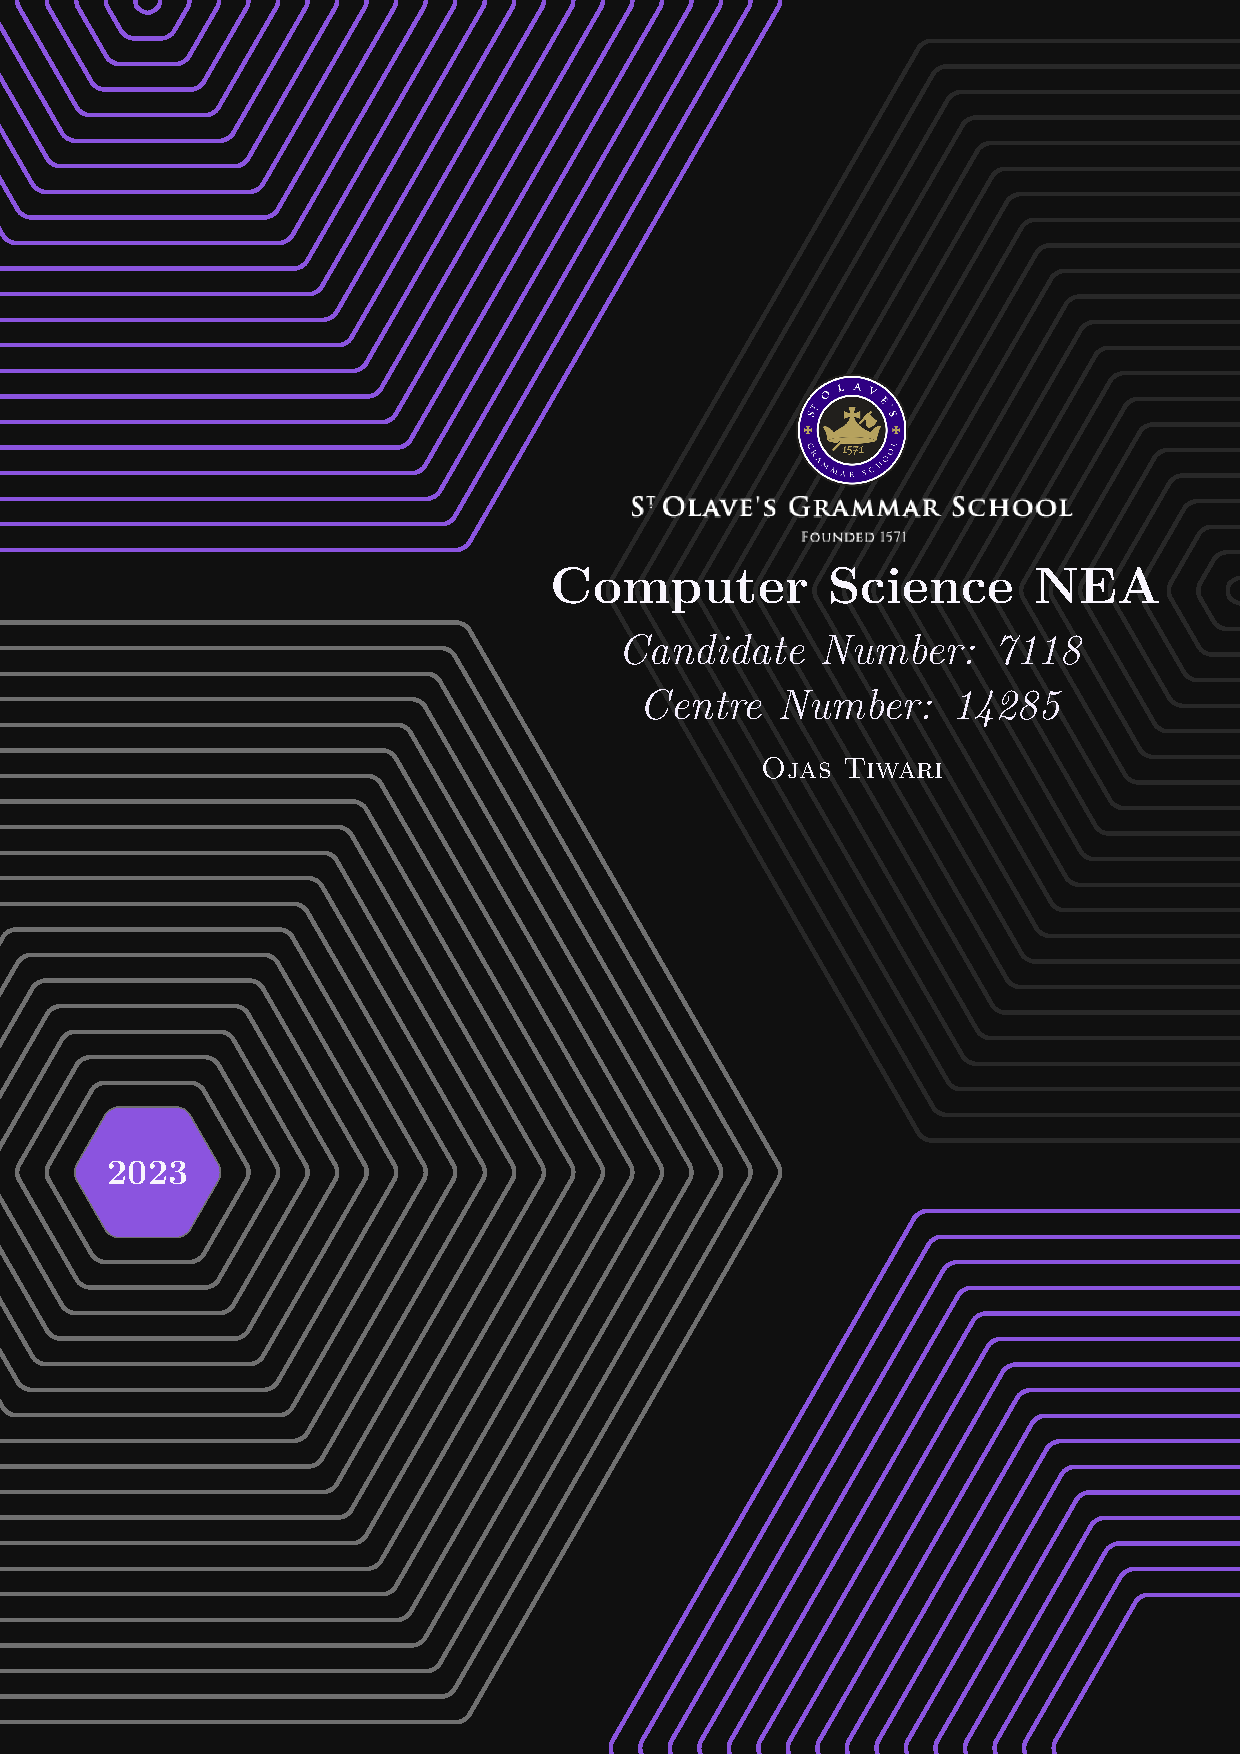
\includepdf[pages=1]{Main/Front_Cover.pdf}

\sffamily
\maketitle
\thispagestyle{plain}

{\large Throughout this document, I have used red text to denote links, primarily to YouTube videos demonstrating different sections of my project. Many of the figures in the development section are clickable and will lead to videos. These videos are highly relevant to the project, and prove that it does indeed work, since many aspects of my project are graphical, and so a video is the best way to illustrate them in action.}

\clearpage

\tableofcontents
\clearpage

%Put subsections in in seperate files 
\section{Analysis}
\subsection{Problem Definition}

For my project, I will be creating a game, playable on a computer, that will allow people with limited time to still be able to enjoy playing a fun and engaging game. To begin with, I will list the current problems with games that are still playable.

\begin{enumerate}[label=\textbf{\arabic*.}]
    \item \textbf{Games have very long rounds} - This causes people to be involved in the same game for a much longer period of time, and results in there being time to only play one or two rounds at most, and potentially having to leave mid-way through a round if another tasks needs to be taken care of. This can result in frustration, especially if the person had favourable conditions, and may lead to them leaving the game entirely. 
    \item \textbf{Queue times for games are becoming very long} - This usually accompanies games which have long round times as the people who are playing are most likely in a game already, and so therefore, there are very few people left that can form a lobby. This also occurs whenever there is strict matchmaking rules, such as based on MMR, or region. This causes there to be a smaller pool of players that can be in the same lobby, and therefore, it is much more difficult to create a lobby in a short period of time.
    \item \textbf{Overly complicated} - Modern games are starting to have lots of additional features, due to the large amount of computing power that is available, and whilst this does mean that there are lots of things to experiment with in the game, it can make it overwhelming at times, and very competitive. This will suit some people, but for casual players, having a game with lots of different details can be very difficult to learn, and so discourages them from playing.
    \item \textbf{Cosmetic items} - Whilst these do add aesthetic appeal to the game, in most games they are locked behind a paywall, whilst leaving players who do not wish to spend money on a game feeling left out.
    \item \textbf{Intensive Hardware Requirements} - As the average PC has become more powerful, older devices can no longer keep up with modern games, and this means that lots of people are simply unable to play with people who have a modern PC. This is mostly due to the large maps and intensive graphics, that require lots of CPU and GPU processing power. Most games do have options to reduce the graphics quality, but they still require newer hardware to be able to play. Someone who is not in a position to purchase a newer device will then be excluded from playing.
    \item \textbf{Too strategy based} - An issue within the shooter genre which I aim to fix is that games are becoming very strategy based instead of focusing on fast-paced intense gameplay. This is done by reducing the player's movement speed and by making maps very intricately designed. However, this can make it boring at times, because players spend a lot of time hiding in spots, or setting up traps instead of fighting with other players. This also leads to the sensation that the game is boring, leading people to not want to play anymore.
    \item \textbf{Too competitive} - Many games have a match-making rating (MMR for short), which changes depending on whether you won or lost the game. This causes people to feel pressured during the game, and this can cause them to not enjoy playing, especially if they are casual players.
    \item \textbf{Lack of competent bots} - Many bots in games lack any proficiency in the game, and this means that they are not able to be put in a game if there are not enough players, or if someone leaves the game. This also means that if someone wants to train certain mechanics in the game, they do not have any quick way of checking. "Training" modes in most games are very empty, and usually consist of empty maps, or stationary targets that cannot retaliate.
\end{enumerate}

Based on this, I wanted to see how these factors impacted people's enjoyment of shooter games, and what my project should focus on in order to make the game more accessible and enjoyable to a wider range of people.

\subsection{Analysis of Existing Solutions}

Next, I will look at some other games that are available currently, and what their positive and negative aspects are, as well as what things I can learn from them and implement into my project.


\vs

\subsubsection{Chess}

Chess is a classic board game that is enjoyed by many people globally and has been around for centuries, and has been on the internet since the early 2000s. It involves moving pieces on a board according to a set of rules, and the player who loses is the one who no longer has any legal moves remaining. Recently, chess websites have seen a boom in popularity. Despite this, there are many people who don't enjoy or understand chess, and many that do. \cite{chess}
\begin{figure}[h!t]

\begin{annotatedFigure}
	{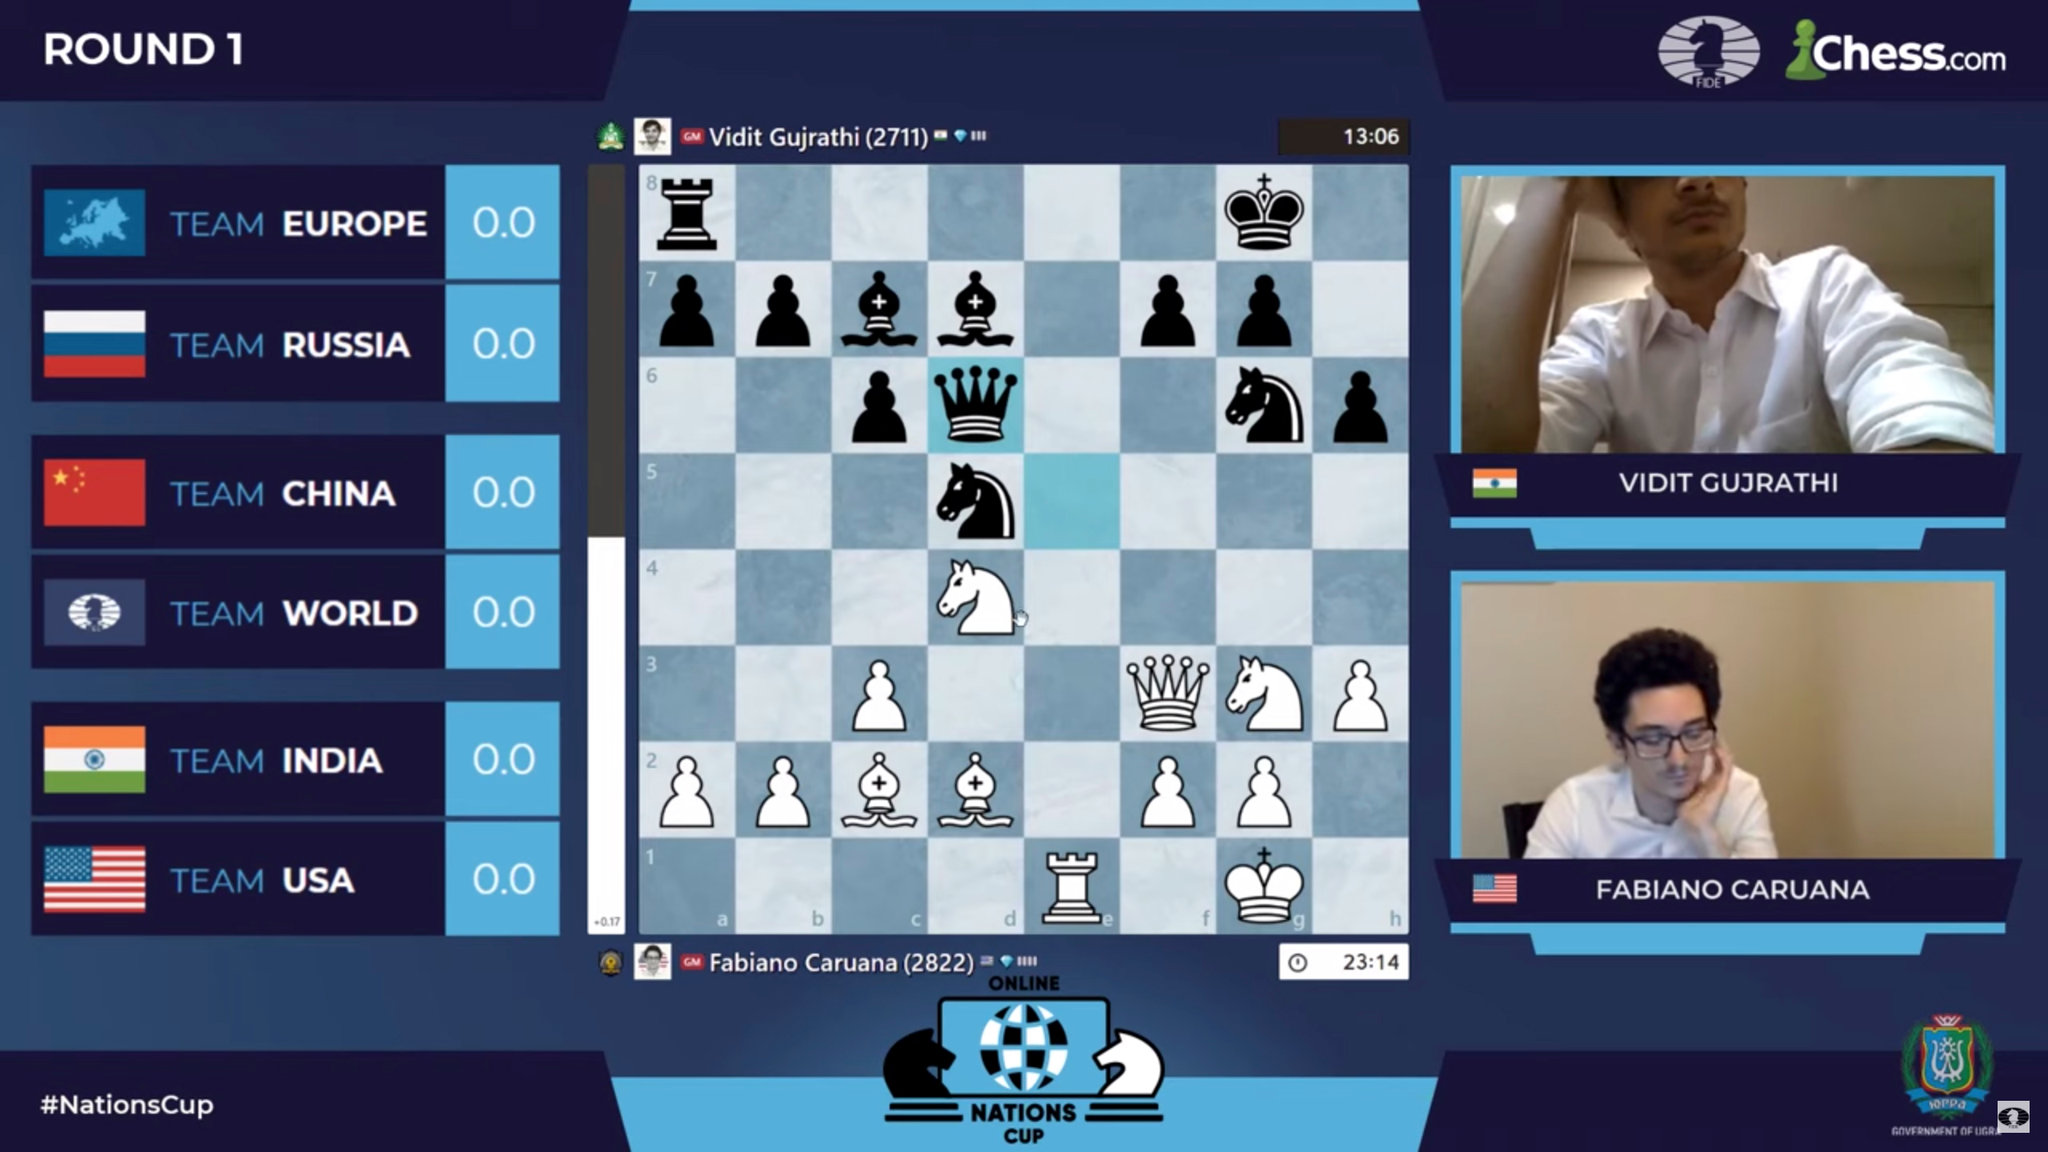
\includegraphics[width=1.0\linewidth]{Analysis/Images/ChessScreenshot.jpg}}
	\annotatedFigureBox{0.617,0.854}{0.696,0.9092}{A}{0.617,0.854}%bl
	\annotatedFigureBox{0.28,0.1773}{0.313,0.8736}{B}{0.28,0.1773}%bl
	\annotatedFigureBox{0.303,0.8416}{0.493,0.9305}{C}{0.303,0.8416}%bl
	\annotatedFigureBox{0.5,0.18}{0.693,0.2253}{D}{0.5,0.18}%bl
\end{annotatedFigure}
\caption{\textbf{Chess} - An image of a live stream of a professional chess tournament from }
\label{fig:chess_tournament}
\end{figure}

\textcolor{cyan}{\textbf{Analysis:}}
In box A, we can see the time left for each player in the game. This is important, since chess is usually played with a clock, and so it is useful to have this visible clearly to both players, but not in such a way that is intrusive on the player's vision of the board. Placing this near the corner of the board means that a player can easily how much time they or the opponent has left, but not be distracted by the clock.

\vs
In box B, we can see the computer analysis of the game. Normally, this would not be present during a rated game, but during live streams or analysis of games, it is put there to provide more information to players. Generally, chess positions are very complex, and therefore, it may not be obvious to inexperienced players what is going on, and so this is quite a useful tool. For players who are learning the game, it can be helpful to see where they may have blundered, and what moves would be better in that position.

\vs
In box C, we display the name and the rating of the player. This tells you who you are playing against and what their ELO is, which is a ranking often used in chess. This isn't particularly relevant, but it shows you that you are playing against a real player, which is a concern for some people. Additionally, if you want to play against friends, it's useful to make sure that you are playing against the right person. Another advantage is that it shows you if you are matched with a novice player or someone who has played the game for a long time, which may not affect the actions of the player directly, but it will inform them as to the level of play they can expect in the game.

\vs
Finally, the lettering on the bottom in Box D and the left edge of the board lets us easily identify which square a certain piece is on, and this is helpful when communicating with other players about moves, and is the standard notation for chess globally. This is useful, for example, for a coach who might want to help their play spot a move on the board.
\vs


\textcolor{green}{\textbf{Positives:}}
Chess is another game that satisfies my criteria and has another benefit. Online chess also lets people choose what length of game they want to play, ranging anywhere from 15 seconds to an hour. This is useful as it allows people to dedicate as much time as they want and no more than that for certain. It also has a ranking system, and is relatively easy to pick up. It is a reliable platform, and has been used for professional tournaments, such as during the pandemic, as seen in Figure \ref{fig:chess_tournament}. 
\vs


\textcolor{red}{\textbf{Negatives:}} Again, it's not an shooter game and not everyone likes or enjoys playing it. It isn't as visually stimulating as other games and for some people that is a major issue. In recent times, throughout the pandemic, chess gained a lot of popularity and many streamers became very popular and chess websites like \emph{chess.com} were not able to keep up with the demand, reaching 2 million players per day at one point. Another issue is that there is a very steep learning curve, and so the game can feel unrewarding when initially starting out, and requires a very large time investment to get good at the game. This is not always a possibility, and so people may feel unmotivated to play as it takes so long to understand how to becomes better at the game.
\vs


\textcolor{violet}{\textbf{Ideas taken:}} There are different time controls, which can be desirable so people can play as many rounds as they want depending on how much time they have, which would be ideal in my project, as time is a major restriction for most people. Additionally, the website \emph{chess.com} has bots on it that you can play against to practice with.
\vs


\subsubsection{Unreal Tournament}

Unreal Tournament is a series of games made by Epic Games starting in 1999 and the final game due to be released in 2017, but being cancelled before it was ever released. This final iteration was released in pre-alpha, but of course was not a final product. There is still some footage from the pre-alpha, so we will analyse that here.
\vs
\begin{figure}[h!t]
\begin{annotatedFigure}
	{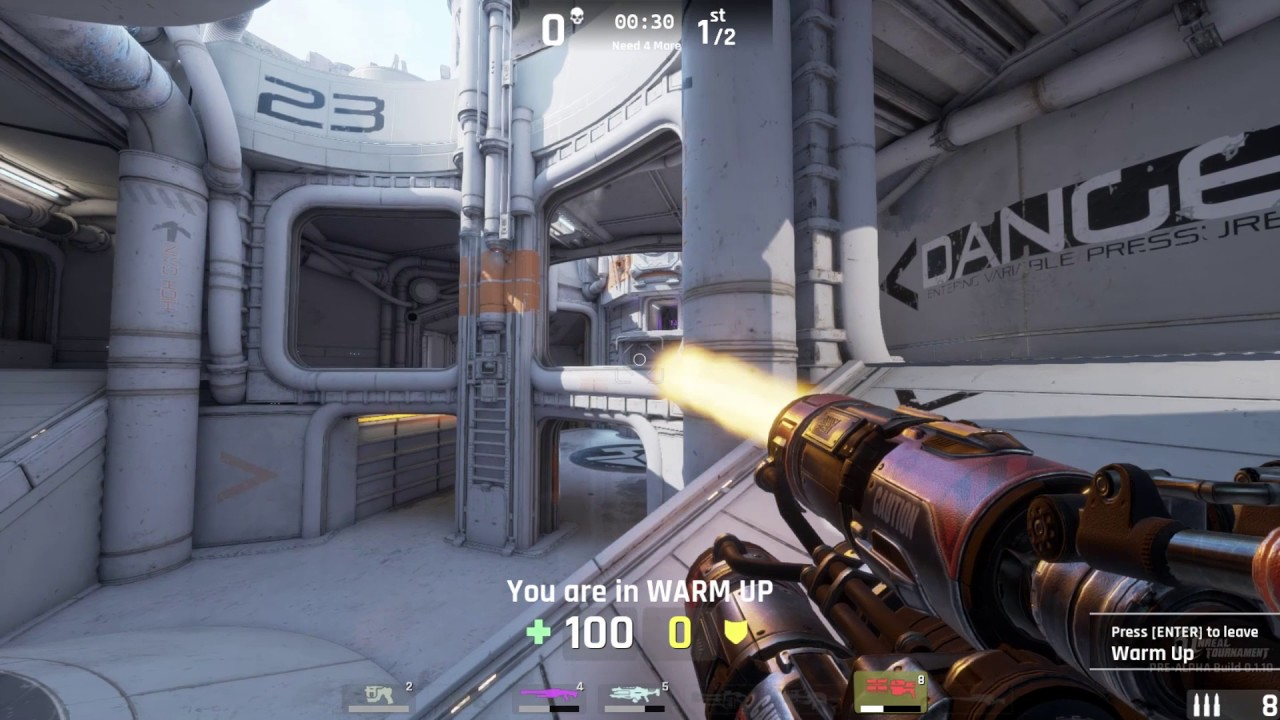
\includegraphics[width=1.0\linewidth]{Analysis/Images/UnrealTournament.jpg}}
	\annotatedFigureBox{0.4052,0.9022}{0.5982,0.9984}{E}{0.4052,0.9022}%bl
	\annotatedFigureBox{0.393,0.0891}{0.5972,0.1703}{F}{0.393,0.1703}%tl
	\annotatedFigureBox{0.842,0.0603}{0.9982,0.1593}{G}{0.842,0.0603}%bl
	\annotatedFigureBox{0.2580,0.000}{0.7380,0.0831}{H}{0.2580,0.0831}%tl
\end{annotatedFigure}
\caption{\textbf{Unreal Tournament} - Screenshot taken during gameplay from \cite{ut}}
\label{fig:ut}
\end{figure}

\textcolor{cyan}{\textbf{Analysis:}}
Starting in Box E, we can see that we gain important information about the game here in a concise way. We find what we need to do to win the game, how long is left in the game, and what position we are in the game. This is important for a player to know as it may advise them on how to proceed. For example, if there is a large amount to be done in order to win the game, the player knows to play more aggressively. This justifies it being there, because it informs the player's decisions during the game.

\vs
In box F, we see the player's health and shield levels. This is important information, since if the player is low health, they may choose to heal instead of engaging in combat, and vice versa. The information presented on the screen is in a large font which makes it easy to see the information at a glance, but not so big as to distract from the main information on the screen (ie. the game itself).

\vs
In Box H, we can see the player's weapons as well as how much ammo each one has. This allows a player to see what they have currently selected, and we can also see that on the screen. This is justified because having this information present allows a player to make an informed decision on what they should do next. For example, if they are on low ammo on all of their weapons, they should reload, or look for more ammo. It also tells them what types of strategies may work in the game, since different weapons have different characteristics which are more favourable in certain scenarios. For example, a sniper rifle might be more useful in a long-range encounter, but a shotgun might work better in close quarters. Having this information is useful to a player, and without it, they would struggle, and so it's justified to be there. It's isn't the most important piece of information however, so it doesn't occupy too much of the screen, and is at the bottom.

\vs
Finally, in Box G, we see the option to leave the warm up and to join the actual game. This is useful because it gives the player control over what they want to do, and it tells them what mode they are in currently. This is justified because new players may be confused about what they are doing if they haven't played before, or have been told what each mode is. Therefore, having a label describing what they are currently doing is incredibly helpful to them.
\vs


\textcolor{green}{\textbf{Positives:}} \emph{Unreal Tournament} is also a shooter game. The shortest game length is 4 minutes according to Wikipedia whereas I hope to make that 6 minutes, but in 3 separate rounds. The advantage of this is to make it so that people are able to dedicate less time to a specific round, so even if they lose, they still have a share of the time to win the round. 
\vs


\textcolor{red}{\textbf{Negatives:}} It is primarily a single-player game, which many people can find boring, and not as interactive as a multi-player game.An issue with Unreal Tournament is that and no servers are currently running, and so it results in people not being able to play it at all. This means that there are very few games similar to Unreal Tournament that are still available.
\vs


\textcolor{violet}{\textbf{Ideas taken:}} There are lots of different mechanics within the game such as those seen in \href{https://www.youtube.com/watch?v=knSzJbkofek}{this video}. These are inspirations for what can be implemented in my game, and what other things can be included in order to make it more dynamic.
\vs


\subsubsection{Valorant}

\emph{Valorant} is a highly successful First Person Shooter Game made by Riot Games.

\begin{figure}[h!t]

\begin{annotatedFigure}
	{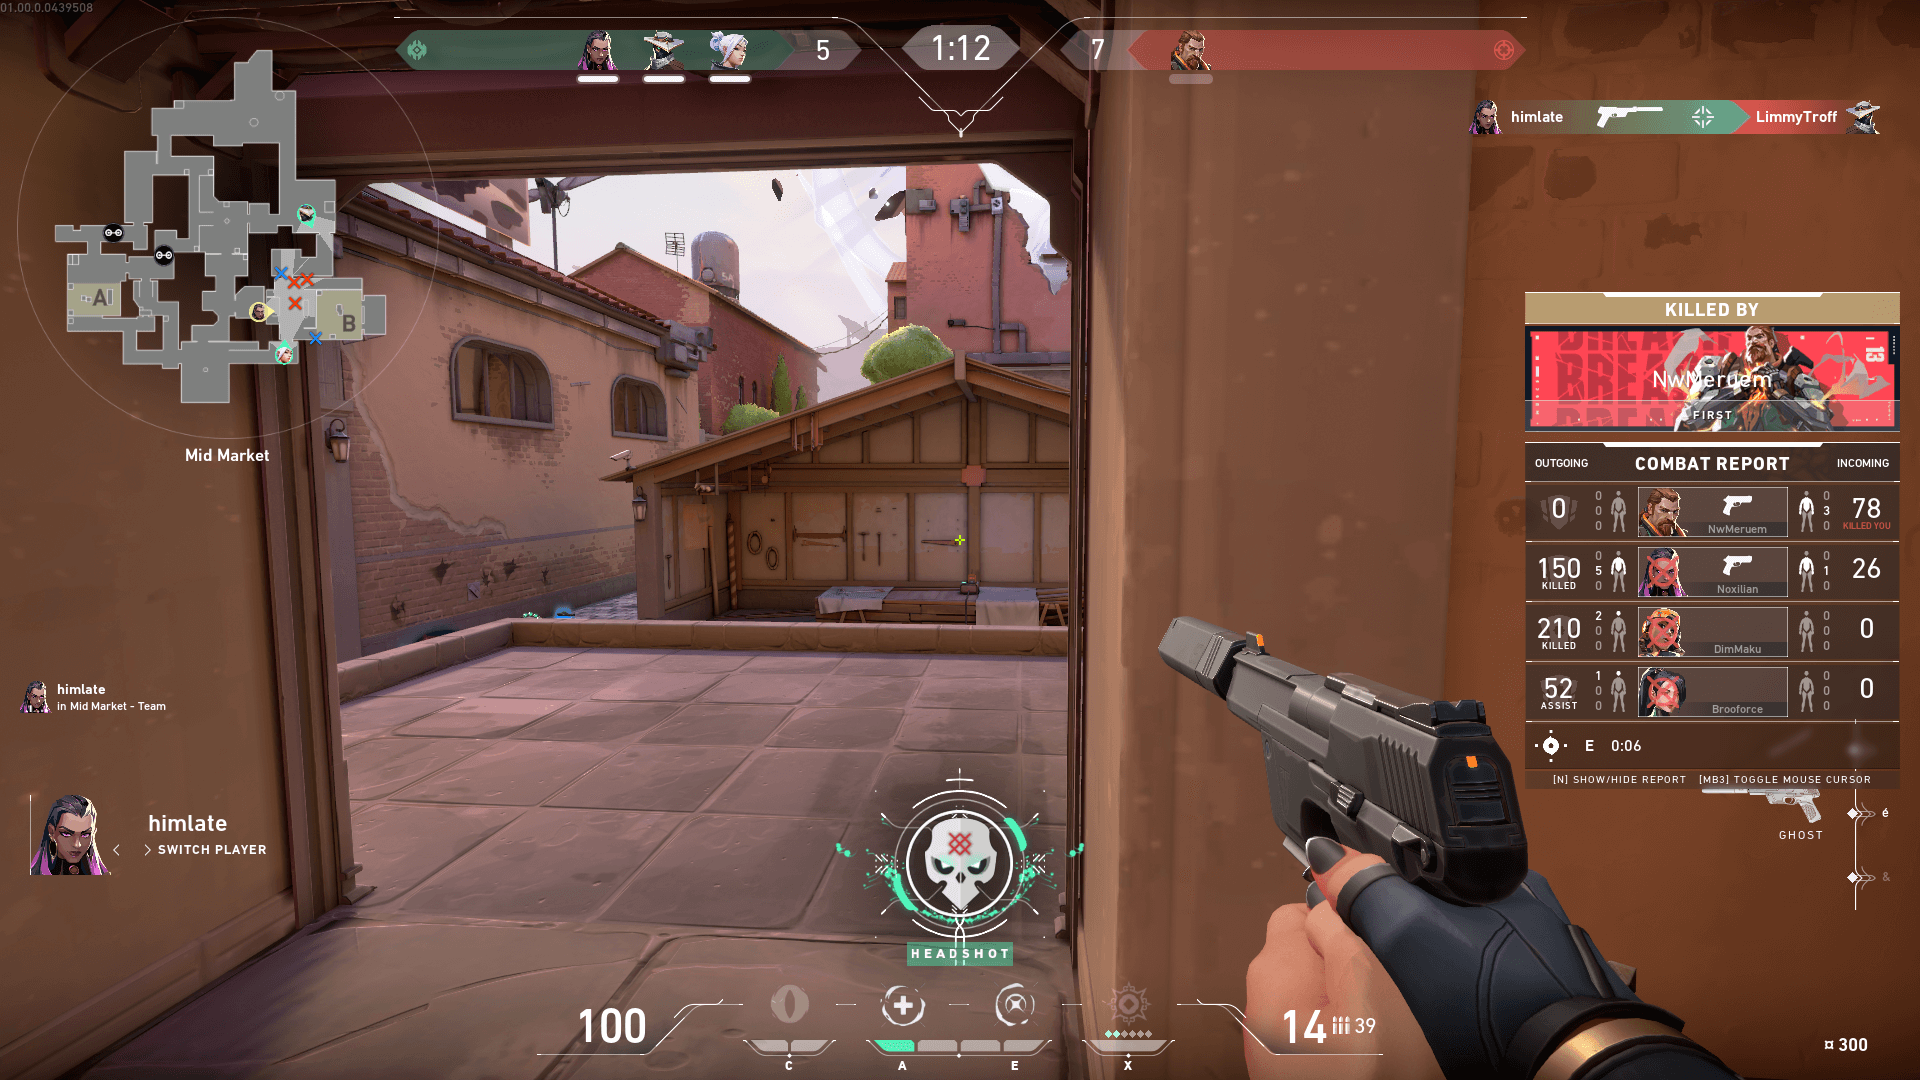
\includegraphics[width=1.0\linewidth]{Analysis/Images/ValorantScreenshot.png}}
	\annotatedFigureBox{0.189,0.9106}{0.8052,0.9949}{I}{0.189,0.9106}%bl
	\annotatedFigureBox{0.0252,0.6109}{0.2132,0.9639}{J}{0.0252,0.6109}%bl
	\annotatedFigureBox{0.757,0.848}{0.9862,0.938}{K}{0.757,0.848}%bl
	\annotatedFigureBox{0.215,0}{0.7762,0.1009}{L}{0.215,0.1009}%tl
\end{annotatedFigure}

\caption{\textbf{Valorant} - Screenshot of gameplay from \cite{val}}
\label{fig:valorant}

\end{figure}

\vs
%Screenshot Credit: https://interfaceingame.com/screenshots/valorant-headshot/

\textcolor{cyan}{\textbf{Analysis:}}
In box I, we see the players remaining in each team, the time left in the round, and the score. This is helpful because it informs all players of how they should play, and what strategies are most likely to get them a win in each round. For example, if one team has more players than another at some point in a round (due to some players being eliminated), they know that they can quite easily get a win.

\vs
In box J, we see a mini-map. This is quite a common feature amongst shooter games, and it allows players to see where they are, where their team-mates are, and where objectives are. This allows players to see the quickest way to get to their desired position. For new players, who may not know the layout and structure of the maps, it provides an intuitive way of understanding where they are relative to other players, as well as which direction they are facing. This is not made too large as too distract the player, but not too small so that the player cannot accurately see what is happening. Furthermore, the map is placed in the top left corner, because this allows the player to have a clear view of the middle row of their screen, which is where most of the action happens.

\vs
In box K, we see the elimination feed. This tells everyone in the game who has just been eliminated that round, which tells teams important information that informs their decisions. For similar reasons to the ones mentioned above, it is also placed in a corner, as it isn't the most important information the player is receiving.

\vs
At the bottom of the screen, we have box L. It shows the player the health that they have on the left hand side, the abilities in the middle, and the ammo left on the right hand side. The weapons that they have is on the right hand side of the screen, but was obscured in the image due to a popup from the game. The screen shown is from the view of a player who was eliminated earlier that round and is currently spectating one of their teammates. This is a useful feature because it means that a player is not just waiting around between rounds if they are eliminated, and can still be involved in the thrill of the game. From the viewpoint of a player who is still playing the middle of the right hand side of the screen would show the selection of weapons available to the player to use, and which button to press to select it. Icons are used to represent each weapon, because they each have distinctive shapes which are easy to identify. This is essential, because First Person Shooters are quite fast-paced with split-second decisions needing to be made, and so therefore, having a quickly recognisable symbol is crucial.


\vs
\textcolor{green}{\textbf{Positives:}} \emph{Valorant} is also a very successful game that is a shooter game. It also uses vibrant colours and interesting map design, combined with a wide range of abilities depending on the character taken. This allows for a lot of different situations to arise and means that the games are always varied and exciting. The UI is slightly larger than it is for other games, but it is still kept minimal and only conveys essential information. There is also a voice chat feature which allows players on the same team to talk to each other in real time during the game.

\vs
\textcolor{red}{\textbf{Negatives:}} The rounds are extremely long, even lasting over 45 minutes. This is a major problem for people who are on limited time, as they are much less likely to start a new game as they don't want to have to leave mid-way. This leads to people abandoning the game altogether, and subsequently not being able to play even if they do have a little bit of time.

\vs
\textcolor{violet}{\textbf{Ideas Taken:}} It has a very high skill ceiling (the maximum skill that a player can reach in the game) due to a large number of mechanics and different characters, which all specialise in different skills. This keeps the game interesting and unique. This is something that I am to replicate in my project by using movement mechanics, which allow a player to move very fast in a short period of time, and potentially "out-play" opponents. This adds to the intensity of the game, and also means that despite the short rounds people will see a lot of action in the games.
\vs

\subsubsection{Rocket League}

\emph{Rocket League} is a game made by Psyonix, and is played by millions. It involves scoring goals, using cars which can be driven around the map and even on the walls. The cars have boost which allows them to drive at extremely high speeds, but needs to be recharged as there is only a limited amount of it. This can be done by driving over pads or cylinders on the field which refills the boost by different amounts. The game has a very simple premise, but there are many mechanics within the game, which can be chained together to make complex motions, keeping the game interesting.


\begin{figure}[h!t]

\begin{annotatedFigure}
	{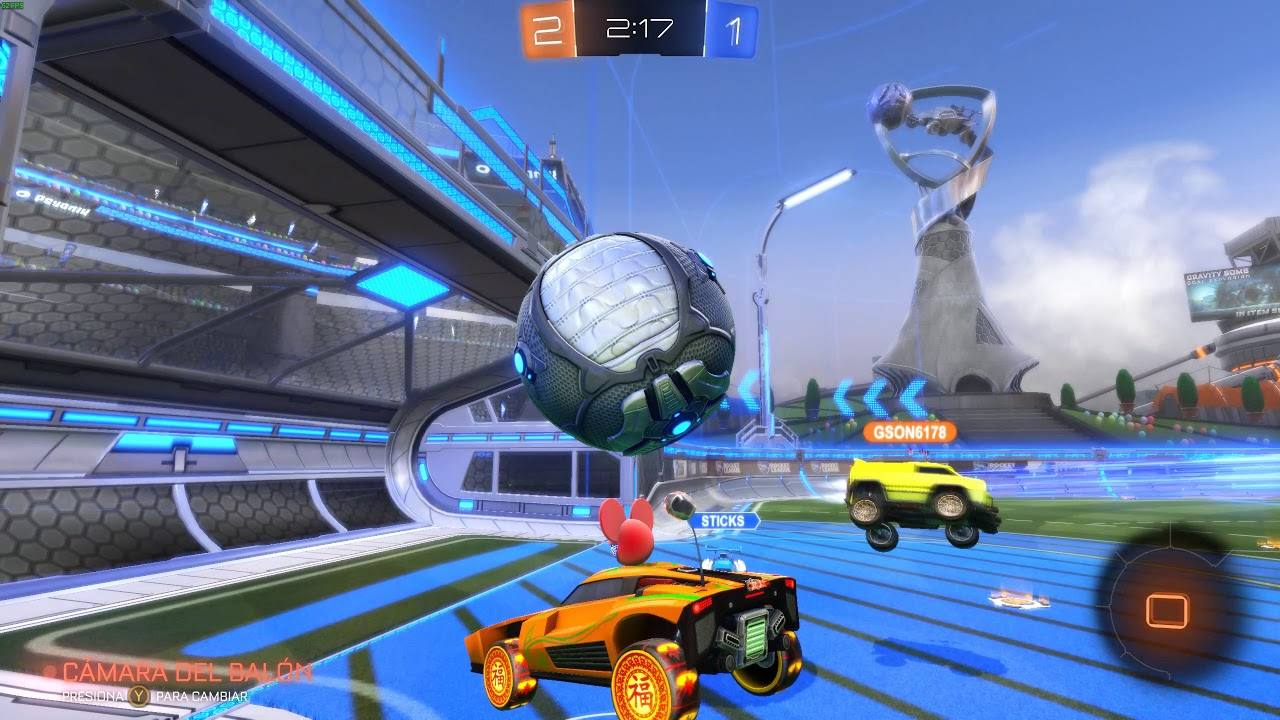
\includegraphics[width=1.0\linewidth]{Analysis/Images/RocketLeague.jpg}}
	\annotatedFigureBox{0.399,0.9081}{0.6,0.9999}{M}{0.399,0.9081}%bl
	\annotatedFigureBox{0.664,0.3693}{0.7583,0.4351}{N}{0.664,0.3693}%bl
	\annotatedFigureBox{0.8463,0.035}{0.9825,0.2769}{O}{0.8463,0.2769}%tl
	\annotatedFigureBox{0.017,0}{0.267,0.1045}{P}{0.267,0.1045}%tr
\end{annotatedFigure}
\caption{\textbf{Rocket League} - Screenshot of some gameplay}
\label{fig:rl}

\end{figure}

\textcolor{cyan}{\textbf{Analysis:}} Firstly, we can see on the screen that there is a lot of vibrant colours which helps to exchange players and gives it an exciting feel. In Box M, we can see a lot of information, including the time left in the game and the number of goals that each team has. The score is colour-coded depending on the colour of the team. This is very helpful since the colour of the player's car matches which team they are on, and so it is easy to spot how many goals a player's team has.

\vs
Additionally, in Box N, we can the player tags. The game is very fast-paced and therefore, it can sometimes be difficult to see what is going on in the game. The players have large labels with their team colour and their username on it which makes it much easier to spot players, especially when they are further away and not close to each other.

\vs
In box O, we can see the amount of boost that the player has. This is a number between 0 and 100 and will allow the player to 


\textcolor{green}{\textbf{Positives:}} Rocket League is extremely vibrant, with lots of customisation options for your car. This provides a lot of flexibility and adds character to the game. Additionally, there is a lot of mechanics that can be used and discovered, which keeps the game fresh. This allows for a lot of engagement with the players and means that they are never bored as there is always something to learn or do within Rocket League.

\vs

\textcolor{red}{\textbf{Negatives:}} It's not an FPS game, and is incredibly frustrating to learn initially, and requires several hundred hours of gameplay in order to become an "average" player. This results in many people finding themselves unable to commit the time needed to become better at the game or progress at all. Additionally, the game is incredibly competitive due to the competitive game mode, and this can be too intense for some people. For example, it is possible to have a very involved game, but not be intense.
\vs

\textcolor{violet}{\textbf{Ideas taken:}} Vibrant colours are often quite appealing and makes it much easier to understand what is going on in the game. The small map sizes and relatively low render requirements make it much more easily accessible to people on low-end setups, and means that a much more powerful computer is able to run the game at a much better quality. Having simple game mechanics is often enough to keep people engaged, provided that they are unique, such as the ability to reset jumps from the ceiling, and even the ball, that is possible in Rocket League. This allows players to continually learn and improve. However, it is key that these do not make the game unplayable for anyone who doesn't know the mechanic. The UI is very minimal, and shows only what the player really needs to see, such as the boost, the score, and the time. This helps to make the game not feel overwhelming.


\subsubsection{The Elo Algorithm}
\vs
Most games require a lot of time in order to "get good" at a game, or to acquire some proficiency in it, which can be demoralising and means people stop playing. Matchmaking that links players of all skills together means that there will be an even mix of old and new players so therefore, the matches will be a lot more interactive.


\vs
Within chess, the Elo algorithm is extensively used from official FIDE competitions, to online games, to rank players based on whether they win or lose matches. This is relatively straightforward because there are only two players, and so modified versions of the algorithm are used in online team-based games. The Elo algorithm proceeds as follows.

Assume that there are two players, with ratings $r_1$, and $r_2$. Then, the probabilities of each player winning is 

\begin{align*}
    p_1 &= r_1/r_1 + r_2\\
    p_2 &= r_2/r_1 + r_2\\
\end{align*}
respectively. A rating shifting factor, $k$ is used to determine how strongly each player's rating is affected by each game. For example, if player 1 has won the game, then the following equations are used to adjust each rating.
\begin{align*}
    r_1 &= r_1 + k(1 - p_1)\\
    r_2 &= r_2 + k(0 - p_2)\\
\end{align*}

If a game is the first to be played by a player, $k$ will be larger, so winning will give a much larger reward, and losing will give a much larger loss. This allows for people's ratings to fluctuate and eventually settle around a mean value that represents their true skill as the value of $k$ changes.

\vs
Additionally, if a player has a very high rating (in chess this stage is usually above the rank of Master), their $k$ value is much lower, and so they must play for a lot longer in order to get a similar change in their rating.

\subsubsection{Player Interaction with Games}

The traditional way of doing multiplayer games is to use a client-server model, because this prevents or reduces the risk of cheating because adjustments to the player are made on the server and so any mods on the local client will not affect other players. Additionally, it means that people will all be playing on a level playing field because otherwise you would have some players with very low latency and others on very high latency. This provides a middle ground which keeps the game fair.
\vs

\begin{wrapfigure}{R}{0.33\textwidth}
	\vspace{-20pt}
	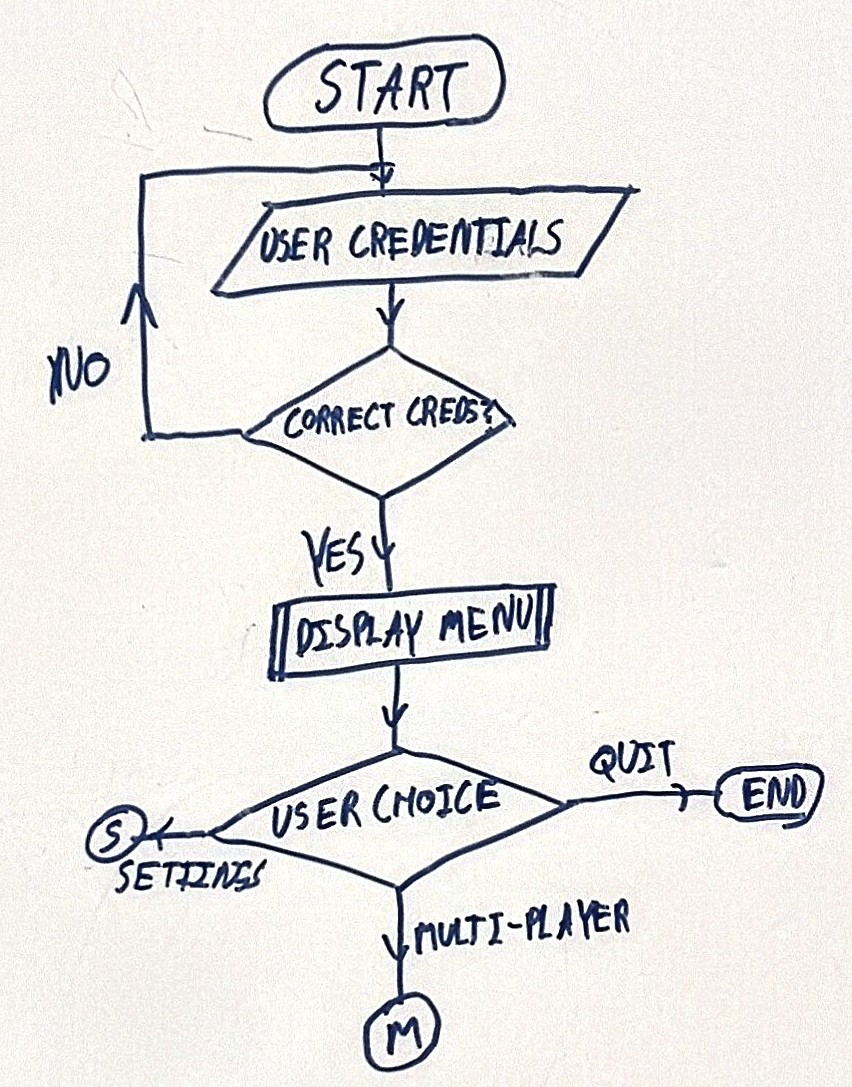
\includegraphics[width=1.0\linewidth]{Analysis/Images/Flowchart_Main.jpg} 
	\caption{Flowchart of main game structure}
	\label{fig:main_game}
	\vspace{-20pt}
\end{wrapfigure}

\vs
Currently, the player's interaction with the game is shown as below. The game will initially take the user's credentials in order to be able to authenticate the user. If the user has entered an invalid username or password, the game will show the original screen again, with a prompt telling them that they have entered the password incorrectly. If the credentials are correct, the user is moved to the main menu level, where they can select to change their settings, to join a multi-player game, or to quite the game. 


\vs
This will then lead to the other modules, which handle each component, and their flow charts are shown as well. This system is very familiar to most people and is quite logical, so there are not many possible misunderstandings. This makes it very effective at communicating to the user what is going on, and so serves its purpose well. Some games have hidden menus when the user clicks on play, such as offering different game modes, but many don't have a way of showing how popular each game mode is. This means that a user may click on a less popular game mode, and wait for a long time before a game lobby is formed.


\vs
There are many actions that a player can undertake, and all of these combined are called the game loop. This forms the basis of the game, and is what people are most interested in. The actions within most FPS games are very similar, such as movement, damage, death / re-spawn, score change, timer change, game end. 

\begin{wrapfigure}{L}{0.38\textwidth}
	\vspace{-20pt}
	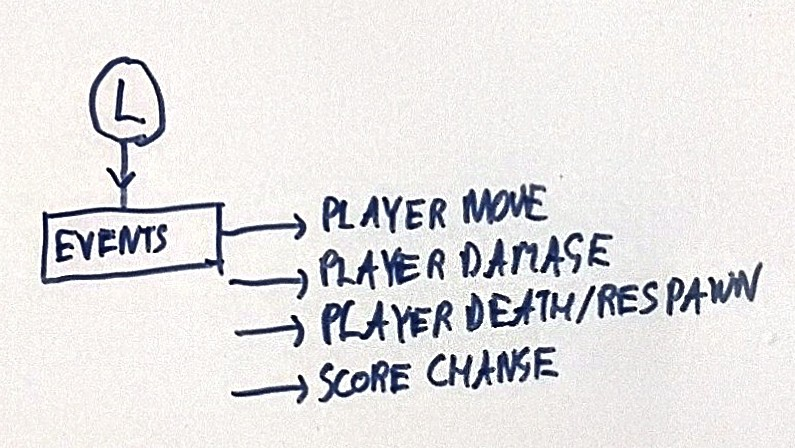
\includegraphics[width=1.0\linewidth]{Analysis/Images/Flowchart_GameLoop.jpg}
	\caption{Flowchart of the game loop}
	\label{fig:game_loop}
	\vspace{-15pt}
\end{wrapfigure}

\vs 
Each client sends a command to the server, indicating the move that has been played, and from that the server can apply those changes and replicate it to all of the other players, ensuring that everyone has a consistent version of the game state. The server is generally placed centrally amongst the players geographically, to ensure that all of them receive roughly equal latency which creates an even playing field. Additionally, once the game has finished, the player is shown an end screen, usually detailing their score, and their performance in the game, and then finally sends them back to the main menu, or gives them the option to play another game.

\vs
\begin{wrapfigure}{R}{0.3\textwidth}
	\vspace{-15pt}
	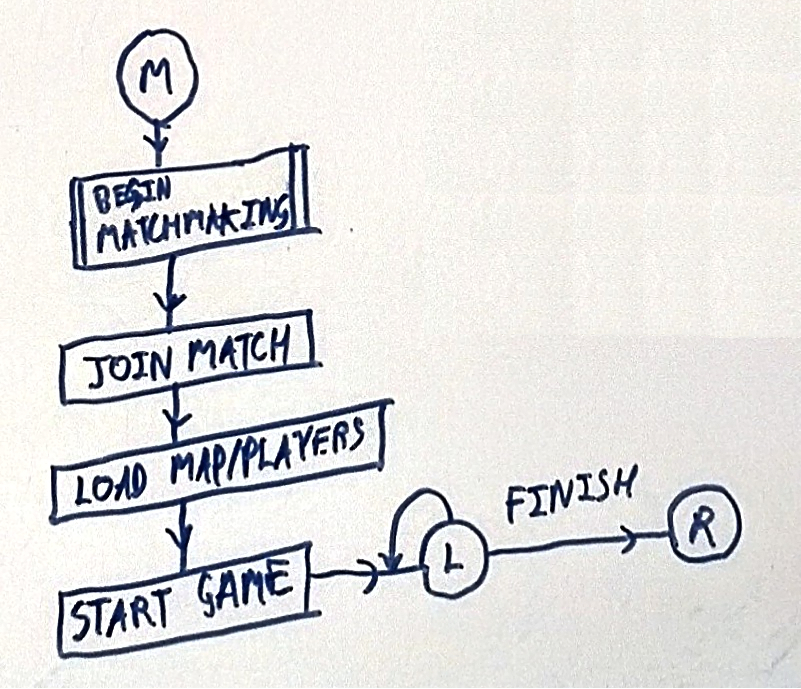
\includegraphics[width=1.0\linewidth]{Analysis/Images/Flowchart_Multiplayer.jpg} 
	\caption{Flowchart of the Multiplayer system}
	\label{fig:multi_flowchart}
\end{wrapfigure}

\vs
Once a user clicks on the multiplayer button, the begin matchmaking procedure occurs. This will allow for a the match to be found which finds a lobby of other players which is usually based on the latency between the player and the server, and any rating system that might be in place. Once this "lobby" is formed, they join a match, and the map and mode of the game is selected randomly. Then, the map is loaded locally on each user's device, and the players are loaded into the map, and the game begins. The game loop as shown above will cycle until one of the game's end conditions are reached, such as a goal limit, or a time limit. 


\vs
Once this happens, any rating changes are applied, and users have the ability to go to the main menu, or play another game. In many cases, the matchmaking procedure can cause long delays whilst players wait for a lobby of their current skill level to form. As a game loses active users, queue times can become much longer as there are just not enough people to fill a lobby, and eventually, people completely stop playing the game. 


\vs
This is obviously not ideal for players who are still interested, and therefore, it is essential that some sort of competitive bots are in place that will allow a player to still get the thrill of playing against people, but not actually require multiple active users to still be online. Additionally, as it is just the player, they can adjust game settings, timings, etc, to their liking, meaning they can find new ways to make the game fun again.

\subsection{Explanation of Choice of Project}

Firstly, a game that can be played on computer provides the best platform for a game, because it is easily accessible to most people, and provides enough computational processing power so that a more detailed game can be run. This however limits my audience to be mainly an audience of PC or laptop users. Additionally, the game will be written in PyGame, which is lightweight and does not require advanced graphics processing.


\vs
Hence, the game is portable, and can be played on a laptop without consuming lots of power. Furthermore, a computational solutions allows for some sort of AI to be implemented, which is almost impossible to do mechanically. This will allow for a much more immersive experience, and encourage people to play without requiring large time commitments. It is also better to run the game on a computer than a mobile device due to the larger computational processing which is possible. It would drain the battery of the user's device if they decided to play on a phone due to the large demands of AI based algorithms, especially neural networks.


\vs
There are multiple platforms to publish games on, such as Steam, and the Epic Games Store, which have very wide audiences, and this adds a sense of community to the game as well as allowing things like leaderboards to form, which will add more of a sense of competition to the game. This can mean that people are more willing to spend more time playing the game. Alternatively, I could create a website that people can access to download the game.

\vs
On top of this, it is generally much clearer to see what is going on when viewed on a larger monitor compared to a mobile device, and this is one of the things that was mentioned by stakeholders as will be shown below. This will also result in a more immersive experience that is more enjoyable for the users.

\vs
Additionally, using a computer will mean that there are more inputs available to the user. For example, from a computer, we have an entire keyboard which provides binary inputs, and a mouse which has further binary inputs in the form of buttons as well as an optical sensor which can provide a much more refined input and a scroll wheel which can be used to allow for quick changes.

\vs
On a phone however, this would be much more limited since any inputs would have to be in the form of touching buttons on the screen, which will take space away from the main content that is display. These buttons need to be clear in their meaning so that it is intuitive how the play the game 

\subsection{Stakeholders}

My stakeholders are generally all people who are too busy to play games during the week. I found these people through online forums, as well as friends who sufferred from similar problems. I sent them a survey to fill which allowed me to gain insight on what things they wanted to get from a game that would encourage them to play during the week. I further asked these people if they would be willing to download test versions of the game and play them and give feedback, which would allow me to consistently improve the game to my stakeholder's needs. The results of the survey are as follows.

\vs
\begin{figure}[H]
    \centering
    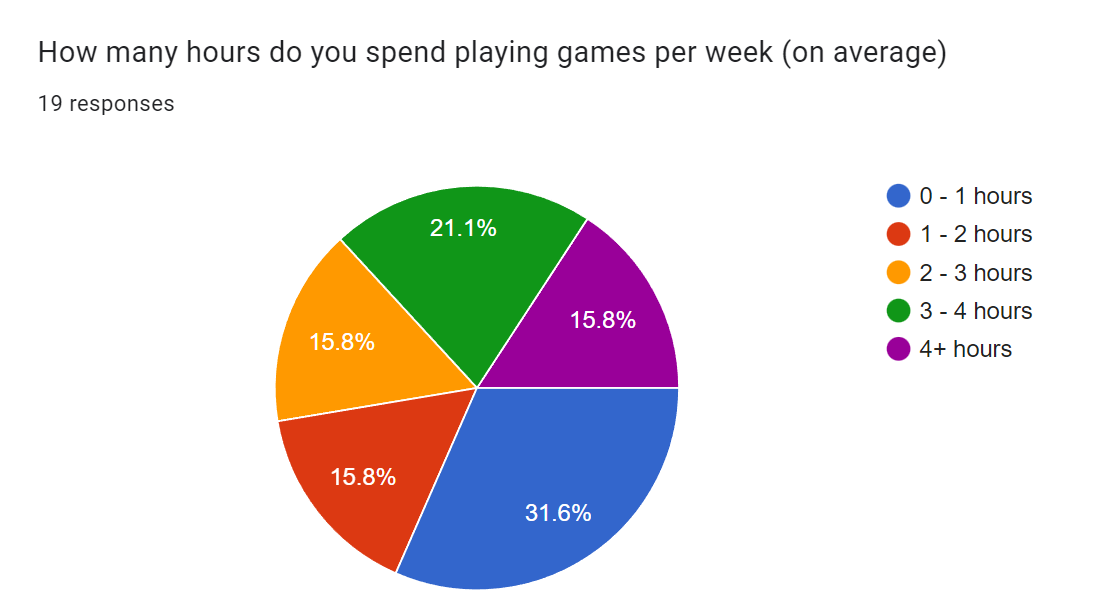
\includegraphics[width=10cm]{Analysis/Images/Analysis_HoursPlayedEachWeek.png}
    \caption{Number of Hours spent playing game per week}
    \label{fig:hours}
\end{figure}

This first question served the purpose of showing me the amounts of time that most people generally spend playing. About a third of people played less than one hour a week, and amongst the other sections, I observed that it was fairly evenly distributed. My game was primarily targeted at the people playing between 0 and 2 hours since this occupies about half of my sample, and is so there is definitely some demand for a game of this type, which focuses on shorter round times to accommodate more games.

\vs
\begin{figure}[H]
    \centering
    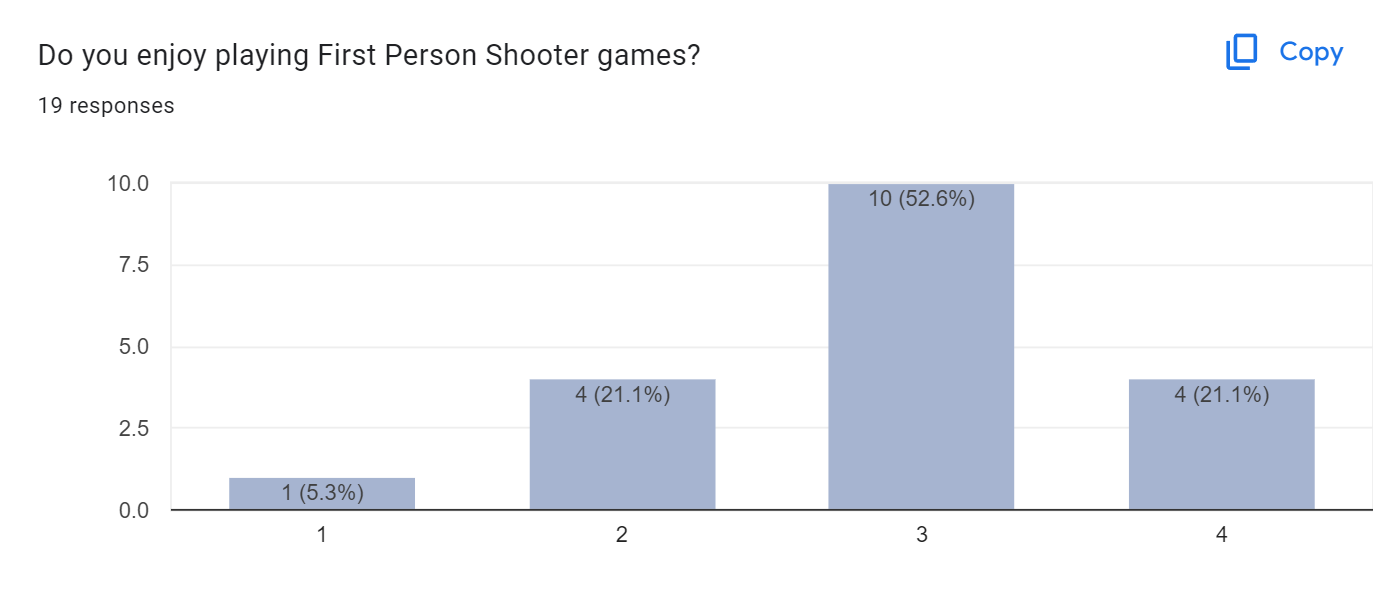
\includegraphics[width=10cm]{Analysis/Images/Analysis_EnjoyFPS.png}
    \caption{Enjoyment of shooter games}
    \label{fig:enjoyment}
\end{figure}

This next question aimed to find the proportion of people which either liked or disliked shooter games. This was important, since I wanted to build a game that people would still be able to enjoy, making them more likely to play in their spare time, or make time out to play it during the week. Additionally, this showed that not everyone likes shooter games, but this is perhaps to be expected.

\vs
\begin{figure}[H]
    \centering
    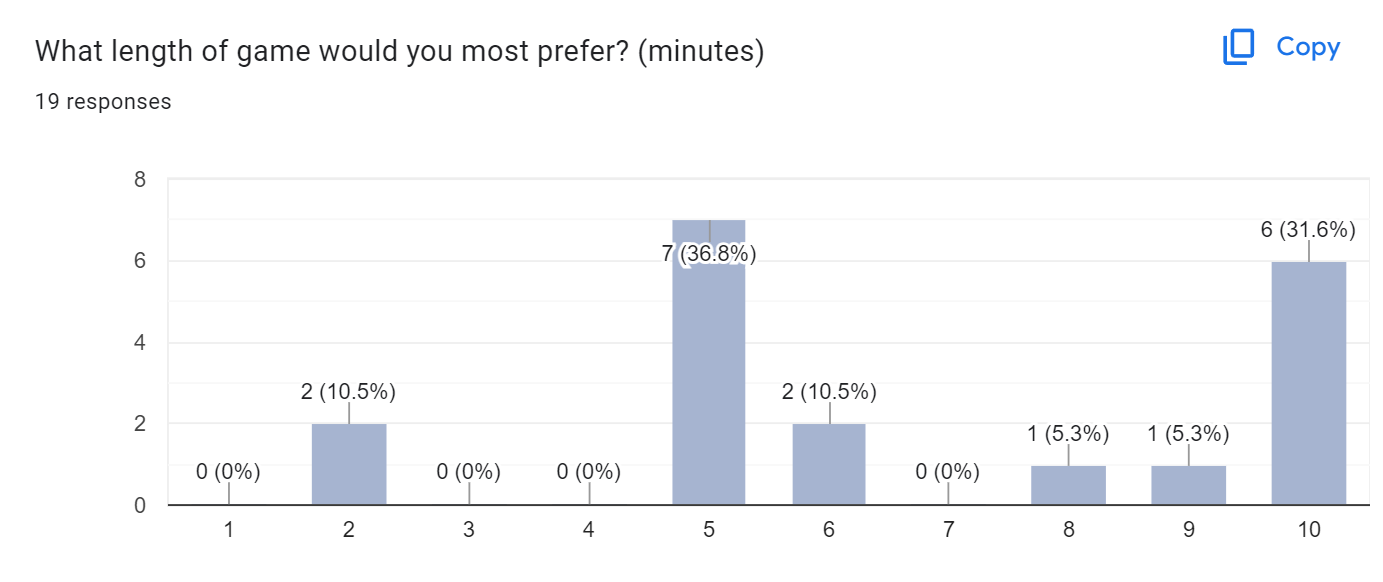
\includegraphics[width=10cm]{Analysis/Images/Analysis_GameLength.png}
    \caption{Desired Game Lengths}
    \label{fig:des_game_length}
\end{figure}

\vs
This showed me roughly how long I should make the rounds in the game. For the most part, the most popular responses were 5 minutes or 10 minutes, but there was some interest in even shorter rounds! In order to resolve this, it may be useful to allow users to set their own time limits in order to allow for variable length rounds, which is tuned to their style. This means that the game adapts to what people want from it, and means that they are more comfortable playing. For example, for some people it may not be possible to play multiple 10 minute rounds, hence they might choose shorter round lengths.

\vs

There were also other questions that were asked, but here is a detailed version of what they revealed. The other results were relating the factors that deterred people from playing during the week. The most common factors were work, school, and a lack of time. Additionally, when asked whether people avoided games with longer round times, 53\% said yes, whilst 47\% said no. The difference was a lot more noticeable however, when asked whether people wanted shorter round times in their games. Here, 58\% said yes, and only 42\% said no. The distribution of round times that people preferred had an average of 6.7 minutes, however, in order to accommodate a strict limit of 3 rounds, we will use 6 minutes instead. This survey provided a useful insight into what people would need to have in a game in order for them to be able to play during their schedules, and made it clear that there is a large audience for this type of game.


\subsection{Interviews}

In order to gain a better understanding of the needs of my stakeholders, I decided to interview them. I asked the following questions and got these responses back. These questions were linked to the questions in the survey but dove into more depth in order to get more information.

\vs
\begin{enumerate}[label=\arabic*)]
    \item Are you comfortable playing games during the week?
    \subitem If not, would you be more comfortable playing a game during the week if you knew that you could control how long you were playing for?
    \item What would be the requirements of a top-down shooter game if you were to play it?
    \item Would you be bothered if you were playing against advanced bots instead of real players?
    \item Would you like to be able to decide the length of your rounds?
    \item Would you like to be able to decide how long you want to play for?
    \item What things would make you more likely to play a game, or make time to play it during the week?
\end{enumerate}

\vs
\subsubsection{Interview 1: Sanjay}
Sanjay, my father, is working a full-time job, and doesn't have much prior experience with playing games. He does, however, play chess occasionally.
\begin{enumerate}[label=\arabic*)]
    \item No. Due to full-time work, I am extremely busy and so don't have the time to play during the evening. Also, having not played many games before, it is slightly daunting.
    \item I should be able to zoom out and find my location on the map, and navigate through it.
    \item I wouldn't be bothered.
    \subitem \textbf{Why not?} I don't want to wait for other players, and bots don't judge you for being bad. You can also choose the expertise of the opponents.
    \item Yes, of course
    \subitem \textbf{Why?} Depending on the time I have, I can setup the game
    \item Yes, a timer system would be nice, to restrict overall play time
    \item Shorter games, quick to setup, and it should be relaxing, not too competitive, and fairly easy to pickup
\end{enumerate}

\vs
\subsubsection{Interview 2: Vaibhav}
Vaibhav is studying robotics and AI at university, and is in a similar position to Moosa - not having much free time during the week. Therefore, he was a suitable stakeholder.
\begin{enumerate}[label=\arabic*)]
    \item No, since I don't have time.
    \subitem \textbf{Follow up:} If I knew exactly what time I would be spending, I would.
    \item Would have to have a great design, many features, many inventory items, like guns, shields, grenades, healables, being able to play with friends and view statistics
    \item No.
    \subitem \textbf{Why not?} Ultimately the game is to play against something. If I still get the dopamine rush, and still enjoy playing, then it doesn't matter. It doesn't present any hindrance. But give the bots random names.
    \item Yes I would like to.
    \item Yes that would be great.
    \item If I didn't have much work helps. Being able to play with friends is nice. Having some kind of ranking system and leaderboard would be great. Getting some sort of currency would be great.
\end{enumerate}

\vs


\subsubsection{Interview 3: Frank}
Frank is a student in my year, and is also very busy. He enjoys playing games, and so he was a viable stakeholder.

\vs
\begin{enumerate}[label=\arabic*)]
    \item Yes, I'd say so.
    \item Mainly good shooting mechanics, but good graphics would also be nice.
    \item Yes
    \subitem \textbf{Why?} Playing against real players is usually much more enjoyable. The bots would have to be very very good otherwise.
    \item Could be nice but probably easiest to switch between long and short games with less rounds at a fixed round length.
    \item Just an enjoyable game with a high difficulty ceiling
    \subitem \textbf{Would you consider a game which has an initially shallow learning curve?} This would make the game too easy and get boring quickly.
    \subitem \textbf{Would you consider a game where the bots get harder the longer you play?} If you can make the hard bots difficult to play against, then that's fine.
    \item A rank system would encourage me to play the game more, since it gives a feeling of achievement.
\end{enumerate}

\vs
\subsubsection{Interview 4: Jay}
Jay is another student in my year, and is also very busy. He enjoys playing games, and so he was a viable stakeholder.

\vs
\begin{enumerate}[label=\arabic*)]
    \item No
    \subitem \textbf{Follow up:} Current amount of stuff I need to do.
    \item I think it has to look nice, and be aesthetically pleasing
    \item That doesn't matter for me
    \item Yes, this sounds nice
    \item Yes, this would be very helpful. Perhaps a timetable so you can't play too early either, and a limit on how late too.
    \item If it involves some interesting mechanics. The week timer system would also be very helpful.
\end{enumerate}

\vs
\subsubsection{Interview 5: Moosa}
Moosa is currently studying engineering at university, and therefore is quite busy and so doesn't have much time to play games during the week.

\vs
\begin{enumerate}[label=\arabic*)]
    \item I don't really play video games anymore, since I don't have much time. I used to play a lot. I do play Minecraft but it is difficult since there aren't that many people to play with either.
    \subitem \textbf{Follow up:} Yeah probably. A social aspect of the game is quite important for me. I don't really play alone, I generally play with friends. If I knew that I could play with a group at a fixed time then definitely.
    \item A compelling story line and if not then multiplayer, different maps, wide range of weapons, different features, interesting mechanics, different game modes, like 1v1 and team matches.
    \item If it was me and my friends against bots that would be fine.
    \item That would be pretty useful. Some games go for quite a long time, so this a useful feature.
    \item This seems like a good feature, and being able to manage time is very helpful. Bad habits and overplaying is quite frequent.
    \item Obviously, popularity of the game helps. In-game interactions are quite funny. The social element of the game is the most important for me.
\end{enumerate}

\subsection{\textcolor{red}{Analysis of Interviews}}

We will look through each question in turn.

\subsubsection{\textcolor{red}{Question 1}}

Most people said that they were not comfortable playing during the week, primarily due to the amount of work that they had to do. This means that short round times, and preferably no queue times would be necessary in order to allow people to feel more comfortable playing games as a way of relaxing during the week.

\subsubsection{\textcolor{red}{Question 2}}

One of the things that was mentioned by users was that the design must be intuitive and easy to use, but also having reliable shooting mechanics that are fun to use. Additionally, almost everyone mentioned that it had to look aesthetically pleasing.

\subsubsection{\textcolor{red}{Question 3}}

Most people were not bothered by the idea of playing against bots instead of real people, although Frank did mention that he would prefer if the bots were good otherwise it would become boring quite quickly. Moosa also mentioned the idea of playing with friends against the bots would be acceptable as well.

\subsubsection{\textcolor{red}{Question 4}}

This was received well, but ultimately, it was not as important, since there was a global timer, but most people preferred having shorter rounds.

\vs
The overall constraint that people wanted was on the amount of time that they spent playing the game. Furthermore, people said that it would be a nice feature to have but not that it had to be in the game for them to play it.

\subsubsection{\textcolor{red}{Question 5}}

Everybody was very accepting of this idea and said that it was something that they would want in the game and would be a useful feature to have. Particularly, having short rounds and then a global timer seemed to be the preferred option.

\vs
This also would help them to solve the problem of having not enough time to play during the week, since now they can limit themselves to only play for a limited amount of time.

\subsubsection{\textcolor{red}{Question 6}}

People mentioned that they would be more likely to play a game during a week if there was some kind of ranking system or a leaderboard of some kind.

\subsection{Stakeholder and Public Requirements Summary}

Here is a list of all of the stakeholder's requirements from my game so far, as well as some things that will improve overall user experience. These were compiled from the interviews, and are justified in the table below.


%\begin{longtable}{|p{4cm}|p{11.5cm}|}
\vs
\begin{center}
\begin{longtable}{|p{4cm}|p{11.5cm}|}
    \hline
     Requirement & Justification\\
    \hline
    \hline
    Shallow Learning Curve & The game must be easy to learn how to play, without requiring a large time investment, which makes the game much more fun to start playing, but must get difficult at some point. This can be enforced by making the mechanics easy to understand and keeping interactions simple.\\
    \hline
    Short queue times & The game must have very short, or no queue times to play, which means that the users can spend more time playing instead of waiting. This was brought up quite frequently in the interviews with stakeholders.\\
    \hline
    Clear UI & The UI must allow the user to understand what each thing represents without too much difficulty. This makes the game more "inviting" to play, and so therefore encourages people to play more.\\
    \hline
    Login System & The project must be able to store user data, such as games played and games won, as well as their login credentials. This will allow them to track their progress and view statistics about their account.\\
    \hline
    Data Security & The project must store this data securely, and allow for logins to be efficient.\\
    \hline
    Leaderboard & The users must be able to view the leaderboard and their position on the leaderboard relative to other players in different categories, such as games played, games won and level.\\
    \hline
    Movement mechanics & There must be a variety of movement mechanics in order to keep the game interesting, and these must be practical to use in game.\\
    \hline
    Time Management & Users must be able to control the amount of time they want to play the game for, and how long the rounds are. Furthermore, players must be able to see how long they have left in a given round.\\
    \hline 
    Gameplay & There must be shooting mechanics, movement, and power-ups that make the game more versatile and interesting to play.\\
    \hline
    Graphics & The game must be visually appealing, or at it should at least be easy to decipher what is going on.\\
    \hline
    Multiplayer & This would allow people to play with friends and would make playing the game more enjoyable and immersive. This is a standard feature of most modern games and would be expected from stakeholders.\\
    \hline
\end{longtable}
\end{center}

These will be taken into account when constructing the design and development of my project.

\subsection{Overall Analysis and Problem Statement}

From all of the analysis done so far and the data collected, we can create a concise summary of it here. This will highlight key points we need to consider, and then we can write a final problem statement, which we can follow.

\vs
Firstly, we saw that the time constraint on people was one of the major restricting factors from them playing games. Having shorter rounds, or allowing people to select the round length would allow them to play games at their convenience, since many games that they may enjoy may have round times that are inconvenient to their schedule and therefore are deterred from playing entirely. The most popular round times were 5 minutes or 10 minutes, so it may well be that I create a system that allows people to select the round time before the round starts. This will be more thoroughly investigated in the Design section of the project. Additionally, I saw that a lot of people enjoyed shooter games, and so this was a safe option for the genre of game, since it would almost certainly guarantee that there is an audience for it.

\vs
Furthermore, I noticed that people didn't enjoy having long queue times since it meant that they would waste a lot of time looking for a game rather than playing. However, this is a universal problem with any multiplayer game, and so it is almost necessarily going to have to be a single-player game, using some sort of algorithm to create an agent that can make "smart" decisions about how to play the game. This will mean that we can add a difficulty setting which will let the player decide which types of bots they would like to play against, making the experience more interactive for the user.

\vs
On top of this, there will be a leaderboard and rank system which be based on the games played and the games won, as well as the score accumulated through playing. This will let the player feel a sense of achievement and this was pointed out by a few of the stakeholders I talked to before. This will be available through the game and users will be able to see where they rank on the leaderboard and how many points they have.

\vs
\textbf{Problem Statement: } The aim of the project is to create a top-down shooter game, named Momentum, which will allow people to play according to their schedules, and let them play against AI bots. The game will allow them to decide how long they want their rounds to be and how long they want to play for overall. They will be able to move their character in different ways, and shoot enemies to increase their score, and the team with the higher score wins.


\subsection{Requirements of the Solution}

The solution must have short queue times, and short round times, ensuring that the player will be active for as long as possible, encouraging them to play further.

\vs
The most common comment on what factors deter people from playing during the week was time commitments, and so it was essential that the game prioritised quick game times, and fast matchmaking, in order to maximise the time that the player is active playing rather than waiting for a game to start.

\vs
In order to solve this, we will use artificial intelligence to create "bots" who can fill lobbies if they are not filled sufficiently quickly. This will allow for games to start as soon as possible, and reduce the amount of time people must wait before a game starts, hence making them more likely to play the game. This promotes starting a game, because the amount of time between pressing the play button and joining a game is shorter, and so people are more inclined to start new games, because they do not take as long to find. Additionally, this will still give the players a feeling of playing with other people, even though they are not.

\vs
Shorter rounds ensure that there is less at stake, and that many rounds can be played in a shorter period of time, and so each game does not feel like as much of a commitment and therefore leaving a game does not have as much of an affect on the player. Additionally, there is no pressure of being judged by other players, or ruining another player's game, since there are just bots playing on the other side, so people will be more likely to judge when they should start and stop playing.

\vs
Additionally, the game will include fast-paced mechanics in order to allow for more intense rounds, which will mean that players see more action in a shorter period of time. There are very very few games which are left in this niche, as many games and franchises, have made their games slower and more tactical. The mechanics within the game will be things just as dashing, sliding, etc. This will allow players to move across the map even faster, and due to the open map design this will be much more easily accomplished. 

\subsubsection{\textcolor{red}{Hardware Requirements}}

In order to run the AI on the machine, the computer must have a CUDA-enabled graphics card. This is quite a steep limitation, but it is available for most people, and so shouldn't be a problem. Furthermore, the computer must have a monitor, keyboard and mouse, because there are the inputs and outputs that are most commonly used and therefore our game will also process using these.

\vs
Additionally, it will need to have at least 4GB of RAM in order to house all of the AI models and all of the data that goes alongside the game. This is necessary, since AI is a key part of our game and we have to load it into memory otherwise the game would be completely unplayable.

\vs
\subsubsection{\textcolor{red}{Software Requirements}}

In order to run the code, the user will need to have CUDA installed, which will allow the neural network to take advantage of the massively parallel architechture of the GPU. This is important as we want to minimise the amount of time it takes to use the model to produce an action. 

\vs

Furthermore, since the game will be written in Python \verb|3.10|, the device must have this version of Python installed, otherwise the game will not operator properly. Additionally, all of the libaries that will be used in the game's final code must be installed also. This is absolutely required, since otherwise the project would take extremely long to complete without libraries, and often libaries have been tested and optimised repeatedly, thus offering a significant performance advantage over raw Python code.

\subsection{Justification of Computational Methods}

The use of computational methods here is paramount. Using a computer will allow us to do multiple things, such as creating an AI which can play with the players. This will require parallel processing in order to achieve smooth gameplay and rendering, as there will be multiple bots which are interacting in the game. Obviously, a reinforcement learning model or similar cannot be done by hand, and so a computer must be used in order to allow for an interactive experience.

\vs
This problem is solvable by computational methods, and is best suited to computational methods, because it is quite difficult to find people to play with in the real world, and they may not be interested, or available to play at that time. By using computers, we can use bots for the person to play against instead of waiting to be connected against other players to play a game. This also the player to dictate the length of the game as well as any game settings they may wish to change. This results in a much more versatile experience for the player and will likely keep them engaged for longer.

\vs
Additionally, we can use computational methods such as abstraction in order to aid the development process. We will examine each in turn.

\vs

\subsubsection{Abstraction}

Abstraction will be used in order to create flowcharts and pseudo-code which will layout the underlying structure of the code. This will allow us to much more easily convert this into the final program, and also mean that we can spot any potential errors before finalising it into code, which will reduce the amount of time we spend debugging our program.

\vs
Furthermore, we will be using external libraries in order to add some abstraction to the graphical and hardware elements of the project. For example, many machine learning libraries are very inefficient to run on a CPU so will use low-level hardware interfaces like CUDA to speed up the process with GPUs which utilise parallelisation in order to do operations like matrix multiplication and addition many times faster. On top of this, a library like PyGame will allow me to focus on the core aspects of the game instead of also having to worry about the implementation of the graphical processing of the game. This adds some abstraction to the game since I no longer have to worry about these things, and it is now hidden by the veil of other classes and methods that have already been tested thoroughly, which means I also can reduce the amount of testing that needs to be done.
\vs

Furthermore, abstraction will be useful as it will allow us to remove details which are irrelevant, and focus on the important attributes and procedures that we need to implement. For example, for a button, we don't need to know what the button does specifically, only that it has a shape, colour, position, and text written on it, and that we want to be able to detect if we are clicking the button at any time.


\subsubsection{Decomposition and Modularity}

Additionally, we will be using classes in the game in order to create a modular program which is much easier to test as we go, and easier to debug. This is useful, since now we can create multiple instances of the same class, such as the player and enemies instead of having to create a number of instances manually. This also allows the game to be more versatile, since we can quickly change singular elements of the game, without having to alter the whole program. This could happen, for example, if users are giving feedback that the game needs changing. It also makes it easier to test and debug, since we can now test each class independently of other classes, and focus on their individual implementations.

\vs
Another way we will be using computational methods is to decompose the problem into smaller, more manageable problems. In this case, we can use the class structure to make the problem much easier to visualise, and code small components of the project. For example, we can work on just the player movement, or the weapons system individually of each other, and then combine them at the end.

\vs

\subsection{Limitations of Proposed Solution}

My main limitation is likely to be hardware. This is in two stages. Firstly, during training, which is done locally on my machine, I will need to use a GPU in order to get a reasonable completion time, as training of AI models can often take hours, or even days. Furthermore, when the player is playing the game, they will be running a model which controls 5 agents, and obviously, this is not an easy computational task, and so it is essential that a GPU is used, and that the game is well-optimised. This can be done using the CUDA library, and the GPU version of PyTorch.

\vs
Additionally, my game will be limited to 2D because I am using PyGame, and so any game that I do make will need to be either top-down or side-on. This means that I will need to use images as my graphics, and potentially use multiple images and cycle through them in order to create the illusion of animation. 

\vs
On top of this, another problem that may potentially arise is that people may not know how to run Python programs, or not have an NVIDIA GPU which is what many modern machine learning libraries run on and is likely what my project will also use. Therefore, it is important to create a list of system requirements for the game that is accessible to most people, and if a GPU is not available the program must be able to run somewhat efficiently on a CPU, which may be challenging. Additionally, packaging the program into an executable file will make it much easier to use for most people, since no specific requirements are needed if it is packaged, except for the platform, but we can package specifically for each platform if needed.


\subsection{Success Criteria}

In order to be able to evaluate the success of my project, I created a list of measurable success criteria that would be able to objectively ensure that the features that were required by the stakeholders would be met.

\vs
These were found using existing computational solutions and the research done by interviewing stakeholders, which we covered before.
\vs


\begin{center}
\begin{longtable}[c]{|p{2.7cm}|p{6.7cm}|p{5.7cm}|}
    \hline
    Name & Success Criterion & Justification\\
    \hline
    \hline
    Gameplay Length & Allow the user to set the total amount of time they would like to play for. & This will let people decide how long they want to play for, and make it so that they can set the game to be as long as is enjoyable for them.\\
    \hline
    Movement & The player can walk around the map, rotate, and cannot pass through other players or objects. & This will make the game more realistic and intuitive to play, since most games already have collisions in them.\\
    \hline
    Player Login & This will let players enter their username and password, which will be checked against the entry in the database. If the login details are correct they will be able to view their profile and play games. & As mentioned before, this will encourage players to play more often, as there is a sense of progress in the game, which makes it more entertaining to play.\\
    \hline
    Rating System & There will be a rating which will be visible to the user and is updated at the end of every match based on the Elo rating system as well as how they performed in the game. & This will further add to a sense of progress, and will provide us with a way to construct leaderboards and things of that nature. Furthermore, it encourages players to get better at the game.\\
    \hline
    Weapon System & The game will contain several different weapons: Assault Rifle, Sniper, and Shotgun. These will each function differently and have different behaviours. & This will add more variety to the game and allow the players to have a better experience.\\
    \hline
    Database System & The database must hold the following information in 3NF.
    \begin{enumerate}
        \item Username, Email, Password
        \item Player Level
        \item Player Experience
        \item Matches Won
        \item Matches Played
        \item Matchmaking Rating (MMR)
    \end{enumerate} & This will allow the user to track their progress, and this will give them a sense of achievement. This encourages the player to play the game more, or make more time to play it during the week.\\
    \hline
    Leaderboard System & There will be a global leaderboard which will show users where they rank in the player-base based on their ranking, and will also show the top 100 or so players of the game. People will be able to search the ratings of other players as well, for example, friends. & This will add a sense of competition into the game and for the players in the top 100 will add an added sense of achievement and further competition to reach rank 1. Furthermore, this will add a bit more of a social element to the game as this will allow people to view what rank their friends are at, and they can compete against each other.\\
    \hline
    Bots & There will be bots which allows for players to play against them even if their friends are not online to play against. These bots must be able to play to a standard such that a human player would not be able to discern between a human and a bot. & This will solve a large part of the problem that people have with currently playing games, namely, a lack of time. Therefore, implementing this feature will allow people to play according to their schedule and convenience, which is a desirable feature as seen in the interviews.\\
    \hline
    Menu System & There will be a menu system that will let a player exit the game, set a timer, and create a game. Within the timer settings, the user can choose how long they wish this timer to be. Within the game creation menu, there will be options for the difficulty of the bots, the length of the rounds and the number of rounds. & This is a useful criterion for success of the project, as many people mentioned that they would be more willing to play if they knew that they would be able to control how long they are playing for, and not play for too long.\\
    \hline
    Difficulty Selection & The player must be able to choose the difficulty of the bots that they are playing against, and playing with. & For players that are less experienced, they can play with better team-mates and worse opponents in order to learn more about the game, and once they are more comfortable can play against better opponents.\\
    \hline
    Game Loop HUD & In the game loop the player must be able to clearly see the team scores, and the time left in the round. & This is important since the player's decision will be guided by the time and score of both teams.\\
    \hline
    Inputs & The user must be able to give inputs using their keyboard and mouse depending on the context. & This is the most commonly available input for a computer or laptop, and therefore, this is the input that our game must be compatible with.\\
    \hline
    Menu Screen UI & The menus must contain clickable buttons which are clearly labelled and will direct the user where they are supposed to. & Buttons are very intuitive to use and will mean that the user can understand what their purpose is when clicking on them. The menu must have buttons, since this is the most common way to interact with a game, and can be easily adapted for other inputs types in the future.\\
    \hline
\end{longtable}
\end{center}

%\clearpage
%Remove bg from flowcharts
%Long table package
%Testing even pretty basic things   
%Include mistakes
%Make mistakes -> J. Savage
%pythonstruct
%show each stage

\clearpage
\section{Design}
In order to be able to write the program, we need to break down the problem into smaller problems, which are much easier to address, and link them together to create the final product.
\vs

I have created the following table highlighting the different sectors involved within the project.
\vs


\begin{longtable}{|p{4cm}|p{11.5cm}|}
    \hline
    Section & Purpose\\
    \hline
    \hline
    Base & This will contain the basics of the \m{Player} class, such as the hit-box, position, and collisions with the map.\\
    \hline
    Gameplay & Controls the length and state of the game, and will be responsible for display winners, managing teams and tracking player scores. Additionally, it will also control the game mode being played.\\
    \hline
    Weapon & This will have a base class and derived classes for individual weapons, and its methods and attributes, such as ammo, reloading, and weapon switching.\\
    \hline
    Database / Account Management & This will be done in SQLite as it is a lightweight database. Alongside this, a login system can be made, where the server is run on a web server. This is linked to the UI, which will allow users to enter their details and login.\\
    \hline
    UI & This will allow users to navigate the game, start games and login.\\
    \hline
    AI & A large part of the game will be AI. This will ensure that a player can join a game immediately and not have to wait for a queue. The player will be able to select different levels of difficulty.\\
    \hline
\end{longtable}
\vs

Here is a top-down diagram showing all of the different sections of the project. We will break down and discuss each section individually in depth, as well as justifying why these modules are necessary.

\begin{figure}[H]
    \centering
    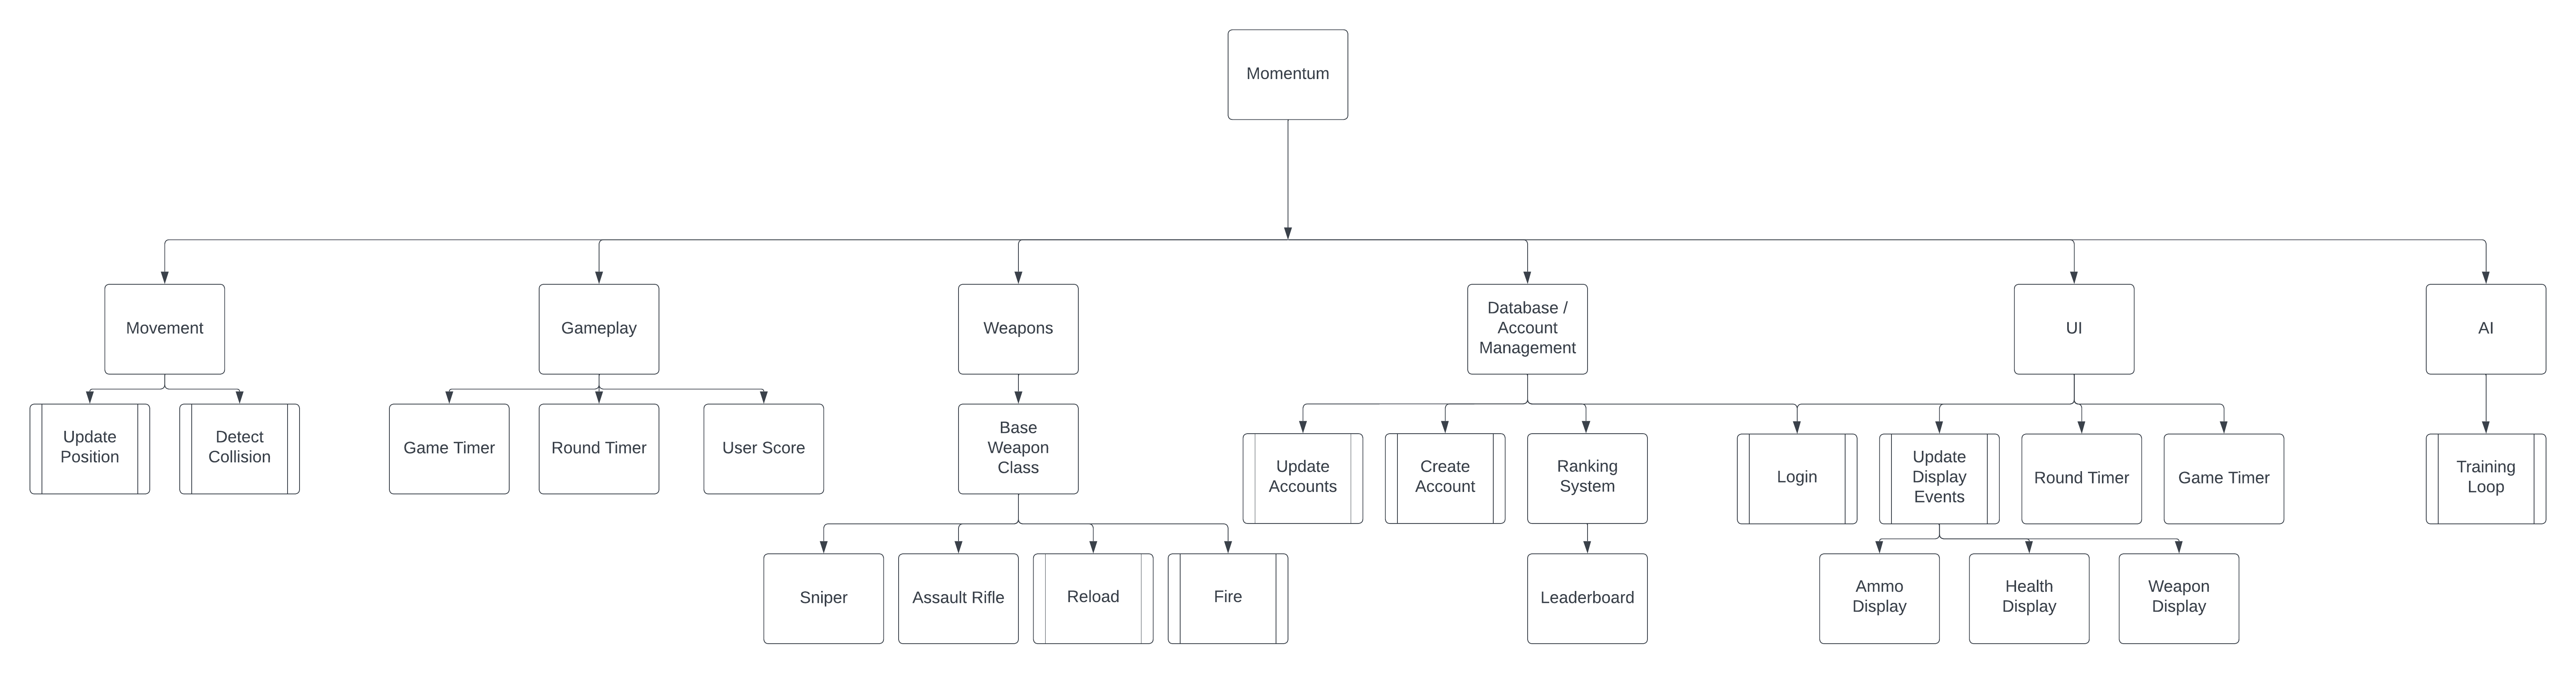
\includegraphics[width=15cm]{Design/Images/TopDownDiagram.png}
    \caption{A top down diagram of the project}
    \label{fig:td_diagram}
\end{figure}

In consideration of all these features there are few different languages and frameworks which come to mind as being suitable for the job. These are Unreal Engine, Unity, and PyGame. We will evaluate each one in turn.

\begin{longtable}{|p{2.8cm}|p{1.6cm}|p{5cm}|p{5cm}|}
    \hline
    Framework & Language & Pros & Cons\\
    \hline
    \hline
    Unreal Engine & C++ & \begin{itemize}
        \item Extremely performance orientated
        \item Supports OOP
        \item Has Learning Agents library (PPO)
    \end{itemize}
     & \begin{itemize}
        \item Not familiar with C++
        \item C++ is difficult to write and maintain compared to others
        \item Platform dependent
        \item Very hardware intensive
        \item Better suited to 3D games
    \end{itemize}\\
    \hline
    Unity & C\# & \begin{itemize}
        \item Also supports OOP
        \item Platform independence (bytecode)
        \item Implements MLAgents 
    \end{itemize} & \begin{itemize}
        \item Not familiar with C\#
        \item Lot of framework specific knowledge required
        \item Learning algorithm cannot be modified as much
    \end{itemize}\\
    \hline
    PyGame & Python & \begin{itemize}
        \item Very familiar with Python
        \item Many ML libraries in Python
        \item PyGame is much simpler than Unity and UE
        \item Platform independence
        \item Supports OOP
    \end{itemize} & \begin{itemize}
        \item Python is significantly slower than C++/C\#
        \item PyGame lacks lots of functionality that others provide
    \end{itemize}\\
    \hline
\end{longtable}

Based on all of these, I have chosen to go with PyGame for my project. 
\vs

\textbf{Justification:} This is because it provides the best flexibility and means that I do not have to work within the confines of a game engine that I am not as familiar with. This will allow for a much more controlled environment, and I have a lot of flexibility in how the game is implemented.

\vs
Additionally, PyGame is still relatively light, so despite Python being slow, it is possible to still get a 2D game running at 500-600 frames per second, and so even with more load placed on the system it should still be relatively quick.

\vs
One library that may be very useful to us, is \m{Cython}. This is a Python library which allows for Python files to be compiled into C, and then executed at runtime at a much faster speed thanks to C's performance.

\vs
However, this does have one caveat that the game code will have to be recompiled each time I want to make a change. Therefore, it makes the most sense to compile the game code at the very end when we have finalised all of the aspects of each class. This will provide a much more stable environment to work with and mean that I am not excessively recompiling each time I want to check whether a change has worked.


\tbr

\subsection{\textcolor{blue}{Game States}}

We will need several classes in order to run the game effectively. The first one is the \m{Game} class. This will control the whole application and contains the loop from which all other functions are called. This is justified because it allows us to encapsulate the entire application into one project, and we can have modules within it. It also makes certain things easier, such as managing all of the different states.

\vs
Then, we have the game state manager. This is effectively going to let us get and set which state we are in currently, and allows us to change it from within menus and other states. This makes it much easier to process and understand the game. This is justified because it gives us a centralised way to edit the current state in the game. This is useful because it means that we can move between states easily, and we can define this behaviour according to what we have done, just as clicking buttons in the menu, or pressing certain buttons.

\vs
\begin{longtable}{|p{3cm}|p{5cm}|p{7cm}|}
    \hline
    State & Explanation & Justification\\
    \hline
    \hline
    Start & This will be the main menu of the game, and will allow us to create a game, options, set timer, and exit game. & This is the main interface through which the user will interact with the game. Therefore, we need to have this in order to allow a user to intuitively interact with the game.\\
    \hline
    Options & This will be the options menu, containing things like keybindings. & This is important because it allows the users to customise the game to their standards and this makes it more enjoyable for the player, since it is to their liking.\\
    \hline
    Login & This will let a user who already has an account to submit their login credentials and will then verify these details. If they are valid, they are redirected to the start menu. & This is important because we need to have some way to track user progress in an accurate way, and so we also need to keep this in the game's state in some manner.\\
    \hline
    Register & If the user does not already exist, it will allow them to create a new account using an email address and password. & This will allow the user to be able to track their progress, which is quite important for some people, since it gives a sense of achievement.\\
    \hline
    Create Game & This will let the user create a game. & This is important since otherwise the main game loop would be inaccessible to the user, thus making my project redundant.\\
    \hline
    Set Timer & This will allow the user to set how long they would like to play for in the entire session. & This was one of the things that was mentioned by the stakeholders as being very important to the project.\\
    \hline
    Game Loop & This will be the place where the user will spend the majority of their time. This will run the main game and will be the main attraction of my project. & This is a game state because we need to be able to shift between this and the other game states and menus.\\
    \hline
    Game Over & Once the player's time is over, or the round is over, the user must either be forced to exit the game, or to start another round if they still have time.& This exists as it also shows the outcome of the game and provides a nice way of concluding the user's experience without making it too abrupt.\\
    \hline
\end{longtable}

We will need to pass values between the game states in order to allow things like global variables to exist in the game state. This will contain things like player settings, PlayerID, and the amount of time left until the game will close itself.


\vs
There are a few possible \textbf{data structures} that we could use to transmit return values between different states. These are dictionaries, classes, and lists (linked lists and arrays are modelled as the same thing in Python.)


\vs
We will be using a dictionary to transfer these return values, because this is the most convenient and versatile format that will allow us to transfer data between states in a way that is maintainable. The other options that we have available to us is a class or a list.

\vs

\subsection{\textcolor{red}{Game Loop}}

We need to create a base of the game loop and will house all of the mechanics which are relevant to the game, such as the time left in the round, the score of each player, the position of each player, etc. This is important since we need to be able to track all of these statistics as we will need to update the user's profile after the game is over.

\vs
Firstly, we will define the processes and events which take place in the game loop.

\begin{longtable}{|p{3cm}|p{6cm}|p{6cm}|}
    \hline
    Event & Explanation & Justification\\
    \hline
    \hline
    Movement & This will allow the player to move and control their character on the screen. The player will move relative to the world. & The game relies on players interacting with each other which is only possible if they are able to move. The AI will use this movement and input system to simulate a real player but this will be fed into the inputs for another instance of a character.\\
    \hline
    Time Tracking & We will show the amount of time left in the round, and how much time they have left in their play session. & This was one of the features that appealed to a lot of the people that I interviewed. Having this feature will let them control how long they are playing for and to not exceed that.\\
    \hline
    Score & This will be updated every time someone makes an elimination, or is eliminated. & This will be used to update the ranking rating at the end of the game, so is essential to track accurately. During training this will be used to monitor rewards to train the model.\\
    \hline
    Weapons & Will look for events to fire weapons, and will check for any intersections between rays and players. This will then be used to update the ammo of the player and the health of the player if one is hit. & This is essential to the game since we must be able to interact with other players, and eliminate them in order to move the game forward, and to allow players to gain a score.\\
    \hline
    Rendering & The player will need to be able to see their character and HUD, but this is not relayed to each of the bots, and so therefore, this needs to be done independently of the current game. In other words, we take input from the state of the map right now, but the player's view does not interfere with the game's progress. & If the user cannot see the screen, then they will be unable to play the actual game. Therefore, is essential that the game is rendered accurately and consistently.\\
    \hline
    Collisions & We need a way of reliably tracking where players and whether they are colliding with the map or not. & This is important since otherwise, the game would be very dull and this adds more complexity to the strategies possible.\\
    \hline
\end{longtable}

\vs
We will have the player on the centre of the screen. We know the dimensions of the screen we are drawing, so for efficiency, if a player is not within those dimensions, we will not draw them, but they will still exist. We can do this, by calculating their relative positions to the player, and then translating to this to where they should be on the screen. We can do this with the formula shown below.
\begin{align*}
    x_\text{screen} &= x_\text{object} - x_\text{player} + \frac{x_\text{width}}{2}\\
\end{align*}

A similar expression is produced for the $y$ direction. We can calculate these co-ordinates for each object and then rule out those where the $x$ or $y$ ordinate is not on the screen. In the initial parts of the game's development, we will ignore this, and just render the whole map.

\tbc

\subsection{\textcolor{blue}{Movement}}

In order to create forwards and backwards movement, we just simply apply a multiple of the forward vector to the character. When the player presses W they will be moved forward, and when the player presses S they will be moved backwards. This is justified as this is the standard for most modern games, and so will be what most people are familiar with, hence making the game easier to start learning.
\vs
\vs
In order to rotate the character, a mouse will be used and the position of the cursor from the character will determine the angle which the character faces. This is justified because this will be the only way of allowing the user to accurately rotate the character where they want, since the only other common input is a keyboard, but this has binary readouts which will not allow the user as much control as they would with a mouse, which provides a much more refined output. This is then the angle at which any shooting is done, and the movement vectors will stay consistent with the direction the player is facing. The player will see a rotated player, and the world will stay in the same direction on the screen. This is justified because it allows for a much more intuitive experience. 
\vs
\vs
We can find this angle using the following formula, where we use $(x_0, y_0)$ to find the centre of the screen, and $(x_1, y_1)$ to represent the position of the cursor. Then, the angle below the horizontal line is $\theta$. If $\theta$ is negative, this just represents it points above the horizontal line. We will not run the code if the cursor is at the centre since otherwise this would return an infinite value. In that case, we can manually deal with the cases. We can see that if the cursor is below the centre of the screen then we must point downwards, and vice versa. We can justify using this formula since it is optimal for our application, as it has a constant complexity, and other ways that are not formulaic must have a larger time complexity. In a game, optimisation and efficiency are very important and so it is key that we use this formula to reduce computation time per frame, which is essential, since we are going to be using this formula very frequently.
\vs
\vs
\begin{align*}
    \tan \theta &= \frac{y_1 - y_0}{x_1 - x_0}\\
\end{align*}

\vs
The shift button will be used to dash which will move the player very quickly across the map, and will be put on a cool-down. This will be done by adding a sudden acceleration to the character in the direction they are currently moving, and then removing this acceleration, and decreasing the speed drastically. This effectively creates the illusion of dashing or jumping which is what we want to achieve. This is a justified 
\vs
\vs
Additionally, we will need a procedure to calculate position. We will set an initial position for each player. This will be where they spawn into the game initial, and where they respawn after each death. We will need to create an initial direction vector as well, in order to preserve the orientation of the player relative to the map.
\vs
\vs
There are two aspects to the development of the game. The first is the underlying framework which handles the "back-end", such as physically moving the players on the map, firing projectiles, detecting collisions, and tracking scores. Then, we have another section which handles the user's point of view of the game, such as the menus, the camera which tracks the player's character, and the UI.
\vs
\vs
Hence, in the development, we must consider the back-end of the project first, since this will allow us to train AI, who don't have a front-end to the game. The reason for this will be shown in the AI section.
\vs
\tbr

\subsection{\textcolor{red}{Weapons}}

There will be one parent weapon class which will contain all of the common methods and parameters that each weapon will take, such as handling ray casting to detect collisions with objects, and then further to see whether damage should be dealt to it. From this, individual weapon classes will be created which will allow for individual weapon categories to be made and customised, which players will then be able to select at the start of a game.

\begin{enumerate}[label=\alph*)]
    \item Assault Rifle
    \item Shotgun
    \item Sniper Rifle
    \item Sub-machine gun
\end{enumerate}

The base class will be as follows.

\vs
\begin{tabular}{|p{4cm}|p{11.5cm}|}
    \hline
    Attribute & Purpose\\
    \hline
    \hline
    Direction Vector & This will be a unit vector pointing in the direction that the player is facing.\\
    \hline
    Ammo & We will store the maximum ammo in each cartridge and the current ammo. This will be deducted by one each time we fire.\\
    \hline
    Firing & Each time we fire the weapon, we will create a ray which can be traced to detect collisions with the enemy players.\\
    \hline
    Reloading & This will cause the weapon to be unable to fire a period of time, but refills the ammo in the weapon.\\
    \hline
\end{tabular}

\subsubsection{Firing Procedure}

We need to be able to fire a projectile in the direction of the weapon. We set the source to be the centre of the player. We will then create a sprite centred at the source and will have a constant velocity in the direction of the of the weapon (the player's forward vector).

\vs
We will need to create a way to detect collisions between rays and blocks and between rays and players. We will then take the closest of the two collisions to be the "dominant" collision, in other words the collision which we will need to focus on primarily. If this collision is with another player, we will need to check whether they are on the enemy team or not, and if they are then we need to deal damage and award some points to the firing player, and otherwise, we do nothing.

\vs

\subsubsection{Collision Detection}

As mentioned before we need a way to detect collisions between a ray and an object. There are multiple types of collisions that we need to be able to detect and handle. In this case, the primary one is a collision between a line and a circle. We will be using vectors in our program, since this will let us quickly and effectively find collisions and use vector methods and properties which are much easier to work with than Cartesian equations.


\tbc
\subsection{\textcolor{red}{Database / Account Management}}

To do this, there is a class in the Unreal Engine framework that will enable me to connect the game to a database. This will be stored on a central server so that no user can access it directly, and a login page will be created. This login page will take a user's player name and password, hash the password locally, and transmit this data to the server. This ensures that no plain-text passwords are being transmitted which improves security. The server will then check whether such a player exists and whether their password hash matches what is stored. If it is correct, then the user is sent to the main menu, where they will be able to select from different options.


\vs
The database is normalised to reduce data redundancy and maintain data integrity. It also allows for a more flexible structure and so should any new information or variables need to be stored we will be able to easily incorporate it into our database. We need to be able to hold the following fields as described by our success criteria.


\vs


\begin{longtable}{|p{3cm}|p{2cm}|p{9cm}|}
    \hline
    Field & Type & Justification\\
    \hline
    \hline
    Player ID & String & This will be part of what the user uses in order to login, and so therefore it also acts as a username of sorts. This will be linked to every bit of information about the user, which means that we can implement features showing the user statistics if they want to find out.\\
    \hline
    Email & String & This will let us create the account initially. Additionally, if the user needs to reset their password, then if they have their email they can get the game to send them an automatically generated password that they can change later.\\
    \hline
    Player XP & Int & This will be the basis for the level system in the game and will be one of the criterion for the leaderboard. The leaderboard will be a key feature of the game as it will add a sense of competition to the game for those that enjoy it.\\
    \hline
    Password & String & This will actually store the hash of the password, since storing the actual password in plain-text is extremely insecure, and will leave user details susceptible to being hacked. For example, if the database is somehow leaked, we don't also want it to mean that the passwords are all immediately revealed as well. However, we still need a secure way of authenticating users so that they can login, so the client version of the game will hash the password and then send a query to the server asking to verify the information.\\
    \hline
    Matches Won & Integer & One of the leaderboards will be based on the number of games won, and so therefore, we will need to store this information. Additionally, this might be one of the statistics that the users may want to know.\\
    \hline
    Matches Played & Integer & This is another thing which a player may be interesting in tracking. This will form part of the leaderboard as well.\\
    \hline
    Rating & Integer & This will be tracked and form another leaderboard and will give the player a larger sense of achievement and so encourages them to play more often.\\
    \hline
\end{longtable}

\vs
This gives us the following database structure.

\begin{figure}[H]
    \centering
    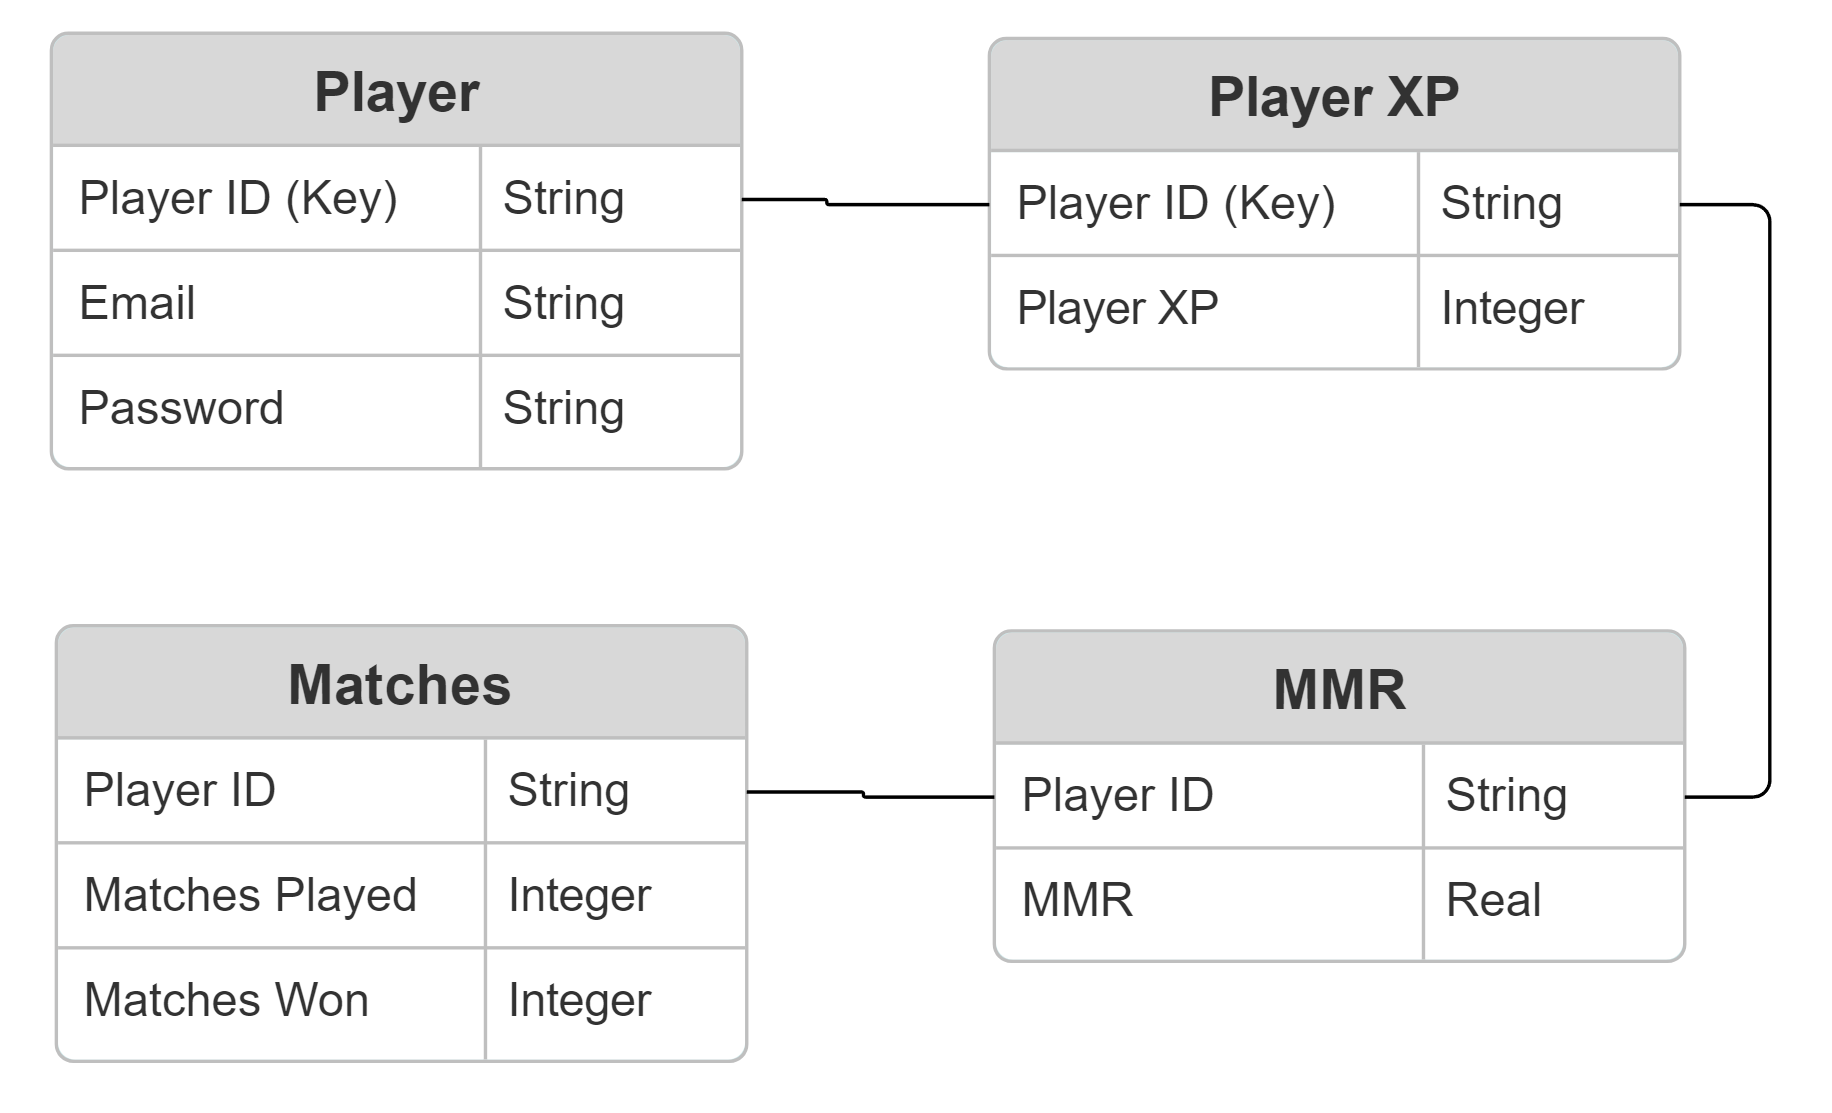
\includegraphics[width=15cm]{Design/Images/Database_Structure.png}
    \caption{An ER diagram of the database structure}
    \label{fig:db_structure}
\end{figure}

\vs
This database structure is justified because it is in 3NF. This means that we can query and search the database effectively and maintain referential integrity across the tables. We have chosen Player ID to be a key across the entire database because this will allow us to access all user information given the ID of the player. They will also be using this to login, and so we can quickly verify their login credentials when they are trying to login.

\tbc

\subsection{\textcolor{red}{UI}}

UI is essential to ensure that a user is able to quickly understand what each button does, and how to access what they need. For this reason, the only buttons present on the main menu will be "Play", "Settings", "Exit". This reduces any confusions that players may have, and allows the game to be much easier to pick up.

\vs
Here are some flowcharts detailing how the UI will lead to different sections of the game.


\vs

Additionally, we will now examine some different elements of the UI and justify why they are designed in a specific manner.

\vs
Firstly, I have chosen Iosevka as my font, as it is a sleek, modern font which I think is quite readable, but is very unique. This adds a unique element to the game.

\subsubsection{\textcolor{red}{Start Menu}}

The start menu will lead to the login menu, and so we really just want to provide a button for the player to click on. This is shown in Box INSERT FIGURE AND BOX NUMBER HERE.

The box will have a background colour which will be different to the rest of the screen in order to highlight that they can click there. This is important because usually in applications the cursor changes if you can click on something, however that is not the case here, and so we need to provide another way of conveying that information.

\vs
\subsubsection{\textcolor{red}{Login Menu}}

\vs
In the login menu, we want to allow the user to enter in their details and click submit to authenticate their account. This will be linked to the database handler, and so will need to provide the password to the database handler.



\subsubsection{\textcolor{red}{Main Menu}}

The main menu will house all of the other options that are available to the user, and so as shown in INSERT FIGURE AND DIAGRAM HERE, I have placed buttons adjacent to each other in a way that is intuitive.

\vs
Additionally, as seen in Box (INSERT BOX LETTERS HERE), we can see that there is still a background behind each box as explained previously.

\vs
Additionally, as shown in Box (INSERT LETTERS HERE), we can see the game's logo to create a sense of excitement, and since this is fairly common for games to do.

\subsubsection{\textcolor{red}{Set Timer}}

Here, we want to set the global timer, which will shut the game off after a game is finished. This will mean that we need to set a definite time limit as dictated by the user. We will also display the time at which the user's time will be over, so that they are aware of how long they have left.

INSERT DIAGRAM HERE

\subsubsection{\textcolor{red}{Create Game}}

In this menu, we want to be able to set the game's difficulty. This is done using arrows, since this seems to be the most intuitive way of doing something like this. Alternatively, a plus sign and a minus sign could be used also, since those explain more clearly what is going on.

INSERT DIAGRAM HERE

\subsubsection{\textcolor{red}{Game Loop}}

In the main game loop, we still have some UI elements to draw on. Primarily, we need to draw on the time as shown in Box INSERT BOXHERE, and we can draw other elements in a more clear way, such as by writing the amount of health each player has on the player itself, which quite clearly shows what is going on.

\vs

INSERT DIAGRAM HERE


\subsubsection{\textcolor{red}{Game Over}}

Once the game is over, we want to show the player where they have ranked relative to the other players.

INSERT DIAGRAM HERE

\subsubsection{\textcolor{red}{Leader Board}}


INSERT DIAGRAM HERE

\tbc

\subsection{\textcolor{red}{AI}}

I will be using PyTorch in order to handle the reinforcement learning aspect of the project. This is because it has extensive reinforcement learning tools, and is something which I am familiar with. Reinforcement learning works by using neural networks to create an output given a set of inputs. This is then processed and the action is taken. A reward is then assigned to this new state, and based on this, the model is adjusted through back-propagation and another step is taken. This continues millions of times, and this allows for the model to become progressively better. In order to create a game-like scenario, there will be 8 bots in two teams which will play against each other. The inputs to the bots are as follows, and all of this information will be condensed into a vector which is fed into the model.

\vs
\begin{enumerate}[label=\arabic*)]
    \item Current ammo - Provided as a real value between 0 and 1, denoting the proportion of ammo left, and computed by dividing the current amount of ammo by the ammo in a full weapon
    \item Current Health - Provided as real value between 0 and 1, and is computed by dividing the current health by the total health
    \item Distance to nearest health pad - This is given as a real value, and will be calculated using $r = \sqrt{(x_0 - x_1)^2 + (y_0 - y_1)^2}$, for the bot at $(x_0, y_0)$, and a health pack at $(x_1, y_1)$.
    \item Angle to nearest health pad - This is given as a real value, and can be calculated by $\arctan \frac{y_1 - y_0}{x_1 - x_0}$
    \item Spokes protruding from the centre of the players will extend to a set distance $r$, and will return 0 if there is no objects obstructing the spoke, will return $d$ if there is any enemy at distance $d$ from the centre of the player along that spoke, where $d<r$, and $-d$ if there is a wall obstructing the spoke at a distance $d<r$.
\end{enumerate}

\vs
The best model for this project is multi-agent reinforcement learning, as this will allow me to generate multiple bots which can compete against each other. Something like Deep Q Networks would not function in this environment because of the continuous nature of the game and the complex nature of the game.

\vs
The algorithm we will be using is Proximal Policy Optimisation, which relies on a clipped surrogate objective. This is an algorithm which can be expanded to a multi-agent version, which is what we want.

\vs
In order to do this, there will be a shared experience buffer, which will allow the agents to learn much faster than if they were playing individually. In order to allow the player to play, during the actual game, one of the agents will be "turned off", restricting the inputs that the AI gives, but still allowing the data buffer from the player to be transferred to the other two bots. This gives the game the feeling of playing with a team, rather than a more individual experience. This variant of the original Proximal Policy Optimisation which we will be using specifically, is known as MAPPO (Multi-agent Proximal Policy Optimisation) which uses centralised training, and decentralised execution. This is perfect for our situation, because, the player will not be able to communicate with the other bots during the game, and so it is ideal to have to have decentralised training and critics.

\vs
Additionally, during training, the rendering can be disabled, and the frame rate set to a very high value, in order to increase the speed at which the models can be trained. Because the model will progress from one frame to the next, the speed between frames can be altered without any consequence on the other bots on the team.

\vs
Furthermore, we will use a technique known as self-play. This is relevant since this is a competitive / co-operative game, we will put two separate versions of the model against each other. This will allow the model to play against "players" of it's own strength, and will produce better training results. Additionally, we don't have any ready-made players to play against, so this is our only option. We will initialise the model with random values to begin with, and will train it against itself in the first iteration. 

\vs
After this, we will take a snapshot of both agents, and then we will stop training the second agent, but keep updating the first one. With this, we can then train for a few more episodes and then take another snapshot of the agent. We will then sample the most recent models from the snapshot window and then train our agent against those. This will provide a way to train the AI against a wide variety of different agents which may have different ways of playing the game.

\vs
The first thing we need to in order to train the AI is to create an environment in order to train it. We will be using the \m{PettingZoo} wrapper to do this. This provides a strictly defined way of stating the game, using observation spaces, action spaces and rewards.

\vs
The observation space is the things which each agent can see. In the design section, we mentioned that each agent will have spokes which go out from the centre of the player. This will let the agents see the environment around them in a limited way.

\vs
The action space is all of the possible actions that the agent can take from any one state. The model will predict what it thinks is the optimal move to take from a given state depending on the observations that each agent can see.

\vs
The actions are then fed into the environment, and this is then used to move to the next time-step of the environment. With this, we can then return rewards, which are used to update the actor and critic networks. The reward is based on the actions of the player. For example, if the agent is able to eliminate another player, then this will result in a positive reward, but if the agent is shot, this will result in a negative reward.

\vs
The algorithm we will be implementing is known as MAPPO, which is the multi-agent variant of Proximal Policy Optimisation, which aims to optimise a surrogate objective function, but clips the maximum change that each time step can make to the actor and policy networks. This is in order to prevent large policy changes which could potentially damage the performance of the agent significantly. There are two networks used, the actor network, and the critic network.

\vs
Both networks use the same input, which is the observation for that time-step to generate an output. The actor outputs a vector which is the action which the agent will take in the following time-step. The critic network will output a single value, which is the predicted value of the state (or in other words, what it thinks the reward is going to be in that state).

\vs
From the original paper, we can see the process unfolding as follows. We firstly initialise our networks, and start a loop, and we can train for as long as we like. We then execute something known as a policy roll-out. This is effectively running our agent in the environment for a few time-steps, and recording the observations, actions, rewards and resulting states. This will allow us to gather information to train our network with. We also compute something known as advantages. Effectively, this gives us an idea of how much better off we are due to an action. We use a discount parameter and a GAE parameter.

\vs
On top of this, we will be using a library called \m{TianShou} which provides a high-level API on top of PyTorch in order to implement reinforcement learning algorithms. Additionally, it supports multi-agent reinforcement learning with heterogenous agents (agents which are not the same), and will allow us to do self-play to train the agents.

\vs


\subsection{\textcolor{red}{Utility Class}}

There are a lot of maths related functions which we will need to use particularly in detecting collisions with players, objects and rays. In particular we will need the following to be implemented.

\vs
We will first look at line-to-line collisions, since they underpin a large proportion of the game. Once, we can do line-to-line collisions we can also do line-to-rectangle collisions which are important for the weapon aspect of the game. We can derive a formula for how far along the ray the collision occurs. In the entirety of the game, we want to work with vectors and scales of 0 to 1 between the start and endpoints. Let us call these constrains $\vec{p_1}$ and $\vec{p_2}$ for line 1, and $\vec{p_3}$ and $\vec{p_4}$ for line 2. We first find a possible solution, then check that it the values that we have received are both between 0 and 1, since they are both bound segments.

\vs

\begin{align*}
	\vec{d_1} &= \vec{p_2} - \vec{p_1}\\
	\vec{d_2} &= \vec{p_4} - \vec{p_3}\\
	\text{Line 1: } \vec{r_1} &= \vec{p_1} + \lambda \vec{d_1}\\
	\text{Line 2: } \vec{r_2} &= \vec{p_3} + \mu \vec{d_2}\\
	\vec{p_1} + \lambda \vec{d_1} &= \vec{p_3} + \mu \vec{d_2}\\
	\vec{p_1} + \lambda(\vec{p_2} - \vec{p_1}) &= \vec{p_3} + \mu (\vec{p_4} - \vec{p_3})\\
	\begin{bmatrix} \lambda x_2 + (1 - \lambda)x_1 \\ \lambda y_2 + (1 - \lambda) y_1 \end{bmatrix} &= \begin{bmatrix} \mu x_4 + (1 - \mu)x_3 \\ \mu y_4 + (1 - \mu) y_3 \end{bmatrix}\\
	x_1 + \lambda (x_2 - x_1) &= x_3 + \mu (x_4 - x_3)\\
	y_1 + \lambda (y_2 - y_1) &= y_3 + \mu (y_4 - y_3)\\
	\lambda (x_2 - x_1) + \mu (x_3 - x_4) &= x_3 - x_1\\
	\lambda (y_2 - y_1) + \mu (y_3 - y_4) &= y_3 - y_1\\
    \begin{bmatrix} x_2 - x_1 & x_3 - x_4 \\ y_2 - y_1 & y_3 - y_4 \end{bmatrix} \begin{bmatrix} \lambda \\ \mu \end{bmatrix} &= \begin{bmatrix} y_2 - y_1 \\ y_3 - y_4 \end{bmatrix}\\
\end{align*}

\vs
We have arrived at a series of simulataneous equations. These can be easily solved with the \m{np.linalg.solve()} in NumPy, which means we don't have to solve it ourselves. However, this does have one restriction that the equations must be linearly indepenent. This just means that we need to check before hand what the determinant of the matrix is.
\vs

We also need to implement some more methods that are really important to the game and are going to be used repeatedly. These are addition, subtraction and the dot product. These are the most frequently used in vector equations and so are important to have implemented. This also gives us a quick way of finding the square of the magnitude of a vector by taking a dot product with itself.

\vs
In order to add or subtract two vectors, we can just take each element of the vector and add or subtract these elements to get our final result. Since all of our vectors are only having two dimensions we can just do this manually, or using list comprehension which is much more readable and easier to debug.

\vs
Furthermore, we need to have methods for collisions which we will be doing repeatedly throughout the game, and so this is best abstracted into the \m{Utility} class such that we can worry about other implementation details instead of re-coding the same methods over and over again.

\vs
In order to do this, we can split the collisions into a few main components. The first one is between two players. Since the players are rendered as circles, we can use this to find how to adjust the player positions.

\vs
Here is a diagram INSERT DIAGRAM HERE, showing two players overlapping. We can immediately see a few important details. The first one is that the distance between the two player's centres must be shorter than 2 times the radius of the player, since this will mean that the players are overlapping.

\vs
In order to resolve the collision, we need to move a player by an amount such that they will no longer be colliding, but just touching. Assuming that there is a collision, the derivation for the amount to the move the player by is as follows.

\begin{align*}
    TODO &= NOT+DONE+YET\\
\end{align*}

\vs
On top of this we need some way to handle collisions between lines and circles. This is because one of our primary success criteria was that there had to be weapons in the game, and that the user had to be able to shoot other players and that damage had to be processed.

\vs
During my research I found this method to detect a collision between a line and circle is two constraint points were used. This method involved computing multiple dot products until a quadratic equation was reached, and from there, it was just a simple comparision to find whether a collision had occurred.


\vs
Furthermore, since there will be blocks in the game, the player must not be able to pass through them and neither should any fired rays. In order to satisfy this, we need to consider two more types of collisions.

\vs
The first type is between a line and rectangle. This is quite simple, since we can just break a rectangle down into 4 lines and check for intersections with each one. We just want to find the intersection which is closest to the origin of the ray.

\vs
The second type of collision is between a circle and a rectangle. In order to do this, we need to find the point on the rectangle which is closest to the rectangle. In order to do this, I have referred to \cite{rectangle_circle_collision}, which explains in detail how this is handled.

\vs
This will then let us resolve the collision by moving it an appropriate distance.

\vs
Now that we have looked at how this works in theory, we should discuss how this works in implementation. In order to speed up the process as much as possible, I have considered other libraries to handle mathematical operations, such as adding vectors, dot products, matrices, etc.

\vs
The most popular scientific computing library in Python is \m{NumPy}, which provides a lot of different methods all written in native C code, and compiled providing extremely fast computations. However, there is one issue with this, in that in order to use \m{NumPy} methods we need to be working with NumPy objects. This is an issue because creating NumPy objects like arrays is incredibly slow, and therefore we will need to assess whether it is worth using this at all, since it is very plausible that casting to NumPy objects is slow enough to outweight the efficiency of using NumPy methods.


\clearpage
\section{Development - Iteration 1}
\subsection{Main}

To begin this iteration, we will start by implementing the base of the game. To start with, we will import PyGame, and define the display size and mode and tick rate. This is in \m{main.py}.
\vs

\begin{mpy}
#PyGame modules
import pygame
from pygame.locals import *
import sys
\end{mpy}

\vs
We will be running the game at 240 frames per second, which will be a lot higher than what most people will really be able to run the game at, but there is a good reason for this. With this high frame rate, we will get smooth gameplay regardless of the monitor's frame rate. This justifies it because it provides a similar experience for everyone playing the game, and will mean that the computer's hardware is taken full advantage of. We will be using frame-rate independent physics in order to ensure a fair game regardless of a person's device. Additionally, when we are training the AI, we will be disabling rendering, since it serves no purpose to use a rendering tool. This will allow for a substantial increase in performance and allow for very quick training.
\vs
\subsection{Game State Manager}

\vs
Now, we will create a game state manager. This will handle which state the game is currently in, and which state it will move to next. We will also pass global information, like timers, display size, refresh rate, etc, to this game state manager so that the other states, menus and the game loop itself can access this information.

\vs
\begin{mpy}
class GameStateManager:
  def __init__(self, current_state, SCREEN_DIMS, REFRESH_RATE):

    #Get the global game variables in a convenient way
    #Allows all states to easily access these values
    self.current_state = current_state
    self.SCREEN_DIMS = SCREEN_DIMS
    self.REFRESH_RATE = REFRESH_RATE

  #Returns the current state of the game
  def getState(self):
    return self.current_state

  #Set the next state of the game (ie. game loop -> game over)
  def setState(self, state):
    self.current_state = state
\end{mpy}

\vs

We can try and set and get states from the \m{GameStateManager} as follows.

\vs
\begin{mpy}
>>> gsm = GameStateManager('start', SCREEN_DIMS, REFRESH_RATE)
>>> gsm.get_state()
start
>>> gsm.set_state('next_state')
>>> gsm.get_state()
next_state
\end{mpy}
\vs
We assign the game state manager's attributes as the inputs we have defined. There will only be one instance of the game state manager, and therefore, this is going to allow us to access the game state manager within every state. However, in order to do that, we need to pass the instance of the manager into each of the states.


\vs

\subsection{\textcolor{blue}{Player}}

We need to define a player class, a menu class and a weapon class. This will form the basis of our game.
\vs

\begin{mpy}
class Player(pygame.sprite.Sprite):

  def __init__(self, spawn_point, initial_forward_vec, team, weapon):

    #Initialise the PyGame sprite
    pygame.sprite.Sprite.__init__(self)

    #Where the player will spawn every time they are killed
    self.spawn_point = spawn_point

    #The direction the player will face when they are respawned
    self.initial_forward_vec = initial_forward_vec

    #The maximum health that the player can have at any time
    self.max_health = 100

    #The current health of the player
    self.health = 100

    #The maximum magnitude of the velocity
    self.max_speed = 300

    #Which team the player is on, it will be an integer (0 or 1)
    #To check for a hit between two enemies
    #XOR the teams of the two players involved (0 means no hit, 1 means hit)
    self.team = team

    #The player's Weapon
    self.weapon = weapon

    #Current position of the players
    self.position = self.spawn_point

    #Current direction of the player
    self.forward_vec = self.initial_forward_vec

    #Radius of the circle representing the player
    self.radius = 75
\end{mpy}
\vs
The first, most obvious thing to implement is a way to move the player. This must be done using the inputs from the keyboard. We will set a maximum velocity, and use the keyboard inputs to find this value. However, we will do this in the game loop. For now, we will be implementing a move function, which will let us move the player on the map depending on the input. This is helpful, because this input could come from a human player, or an AI.
\vs

\begin{mpy}
  def move_player(self, directions, dt):
    #velocity = [Forward, Right] components
    velocity = [0, 0]

    #For loop avoids repeated code
    for i in (0, 2):
      if directions[i] == directions[i+1]:
        velocity[i//2] = 0
      else:
        velocity[i//2] = directions[i] - directions[i+1]

    #Velocity will have -1, 0, or 1 in each spot
    #If it is moving diagonally, x^2 + y^2 = 2
    #So we must divide the components by sqrt(2)
    if (velocity[0]**2 + velocity[1]**2 == 2):
      velocity = [i / 2**(1/2) for i in velocity]

    #We need to multiply by the max speed in order to get our final velocity
    velocity = [self.max_speed * i for i in velocity]

    #We will finally update the position of the player
    self.position = [self.position[i] + velocity[i]*dt for i in (0, 1)]


\end{mpy}
\vs

We can test this code as shown below. 

\begin{mpy}
>>> p = Player([4000, 4000], [0, -1], None, None)
>>> p.move([0, 0, 0, 0], 1)
>>> p.position
[4000, 4000]
>>> p.move([1, 1, 0, 0], 1)
>>> p.position
[4000, 4000]
>>> p.move([1, 0, 1, 0], 1)
>>> p.position
[4353.553390593273, 4353.553390593273]
\end{mpy}

\vs
This is what we have expected and so this function works as expected. The input to the function will be sanitised in the game loop, so there is no way for a user to enter invalid inputs. However, there is one thing we need to do. Primarily, we need to find a way to limit the player's movement between 0 and 8000. This can be done as follows.

\begin{mpy}
    #Update position of player
    updated_position = [self.position[i] + velocity[i]*dt for i in (0, 1)]

    #Check that the values are within (0, 0) and (8000, 8000)
    #(0, 0) is the top left of the map
    #(8000, 8000) is the bottom right

    for i in range(2):
        
      if updated_position[i] - self.radius <= 0:
        updated_position[i] = self.radius

      elif updated_position[i] + self.radius >= 8000:
        updated_position[i] = 8000 - self.radius

    self.position = updated_position
\end{mpy}

\vs

As mentioned in the design section, we want to only render the area around the player, and hence, we will define a \m{CameraPosition}. This will let us draw only things which are on the screen relative to the player. We can calculate the relative position of the players relative to this camera position, since we will also be using bots in the game. However, if the \m{Player} instance is for the user, then, it will just return the centre of the screen, because we want to keep the player at the centre of the screen.
\vs
\begin{mpy}
  #Will convert the world position of the character to a camera position for the player
  def convertToScreen(self, camera_position, object_position, SCREEN_DIMS):
    screenPosition = [object_position[i] - camera_position[i] + SCREEN_DIMS[i]//2 for i in (0, 1)]
    return screenPosition

\end{mpy}
\vs
We will also write a rendering function, in order to remove this from the game loop, which is helpful because different objects will be rendered differently, but letting all of them have their own render functions, will let us loop through all of the objects on the map and render them effectively.
\vs
\begin{mpy}
  #Renders the character to the display of the player
  def render(self, display, camera_position, directions, dt, SCREEN_DIMS):
    #Add code to not render if outside frame
    pygame.draw.circle(display, self.colour, self.convertToScreen(camera_position, self.position, SCREEN_DIMS), self.radius)
    for_pos = [self.position[i] + 100*self.forward_vec[i] for i in range(2)]
    pygame.draw.aaline(display, (100, 0, 0), self.convertToScreen(camera_position, self.position, SCREEN_DIMS), self.convertToScreen(camera_position, for_pos, SCREEN_DIMS))
    self.move_player(directions, self.forward_vec, dt)
\end{mpy}

The player is rendered as just a circle for now, maybe later to be replaced with something else. The \m{pygame.draw} methods are from the documentation, and we convert the position to the screen position so that the player remains stationary relative to the screen and everything else moves relative to them. This will ensure a more intuitive game experience.

\subsection{\textcolor{blue}{Database Handling}}

We will be using SQLite 3, since the project is small and likely to have only a few users. We are also not editing extremely frequently, only to create users, to login / register, or to update accounts after a game. Therefore, we can create a class to handle the management of the database, which we will call \m{DatabaseHandler}. We will define \m{SetupConnection()}, which will let the class instance connect to the database, and \m{CloseConnection()}, which will safely close the connection. This will ensure that we don't have issues in committing our changes to the database, and will ensure data safety.

\vs
\begin{mpy}
class DatabaseHandler:

  #Setup a cursor and connection in order to allow for queries and updates
  def SetupConnection(self):
    self.connection = sqlite3.connect("momentum_users.db")
    self.cursor = self.connection.cursor()

  #Close connection to prevent database corruption or multiple write attempts
  def CloseConnection(self):
    self.connection.close()
\end{mpy}
\vs
We will also define two more methods on our class, which are \m{CreateAccount()}, and \m{UpdateAccount()}, which are pretty self-explanatory. We want to be able to maintain referential integrity and atomicity, so for that reason only commit once all of the instructions that need to be commited have been passed to the cursor. This is important because it means that if there is an issue in one of the statements, then we don't break referential integrity across the database. There is no way to really check that these commands work, so we will just have to use them in the next commands ensure that they work there. There are no inputs from this, so we can't really "break" these functions anyway.

\vs
\begin{mpy}
  def CreateAccount(self, PlayerID, Email, Password):
    #Setup connection and cursor
    self.SetupConnection()

    #Insert data into each of the tables individually
    self.cursor.execute(f"INSERT INTO Player VALUES('{PlayerID}', '{Email}', '{Password}')")
    self.cursor.execute(f"INSERT INTO PlayerXP VALUES('{PlayerID}', 0)")
    self.cursor.execute(f"INSERT INTO MMR VALUES('{PlayerID}', 1000)")
    self.cursor.execute(f"INSERT INTO Matches VALUES('{PlayerID}', 0, 0)")

    #Commit and close connection
    self.connection.commit()
    self.CloseConnection()

  def UpdateAccount(self, PlayerID, PlayerXP, MMR, MatchWon):
    #Setup connection and cursor
    self.SetupConnection()

    #Update each statistic
    self.cursor.execute(f"UPDATE PlayerXP SET PlayerXP = PlayerXP + {PlayerXP} WHERE PlayerID = '{PlayerID}'")
    self.cursor.execute(f"UPDATE MMR SET MMR = {MMR} WHERE PlayerID = '{PlayerID}'")
    self.cursor.execute(f"UPDATE Matches SET MatchesPlayed = MatchesPlayed + 1, MatchesWon = MatchesWon + {MatchWon} WHERE PlayerID = '{PlayerID}'")

    #Commit and close connection
    self.connection.commit()
    self.CloseConnection()

\end{mpy}
\vs
In the \m{UpdateAccount()} method, we have simply taken the change in PlayerXP and whether the Match was won or not. This is helpful because it reduces the number of calls we need to make. This is because, we know that if we are calling this method, we have just completed another game, and so the number of matches played must increase by one, and whether the match was won or not is simply just a one or a zero. This means we don't need to find this information from the database using a query before inserting it back. This also reduces the chance of some error happening during this transition, and reduces the time taken.
\vs

We will now test these functions to make sure that they work and that we can succesfully link to the database. To ensure that this happens, we first need to create a database. This will follow the specification laid out in the design section. We will be using SQLite3 here, since it is a lightweight framework to use instead of a more concrete SQL package which would take a significant amount of work to setup.

\vs
We can test it as follows. We will use the functions to create and update an account, and then use another function to get this data back. We will now construct the function to get the user information. This will also be useful when constructing the leaderboard. We will first use \m{fstring} in order to format the strings in a concise and quick manner. This is shown as below.

\vs
\begin{mpy}
>>> PlayerID = "Ojas"
>>> f"SELECT * WHERE PlayerID = '{PlayerID}'"
"SELECT * WHERE PlayerID = 'Ojas'"
\end{mpy}

\vs
This is used as follows. For now, this will just return the data from one table, but we can expand it to give back the data from all of our tables. We can return the information as a dictionary which will make the data more processable and easier to work with.

\vs
\begin{mpy}
  def fetchUserInfo(self, PlayerID):
    self.SetupConnection()

    userInfo = {'PlayerID': PlayerID}

    result = self.cursor.execute(f"SELECT * FROM Player WHERE PlayerID = '{PlayerID}'")

    userInfo['email'] = result[1]
    userInfo['password'] = result[2]

    return userInfo
\end{mpy}

We will now insert the following data into our database using the \m{CreateAccount()} method. We will then use the method above to get more data back.

\begin{mpy}
>>> dbh = DatabaseHandler()
>>> DatabaseHandler.CreateAccount("ojas_tiwari", "tiwariojas@gmail.com", "HelloAgain")
>>> dbh.fetchUserInfo("ojas_tiwari")
{'PlayerID': 'ojas_tiwari', 'email': 'tiwariojas@gmail.com', 'password': 'HelloAgain'}
\end{mpy}

This proves that our connection works, and that we can create accounts and fetch some user information. We will add to the \m{fetchUserInfo()} method when we need more information on the player.
\vs


Finally, we also need to define an authentication query, which will return true or false, depending on whether the user has inputted the correct credentials for their account. We will return a list, with one element if they have submitted the correct credentials, simplying containing \m{[True]}. Otherwise, they will get an array with two elements, the first containing \m{False}, and the second element will be the reason for their query being rejected either \m{'invalid_id'} or \m{'invalid_password'}. These are fairly self-explanatory, and will be used to show the user why the could not login.
\vs
\begin{mpy}
  def AuthenticateAccount(self, PlayerID, Password):
    #Setup connection and cursor
    self.SetupConnection()

    #Query player database
    result = self.cursor.execute(f"SELECT Password FROM Player WHERE PlayerID = '{PlayerID}'").fetchone()

    #Nothing to commit here, just close
    self.CloseConnection()

    #Use of a guard clause instead of a double conditional
    if result == None:
      return [False, 'invalid_id']
    if Password == result[0]:
      return [True]
    return [False, 'invalid_password']
\end{mpy}
\vs
We have used a guard clause in order to decrease the amount of code written.

\subsection{\textcolor{blue}{Utilities}}

We need to be able to do many vector operations quickly without having to re-write the code consistently. This also allows us to more easily test all of these methods and ensure that they are working properly. We need to be certain that they are accurate and are providing reproducible results. To that extent, we will define a new class \m{Utility} which will handle all of these calls. A lot of these vector calculations are quite complicated so to that end they have been referenced from other resources and have been listed in this document. I have put this towards the start of the development section since, lots of other things rely on this, and it was essential to getting the rest of the code to work.

\vs
We begin by defining our class.
\begin{mpy}
class Utility:

  def __init__(self):
    #Nothing to do here so far
    pass

  def dot(self, a, b):
    return sum([i*j for i, j in zip(a, b)])
\end{mpy}

\vs
The first method we have implemented is the dot product. For geometric vectors this is defined as 
\begin{align*}
  \vec{a} \cdot \vec{b} &= \sum_i a_i b_i\\
\end{align*}
Where $a_i$ refers to the $i$-th element of $\vec{a}$. Then, in Python, we can use the \m{zip()} function in order to get a list of tuples of corresponding elements, as shown below.
\begin{mpy}
for i in zip([1, 2, 3], [4, 5, 6]):
  print(i)

>>> (1, 4)
  (2, 5)
  (3, 6)
\end{mpy}

\vs
Then, we want to multiply the numbers in each pair together. We can directly access the elements using $i, j$ instead of just $i$ in the for loop, and thus we can instantly multiply them. We then create a list of these which produces this output.

\begin{mpy}
dottedVals = []
for i, j in zip([1, 2, 3], [4, 5, 6])
  dottedVals.append(i * j)
print(dottedVals)

>>> [4, 10, 18]
\end{mpy}

\vs
Finally, we need to take the sum of all of these, which we can do using \m{sum()}. This finally gives us the following.

\begin{mpy}
sum(dottedValues)

>>> 32
\end{mpy}
However, we can condense this code slightly, by using list comprehension. We can rewrite \m{dottedVals} as follows, and can then just remove it all together.

\vs
\begin{mpy}
dotProdut = sum([i * j for i, j in zip(a, b)])
\end{mpy}

\vs
We can test this out using two dummy arrays. I also don't want to create instances of the \m{Utility} class as this will occupy even more memory.

\begin{mpy}
>>> a, b = [1, 2, 3], [4, 5, 6]
>>> Utility.dot(a, b)
TypeError: Utility.dot() missing 1 required positional argument: 'b'
\end{mpy}
\vs

In order to solve this, there are two approaches. Firstly, we could just create an instance of the \m{Utility} class, and then call the function. However, we do not want to do this because this would occupy a lot more memory.

\vs
The other alternative is to use the \m{@staticmethod} decorator and to remove \m{self} parameter from the function definition. The code then works as expected.

\begin{mpy}
>>> Utility.dot([1, 2, 3], [4, 5, 6])

32
\end{mpy}
Finally, I also considered using the library \m{NumPy} to do the dot product as it is already implemented. To decide which one to use, I decided to test it out by looking at how long it took to dot product lots of arrays. Since all of my vectors are 2D, they will only have 2 elements, and so that is what I used here.

\vs
\begin{mpy}
import numpy as np
import time
import random

time1 = time.time()

for i in range(10000):
  a = [random.random() for i in range(2)]
  b = [random.random() for i in range(2)]
  x = int(np.dot(a, b))
  
print("NumPy:", time.time()-time1)


class Utility:
  @staticmethod
  def dot(a, b):
    return sum([i*j for i, j in zip(a, b)])
    
time3 = time.time()

for i in range(10000):
  a = [random.random() for i in range(2)]
  b = [random.random() for i in range(2)]
  y = Utility.dot(a, b)
  
print("Raw Python:", (time.time() - time3))
\end{mpy}
\vs
Looking at the results, we see that the raw Python implementation is much faster than the \m{NumPy} implementation. This is likely due to the fact that \m{NumPy} needs to convert lists into \m{NumPy} arrays in order to be able to compute the dot product.

\begin{mpy}
NumPy: 0.3286013603210449
Raw Python: 0.17571258544921875
\end{mpy}
\vs
Therefore, I will use the Python implementation.

\vs
Additionally, we will construct addition and subtraction for vectors. Another possible consideration was to just use NumPy throughout the game, and I don't know why I didn't do this.... 

\begin{mpy}
  @staticmethod
  def vecSub(a, b):
    return [i-j for i, j in zip(a, b)]

  @staticmethod
  def vecAdd(a, b):
    return [i + j for i, j in zip(a, b)]
\end{mpy}
\vs

We can test these out as shown below.
\vs

\begin{mpy}
>>> Utility.vecSub([4, 5, 6], [1, 2, 3])
[3, 3, 3]
>>> Utility.vecAdd([1, 2, 3], [4, 5, 6])
[5, 7, 9]
\end{mpy}

\vs
Next, we will need to implement a collision between a ray and a circle. This is important as this will be used to detect when a weapon has fired a ray that has hit another player. We will be using the implementation from \href{https://codereview.stackexchange.com/questions/86421/line-segment-to-circle-collision-algorithm}{this StackExchange post}, which uses vectors in order to solve this problem. This is much more efficient than using Cartesian co-ordinates.

\vs
\begin{mpy}
  @staticmethod
  def lineCircleCollision(line, circle):
  
    #Notation from the StackExchange post
    q = circle[0]
    r = circle[1]
    p1 = line[0]
    v = Utility.vecSub(line[1], p1)

    a = Utility.dot(v, v)
    b = 2 * Utility.dot(v, Utility.vecSub(p1, q))
    c = Utility.dot(p1, p1) + Utility.dot(q, q) - 2 * Utility.dot(p1, q) - r**2

    discriminant = b**2 - 4 * a * c

    if discriminant < 0:
      return [False, None]

    sqrt_disc = sqrt(discriminant)
    
    t1 = (-b + sqrt_disc) / (2 * a)
    t2 = (-b - sqrt_disc) / (2 * a)

    if not (0 <= t1 <= 1 or 0 <= t2 <= 1):
      return [False, None]
    
    t = min(t1, t2)
    return [True, t]
\end{mpy}

\vs
In this implementation, we do not provide a direction vector, rather we provide two constraint points. This solution is much more optimal, since it means we do not also need to provide a range parameter. We simply want to find the closest collision to the source, and this will provide it if a collision is found. The $t$-value must be between $0$ and $1$ where $0$ would mean that the source is right next to the circle we are checking for a collision with, and $1$ means that the second constraint point lies on the circle. We can test this code out as follows.

\vs

We will first check the two standard cases; one where the collision does occur and one where it doesn't.

\begin{mpy}
>>> line = [[0, 0], [10, 5]]
>>> circle = [[2, 3], 2]
>>> Utility.lineCircleCollision(line, circle)
[True, 0.2]
\end{mpy}

\vs
We can check manually, or using plotting software that this does indeed work. We will now check when there should not be a collision.

\vs
\begin{mpy}
>>> line = [[2, 3], [-5, -6]]
>>> circle = [[5, 10] , 2]
>>> Utility.lineCircleCollision(line, circle)
[False, None]
\end{mpy}
\vs
This is as expected. Next, we will test when the second constraint is just on the circle.

\vs
\begin{mpy}
>>> line = [[0, 0], [5, 0]]
>>> circle = [[6, 0], 1]
>>> Utility.lineCircleCollision(line, circle)
[True, 1.0]
\end{mpy}
Again, this is the result we expected.

\vs
We will test the case where the first constraint is inside of the object, but not the second.
\begin{mpy}
>>> line = [[0, 0], [5, 10]]
>>> circle = [[2, 0], 2]
>>> Utility.lineCircleCollision(line, circle)
[True, 0.0]
\end{mpy}
\vs
Finally, despite this case never arising in an actual game, we will test the case where both constraints are inside of the circle.
\begin{mpy}
>>> line = [[0, 0], [0, 1]]
>>> circle = [[0, 0], 3]
>>> Utility.lineCircleCollision(line, circle)
[False, None]
\end{mpy}
Again, the desired result! So, we can conclude that the function works as expected.
%https://www.jeffreythompson.org/collision-detection/line-rect.php

\vs
We will now implement the line-line collision method we which described thoroughly in the design section. We will be using NumPy to do the solving of the simultaneous equations. We first need to check that the equations are linearly independent. We can do this using the determinant of the matrix. We will first be extracting all of the elements we need to make the rest of the code easier to read.

\begin{mpy}
  @staticmethod
    def lineLineCollision(line1, line2):
      #We have both lines in vector form
      #line 1 -> [x_1, y_1], [x_2, y_2]
      #line 2 -> [x_3, y_3], [x_4, y_4]
      x_1, y_1 = line1[0]
      x_2, y_2 = line1[1]
      x_3, y_3 = line2[0]
      x_4, y_4 = line2[1]
\end{mpy}

After this we can compute the determinant and if it is not 0, we can find the solutions.
\begin{mpy}
    #Find the determinant
    determinant = np.linalg.det(matrix)
    if determinant == 0:
      return [False, None]
          
    else:
      result = np.linalg.solve(matrix, resultVec)
          
      #Check that the result is between the constraint points
      if 0 <= result[0] <= 1 and 0 <= result[1] <= 1:
        return [True, result]
      return [False, None]
\end{mpy}

We can also edit this code to make it more readable by using a guard clause. Since we are returning if the determinant is 0, no other code after it will return if this condition is meant. Therefore, we can see that we don't need the \m{else} statement at all, and can instead dedent the code block there.

\begin{mpy}
    #det = 0 -> Can't be solved
    if determinant == 0:
      return [False, None]

    #Solve system
    result = np.linalg.solve(matrix, resultVec)

    #Check that the result is between the constraint points
    if 0 <= result[0] <= 1 and 0 <= result[1] <= 1:
      return [True, result]
    
    #Solution is not in bounds
    return [False, None]
\end{mpy}

\vs
We also want to be able to test this code and make sure that is efficient, since we are casting to a NumPy array this likely to not be very efficient. We are primarily interested in how iterations we can do in one second, since this will be very helpful during the training, and we want to make sure that the environment is easy to sample with.

\begin{mpy}
start = time.time()
for i in range(70000):
  line1 = [[random.uniform(0, 8000), random.uniform(0, 8000)], [random.uniform(0, 8000), random.uniform(0, 8000)]]
  line2 = [[random.uniform(0, 8000), random.uniform(0, 8000)], [random.uniform(0, 8000), random.uniform(0, 8000)]]
  x = Utility.lineLineCollision(line1, line2)
end = time.time()
print(end - start)

>>> 1.0048434734344482
\end{mpy}

This quite significant which means that we can do a lot of timesteps in one second, which will increase our overall training speed.

\vs

The next thing we will be implementing is the line-rectangle collision. We can decompose each rectangle into 4 lines between adjacent corners. Therefore, we need to create a method to get the corners of a rectangle. Therefore, we will create a new method in the \m{Block} class to get the corners.

\vs
\begin{mpy}
  def getCorners(self):
    #TL, BL, BR, TR
    corners = []

    for i in range(-1, 2, 2):
      for j in range(-1, 2, 2):
        corners.append(U.vecAdd(self.centre, [i * self.length1/2, i * j * self.length2/2]))

    return corners
\end{mpy}

\vs
The code is a bit dense, but we can prove that this code will work and then test it. We want to get the corners in an anti-clockwise order because this will give us the lines that we since the lines must be on the edges of the rectangle. We firstly create an array to store the co-ordinates of the corners in. Next, we create two for loops. The outer loop will take two values only, $-1$ and $+1$. This will show the direction of the horizontal movement from the centre. In the inner loop, we can either move upwards by half of the height of the rectangle, or we can move down by the same amount. This produces all 4 corners. If we just print $i$ and $ij$, we can see that the output is as follows.

\begin{mpy}
>>> for i in range(-1, 2, 2):
  for j in range(-1, 2, 2):
    print(i, i*j)

-1 1
-1 -1
1 -1
1 1
\end{mpy}
\vs

This can be plotted on the $x$ and $y$ axes, which is going anti-clockwise, and we are only changing one element of the co-ordinate at a time which means that we will only be putting adjacent vertices next to each other.

\vs
We can now test the code with some sample values.

\begin{mpy}
b = Block([1, 2], 10, 20, 'red', [1600, 900], [800, 450])
corners = b.getCorners()
print(corners)

>>> [[-4.0, 12.0], [-4.0, -8.0], [6.0, -8.0], [6.0, 12.0]]
\end{mpy}

This is what we would have expected to see. Now, that we have this, we want to find the edges of the rectangle. With this, we can generate the edges present.

\vs
\begin{mpy}
  @staticmethod
  def lineRectCollision(line, block):

    #Get the corners
    corners = block.getCorners()
    
    #Decompose the rectangle into 4 lines: TL -> TR, TR -> BR, BR -> BL, BL -> TL
    lines = [[corners[i], corners[i+1]] for i in range(-1, 3) ]
\end{mpy}

\vs
The second line is list comprehension which gives pairs of corners, and since we have arranged them to be adjacent to each other, the lines formed are all on the boundary of the rectangle. We only need the pairs of constraint points since that is what we are using for the line collision method.

\vs
The next thing we need, is to find the collision which is the closest to the first constraint point which is what our program returns.
\vs

\begin{mpy}
    #We only care about how far along the main line the collision is
    t_val = 3
    for edge in lines:
      isHit, lambda_mu = Utility.lineLineCollision(line, edge)
      if isHit:
        if lambda_mu[0] < t_val:
          t_val = lambda_mu[0]
\end{mpy}

\vs
We set \m{t_val} to be $3$ since the result of the collision must be between 0 and 1, and so this will be well outside of the range anyway. This also means that we can check if we ever updated the minimum collision distance.

\vs
\begin{mpy}
    if t_val == 3:
      return [False, None]
    return [True, t_val]
\end{mpy}

\vs
We can also return whether we have detected a collision or not, and if we have, then what that distance is. We will be testing a boundary case, where the line clips one of the edges of a rectangle, but should still return a hit.

\begin{mpy}
b = Block([0, 0], 10, 20, 'red', [1600, 900], [800, 450])
line = [[0, 20], [10, 0]]
result = U.lineRectCollision(line, b)
print(result)

>>> [True, 0.5]
\end{mpy}

\vs
We also need to define the method for converting a world position to a screen position which will let us actually render things, since the player's viewpoint moves as the player moves. We can do this as detailed in the Design section.

\begin{mpy}
  #Will convert the world position of the character to a camera position for the player
  @staticmethod
  def convertToScreen(camera_position, object_position, SCREEN_DIMS):
    screenPosition = [object_position[i] - camera_position[i] + SCREEN_DIMS[i]//2 for i in (0, 1)]
    return screenPosition
\end{mpy}

\vs
We have used list comprehension to compress our statements, since this is more efficient than using a for loop (from \cite{listcomp}), since they do not have an overhead in producing a for loop, and therefore, we have used this throughout the project. This means that we can now easily and efficiently call all of these functions and due to the stateless nature of the \m{Utility} class we don't need to worry about creating and deleting many instances, and this is also more efficient to do in Python, which has been a concern throughout the project, since we will be removing the render functions and will be using the game loop to do the training of the game. Therefore, every aspect of the game must be optimised to a reasonable extent in order to allow for more samples in a given period of time. As a result of this we will be removing the \m{convertToScreen} method from the \m{Player} class since it is no longer needed since we have already globalised its implementation to the \m{Utility} class.

Another method that we should implement since this is very commonly used is the scalar multiple of a vector. For this, we need two inputs, one is a vector and another is a scalar by which we need to multiply the vector by. This is done by list comprehension again.

\begin{mpy}
  @staticmethod
  def mult(vec, scalar):
    return [i * scalar for i in vec]
\end{mpy}

We simply take each element of the vector and then multiply it by the vector we took in. We can test it as follows.

\begin{mpy}
>>> Utility.mult([1, 2], 2)
[2, 4]
\end{mpy}

Additionally, we need to be able to rotate vectors, specifically to create spread in the weapon's fire, such as for the shotgun. We can do this as fllows. We consider the matrix ($\hat{A}$) for a 2D rotation which is written as follows.

\begin{align*}
  \hat{A}(\theta) &= \begin{bmatrix} \cos \theta & - \sin \theta \\ \sin \theta & \cos \theta \end{bmatrix}\\
\end{align*}

We can do a simple matrix-vector product as follows.
\begin{align*}
  \vec{r} &= \begin{bmatrix} x \\ y \end{bmatrix}\\
  \vec{r}' = \hat{A}\vec{r} &= \begin{bmatrix} x \cos \theta - y \sin \theta \\ x \sin \theta + y \cos \theta \end{bmatrix}\\
\end{align*}

This can then be converted into code as follows.

\begin{mpy}
  @staticmethod
  def rotateVector(vec, angle):
    #https://matthew-brett.github.io/teaching/rotation_2d.html
    rotatedVec = [0, 0]
    rotatedVec[0] = vec[0] * cos(angle) - vec[1] * sin(angle)
    rotatedVec[1] = vec[0] * sin(angle) + vec[1] * cos(angle)

    return rotatedVec
\end{mpy}

The \m{sin()} and \m{cos()} functions are from the \m{math} library which was imported at the start of the file. We can test this function as follows.

\begin{mpy}
>>> Utility.rotateVector([1, 0], math.pi/4)
[0.7071067811865476, 0.7071067811865476]
>>> 2**-0.5
0.7071067811865476
\end{mpy}

This means that we have rotated the vector anti-clockwise by an angle of \ang{45} or $\frac{pi}{4}$ radians. Furthermore, we can test this for other angles as well like \ang{90}.

\begin{mpy}
>>> Utility.rotateVector([1, 0], math.pi/2)
[6.123233995736766e-17, 1.0]
\end{mpy}

This is not exactly right, but it is close enough to what we need since we expected 1.0 in the $y$-ordinate, and the $x$-ordinate is so incredibly small that we would not be able to process such as a change anyway.


\subsection{\textcolor{blue}{Weapon}}
We will give each player a weapon, of a specific class, which will have specified statistics. In order to do this, we can create a parent class \m{Weapon} and derive other weapons from it. There are a few specific attributes that we need to have for the parent class. 
\vs
\begin{mpy}
class Weapon:
  #We need a way to move the weapon alongside the Weapon
  #Some way to attach the two together
  #TODO
  def __init__(self):
    self.ammo = 30
    self.reloadTime = 2.0
    self.damagePerHit = 5
    self.range = 1000
    self.std_dev = 0.25
    self.cooldown = 0.2
    self.raysPerShot = 1
    self.cooldown = 0.25
    self.spread = 1
\end{mpy}

We will now justify each attribute. The ammo is the largest amount of ammunition that the weapon can fire before needing to reload. This is important since otherwise a player could just hold down the fire button without needing to be aiming correctly. The reload time is the amount of time taken from emptying the weapon's "cartridge" to refilling it so that they player can fire the weapon again.

\vs
The damage per hit is self-explanatory, but every time a ray from that weapon hits a player, this is the amount of damage that is dealt. The range is the maximum distance that the ray can extend, and is used to find the end point of the ray that we will be using for the ray collision detection.

\vs
The standard deviation is used for the normal distribution to find how spread out the rays will be from the direction vector. We will be firing rays from the player, and then find an angle to rotate this vector by to find the ray's direction. We can do this as follows.

\begin{mpy}
>>> std_dev = 0.25
>>> np.random.normal(loc = 0, scale=std_dev, size=None)
0.3018635745361101
>>> np.random.normal(loc = 0, scale=std_dev, size=None)
-0.12774112426206038
>>> np.random.normal(loc=0, scale=0.25, size=None)
0.043154759156613466
\end{mpy}
\vs
This will let us create derived classes from this and then assign them each different values for these attributes. Alongside this, we can define a fire function, which will let us project a ray from the weapon's position and direction, and hand it over to the game loop to identify any collisions. Importantly, the ray is defined $\mathbf{r} + t \mathbf{d}$, where $\mathbf{r}$ is the position of the player, and $\mathbf{d}$ is the direction.
\vs

Therefore, our player will need to pass the position and direction from the \m{Player} class. This will then return a tuple of vectors which we then pass to the game loop.
\vs

We will take firing as being a Boolean, either 0 or 1. This will be whether we are currently firing the weapon or not, and will be taken from a mouse input. Furthermore, we will take the direction that the mouse is pointing in to be the direction of the player. $t$ must greater than 0, because this will allow us to trace the ray as it progress forward from the player, since it wouldn't make sense for it to move behind the player.
\vs

We also need to create attributes for the number of rays per shot as well as the angle of the rays as they spread out. For example, for a sniper, there is only ray produced and it doesn't deviate from the direction vector. To add this randomness, we can generate a random angle between 0 and the maximum limit according to a normal distribution or a uniform distribution, and then rotate the direction vector around each time. This will return an array of rays, which can then be passed on. Hence, for all fire functions, we will be returning an array which is iterated over. We also add a spread factor which is a boolean and will tell the \m{fire()} method whether to include a spread or not.
\vs


The rays will be randomly spread out. We can do this as follows.
\begin{mpy}
  #We will attach the damage to this as well
  def fire(self, position, direction):
    rays = []
    magnitude_squared = U.dot(direction, direction)
    unit_dir = U.mult(direction, 1 / sqrt(magnitude_squared))

    for i in range(self.raysPerShot):

      #Sample deviation using the normal distribution
      if self.spread == 1:
        angleDeviation = random.normal(loc = 0, scale=self.std_dev, size=None)
        rotated_dir = U.rotateVector(unit_dir, angleDeviation)
      else: 
        rotated_dir = unit_dir

      #Add unit_dir rotation here using matrices
      final_extent = U.vecAdd(position, U.mult(rotated_dir, self.range))
      rays.append([position, final_extent, self.damage])

    return rays
\end{mpy}
\vs
We will now explain each bit of this code. We first create an array of rays, since there will be weapons which produces multiple rays. We also have the direction vector of the player, but this is not necessarily normalised, so for that reason, we will be normalising it first using the dot product and the scalar multiple of 1 over the magnitude. This is essential, since if the direction vector is not normalised the length of the ray will be longer than the actual ray which should occur. We then create a for loop for the number of rays that we want to produce, and then append these rays into the array.

\vs
We can produce these rays by first generating the angle that we want the ray to be deflected by, and then, rotating the vector by the amount that we want. The next step is to find the final position of the ray, which we can do with \m{U.vecAdd()} with the player position and the rotated direction vector.

\vs
We will create multiple weapons to create interactivity as mentioned before, and we can do this simply by editing the \m{__init__(self)} for each class as follows.

\begin{mpy}
#Automatic weapon, good at mid range
class AssaultRifle(Weapon):
  def __init__(self):
    pass

#Long range, with a very high damage per hit, but slow reloads
class SniperRifle(Weapon):
  def __init__(self):
    self.ammo = 5
    self.reloadTime = 5.0
    self.damagePerHit = 100
    self.range = 4000
    self.std_dev = 1e-2
    self.cooldown = 2.0
    self.raysPerShot = 1
    self.cooldown = 2.0
    self.spread = 0

#A very short range weapon
class Shotgun(Weapon):
  def __init__(self):
    self.ammo = 6
    self.reloadTime = 3.0
    self.damagerPerHit = 35
    self.range = 500
    self.std_dev = pi/6
    self.raysPerShot = 10
    self.cooldown = 0.75
    self.spread = 1
\end{mpy}

\subsection{\textcolor{blue}{Block}}

We need to implement the \m{Block} class in order to add more interactivity with the game.

\begin{mpy}
import pygame
from pygame.locals import *
from utils import Utility as U
\end{mpy}

We can now write the constructor for the class. We can define a rectangle with three principle parameters. We need the two side lengths of the rectangle and the centre position of the rectangle. We can write this as follows.

\begin{mpy}
class Block(pygame.sprite.Sprite):

#Length1 is in the x direction
#Length2 is in the y direction
def __init__(self, centre, length1, length2, colour, SCREEN_DIMS, camera_position):

  pygame.sprite.Sprite.__init__(self)

  self.centre = centre
  self.length1 = length1
  self.length2 = length2
  self.colour = colour

  self.initial_screenPosition = U.convertToScreen(camera_position, self.centre, SCREEN_DIMS)
  self.rect = pygame.Rect(self.initial_screenPosition[0], self.initial_screenPosition[1], self.length1, self.length2)
\end{mpy}

We will now examine each aspect of the code to ensure that it is valid. As mentioned before, to define the geometry of the rectangle we needed a few principle values, which we now have. We also need to define a colour, since this is what we will be using to render. We can now define the render function as follows.

\begin{mpy}
  def render(self):
    self.rect.center = U.convertToScreen(camera_position, self.centre, SCREEN_DIMS)
    pygame.draw.rect(display, self.colour, self.rect)
\end{mpy}

\subsection{\textcolor{red}{Game Class}}
Now, we will implement the game class. This will control the main running of the game, and will contain all of the global variables. We will call an instance of this class from the \m{main.py} file, and we will run all of our other game states from this class.
\vs

We will begin by creating \m{game.py}, and importing our modules into it.
\vs
\begin{mpy}
#PyGame modules
import pygame
from pygame.locals import *
import sys

#Menu, Player, Weapon classes
from menu import *
from player import Player
from weapon import Weapon
\end{mpy}
\vs
Next, we will create our \m{Game} class.
\vs
\begin{mpy}
class Game:

  #Initialise the game class
  def __init__(self, WIDTH, HEIGHT, REFRESH_RATE):

    #Initialise PyGame and the screen
    pygame.init()
    self.screen = pygame.display.set_mode((WIDTH, HEIGHT))
    pygame.display.set_caption("Momentum")
    pygame.display.set_icon(pygame.image.load('assets/momentum_icon.png'))
\end{mpy}
\vs
This first block of code will start PyGame for us, and let us then use its functionality. Additionally, we will create the screen on top of which we are drawing, and then set it's caption, which is the name of our game, Momentum. We will also load an icon which will go in the top left of the screen and will show the game's icon.
\vs


After that, we create the game clock, which is essential to running the game, and controlling the frame rate and physics.
\vs
\begin{mpy}
    #Create the game clock
    self.clock = pygame.time.Clock()
    self.dt = 0
\end{mpy}
\vs
We will now define some global variables which will tell us the height, width and refresh rate of the screen, which is passed onto all of the other states should they need it at any point. This is justified, because it allows for a much more reliable way of communicating this information to the states, and it will prevent us from hard coding it into the game, which would cause compatibility issues, although this is unlikely. It will let us also experiment with different values for these variables very quickly, making prototyping and testing with users easier.
\vs
\begin{mpy}
    #Global settings
    self.WIDTH = WIDTH
    self.HEIGHT = HEIGHT
    self.REFRESH_RATE = REFRESH_RATE
\end{mpy}
\vs
Next, we will create instances of all of our different states and the \m{GameStateManager} instance, and assign it to the game, so that it can handle them appropriately. The manager uses short strings to get and set the states, and so we will now define a dictionary to translate between strings and classes. This is a reasonable choice for this purpose, since arrays and linked lists would be less efficient. 
\vs
\begin{mpy}
    #Game State Manager and Game States
    self.gameStateManager = GameStateManager('game_loop', [self.WIDTH, self.HEIGHT], self.REFRESH_RATE)
    self.start = Start(self.screen, self.gameStateManager)
    self.options = Options(self.screen, self.gameStateManager)
    self.login = Login(self.screen, self.gameStateManager)
    self.register = Register(self.screen, self.gameStateManager)
    self.createGame = CreateGame(self.screen, self.gameStateManager)
    self.setTimer = SetTimer(self.screen, self.gameStateManager)
    self.gameLoop = GameLoop(self.screen, self.gameStateManager)
    self.gameOver = GameOver(self.screen, self.gameStateManager)
\end{mpy}
\vs
As mentioned before, we will need to define our dictionary to translate to game states from a string.
\vs
\begin{mpy}
    #Game States so that we can convert strings into instances
    self.states = {'start': self.start,
          'options': self.options,
          'login': self.login,
          'register': self.register,
          'create_game': self.createGame,
          'set_timer': self.setTimer,
          'game_loop': self.gameLoop,
          'game_over': self.gameOver
    }
\end{mpy}

\vs
Additionally, every time a state is run, it will return some type of return value. This is because it needs to be able to communicate with other states. These types may be different, but we will initialise it, since the main game loop will in fact be passing the previous return value in to the next game state. However, since the variable wouldn't exist, it would throw an error, and so we initialise it to prevent that, even though it is not required.
\vs
\begin{mpy}
    #A return value that we will pass into each new game state
    #Will contain things like, user info, score, etc
    self.returnValues = []
\end{mpy}


Now, we will define the main loop which will be running our game. This will contain a \m{while} loop, since we do not know how long the player will be playing for, and therefore, there is no other alternative. 


\begin{mpy}
  #Runs the main game
  def run(self):

    #Main Application Loop
    while True:

      #Get all events
      events = pygame.event.get()

      #Get all key presses
      keys = pygame.key.get_pressed()

      #Check if user wants to quit
      for event in events:
        if event.type == pygame.QUIT:
          pygame.quit()
          sys.exit()

      #Use flags to identify the return values, ie: returnValues[0] = 'score'
      #Maybe consider input Values into the run function?
      self.returnValues = self.states[self.gameStateManager.get_state()].run(self.returnValues)

      #Update the display
      pygame.display.update()

      #Update the clock
      dt = self.clock.tick(self.REFRESH_RATE)/1000
\end{mpy}
\vs
This will let us accept the new return values from the game, and input the previous ones into the new state and run it. Each state will have it's own \m{while} loop which will allow it to run some code. 

\vs
Now that we have the fundamental layout of the game completed, we will update our \m{main.py} file to allow it to use all of the capabilities that we have now implemented. This is as follows.
\vs
\begin{mpy}
import pygame
from pygame.locals import *
import sys

#Import Game class
from game import Game

#Global settings
REFRESH_RATE = 240
HEIGHT = 1080
WIDTH = 1920

#Game class
g = Game(WIDTH, HEIGHT, REFRESH_RATE)

#Run the game
g.run()
\end{mpy}

This will import the \m{Game} class and will create an instance, and run the game. What this means is that we can now draw things on the screen and run the code as one complete system. This simplifies iterative testing a lot. For now, we will take two menus, and just draw them as being different colours and switch between them to prove that the main game works.

\vs
We will create two classes, \m{MenuA} and \m{MenuB}. \m{MenuA} will be shaded in blue and \m{MenuB} will be in red. This will help to distinguish between the two. If we are in \m{MenuA} and we press the down key, we will move to \m{MenuB}, and if we are in \m{MenuB} and we press the up key, we want to move to \m{MenuA}. This can be done as follows.

\vs
We will now demonstrate that this works, by putting some text on each menu object, and then passing commands to each of these to update the state. This works as follows. We will create a main \m{Menu} class, since most of the methods and functions will be similar between each menu class. This will make our job much easier and prevent us from writing the same code over and over again. This will make use of inheritance, with each menu being the child of the main menu class, and using \m{specificMethod} to create a function which will run specifically in the loop for each menu class. We can feed the inputs and events from the main loop into the specific method. This will drastically reduce the amount of code we need, and since most menus are relatively similar, this will not limit us in any way.




\vs
The \m{Menu} class has a constructor as follows.
\begin{mpy}
class Menu:
  def __init__(self, display, gameStateManager, bgColor):

    #Set the display on which we are rendering
    self.display = display
    
    #Set the gsm
    self.gameStateManager = gameStateManager

    #Set screen dims
    self.SCREEN_DIMS = gameStateManager.SCREEN_DIMS

    #Set bg color
    self.BG_COLOR = bgColor
\end{mpy}

This will set the basic variables that we need to run the game. We can then write a main \m{run()} which will let us now write some code in here. This is very basic, and will make a call to \m{specificFunction()} which doesn't exist yet, however, it will simply contain the \m{pass} keyword, which will just move on from the function, since we don't want to run anything here, but we want to allow for the child classes to be able to overwrite the function and have the change show up in the main \m{run()} loop.

\begin{mpy}
  #Run the menu
  def run(self, returnValues):

    #Fill display
    self.display.fill(self.BG_COLOR)

    #Create clock
    self.clock = pygame.time.Clock()
    dt = 0

    self.running = True

    #Main loop
    while self.running:
      #Redraw display
      self.display.fill(self.BG_COLOR)

      # Get all events
      events = pygame.event.get()

      # Get all key presses
      keys = pygame.key.get_pressed()

      for event in events:

        # Check if user wants to quit
        if event.type == pygame.QUIT:
          pygame.quit()
          sys.exit()


      self.specificMethods(keys, events)


      #Update the display
      pygame.display.update()

      #Tick the clock
      dt = self.clock.tick(self.gameStateManager.REFRESH_RATE)
        
    return returnValues

\end{mpy}

We can then create child classes from this, inhereting the properties of the \m{Menu} class. This also makes the writing of the code much easier to understand, since now, the \m{specificMethods()} will just update what we have drawn to the screen and doesn't need to do anything else.

\begin{mpy}
class MenuA(Menu):

  def __init__(self, display, gameStateManager):

    super().__init__(display, gameStateManager, (0, 0, 255))

  def specificMethods(self, keys, events):

    if keys[K_DOWN]:
      self.gameStateManager.setState('menu_b')
      self.running = False

    return None

class MenuB(Menu):

  def __init__(self, display, gameStateManager):

    super().__init__(display, gameStateManager, (255, 0, 0))

  def specificMethods(self, keys, events):

    if keys[K_UP]:
        self.gameStateManager.setState('menu_a')
        self.running = False

    return None
\end{mpy}

\vs
Here is the \href{https://youtu.be/aZqFwUYA0_U}{video} which demonstrates this in action, proving that the \m{GameStateManager}, \m{Game} class, and \m{main.py} all work, since this was the expected result.
\vs
The screen captures from the two menus are shown in Figure \ref{fig:menu_ab}.

\begin{figure}
  \centering
  \begin{subfigure}{0.49\textwidth}
    \centering
    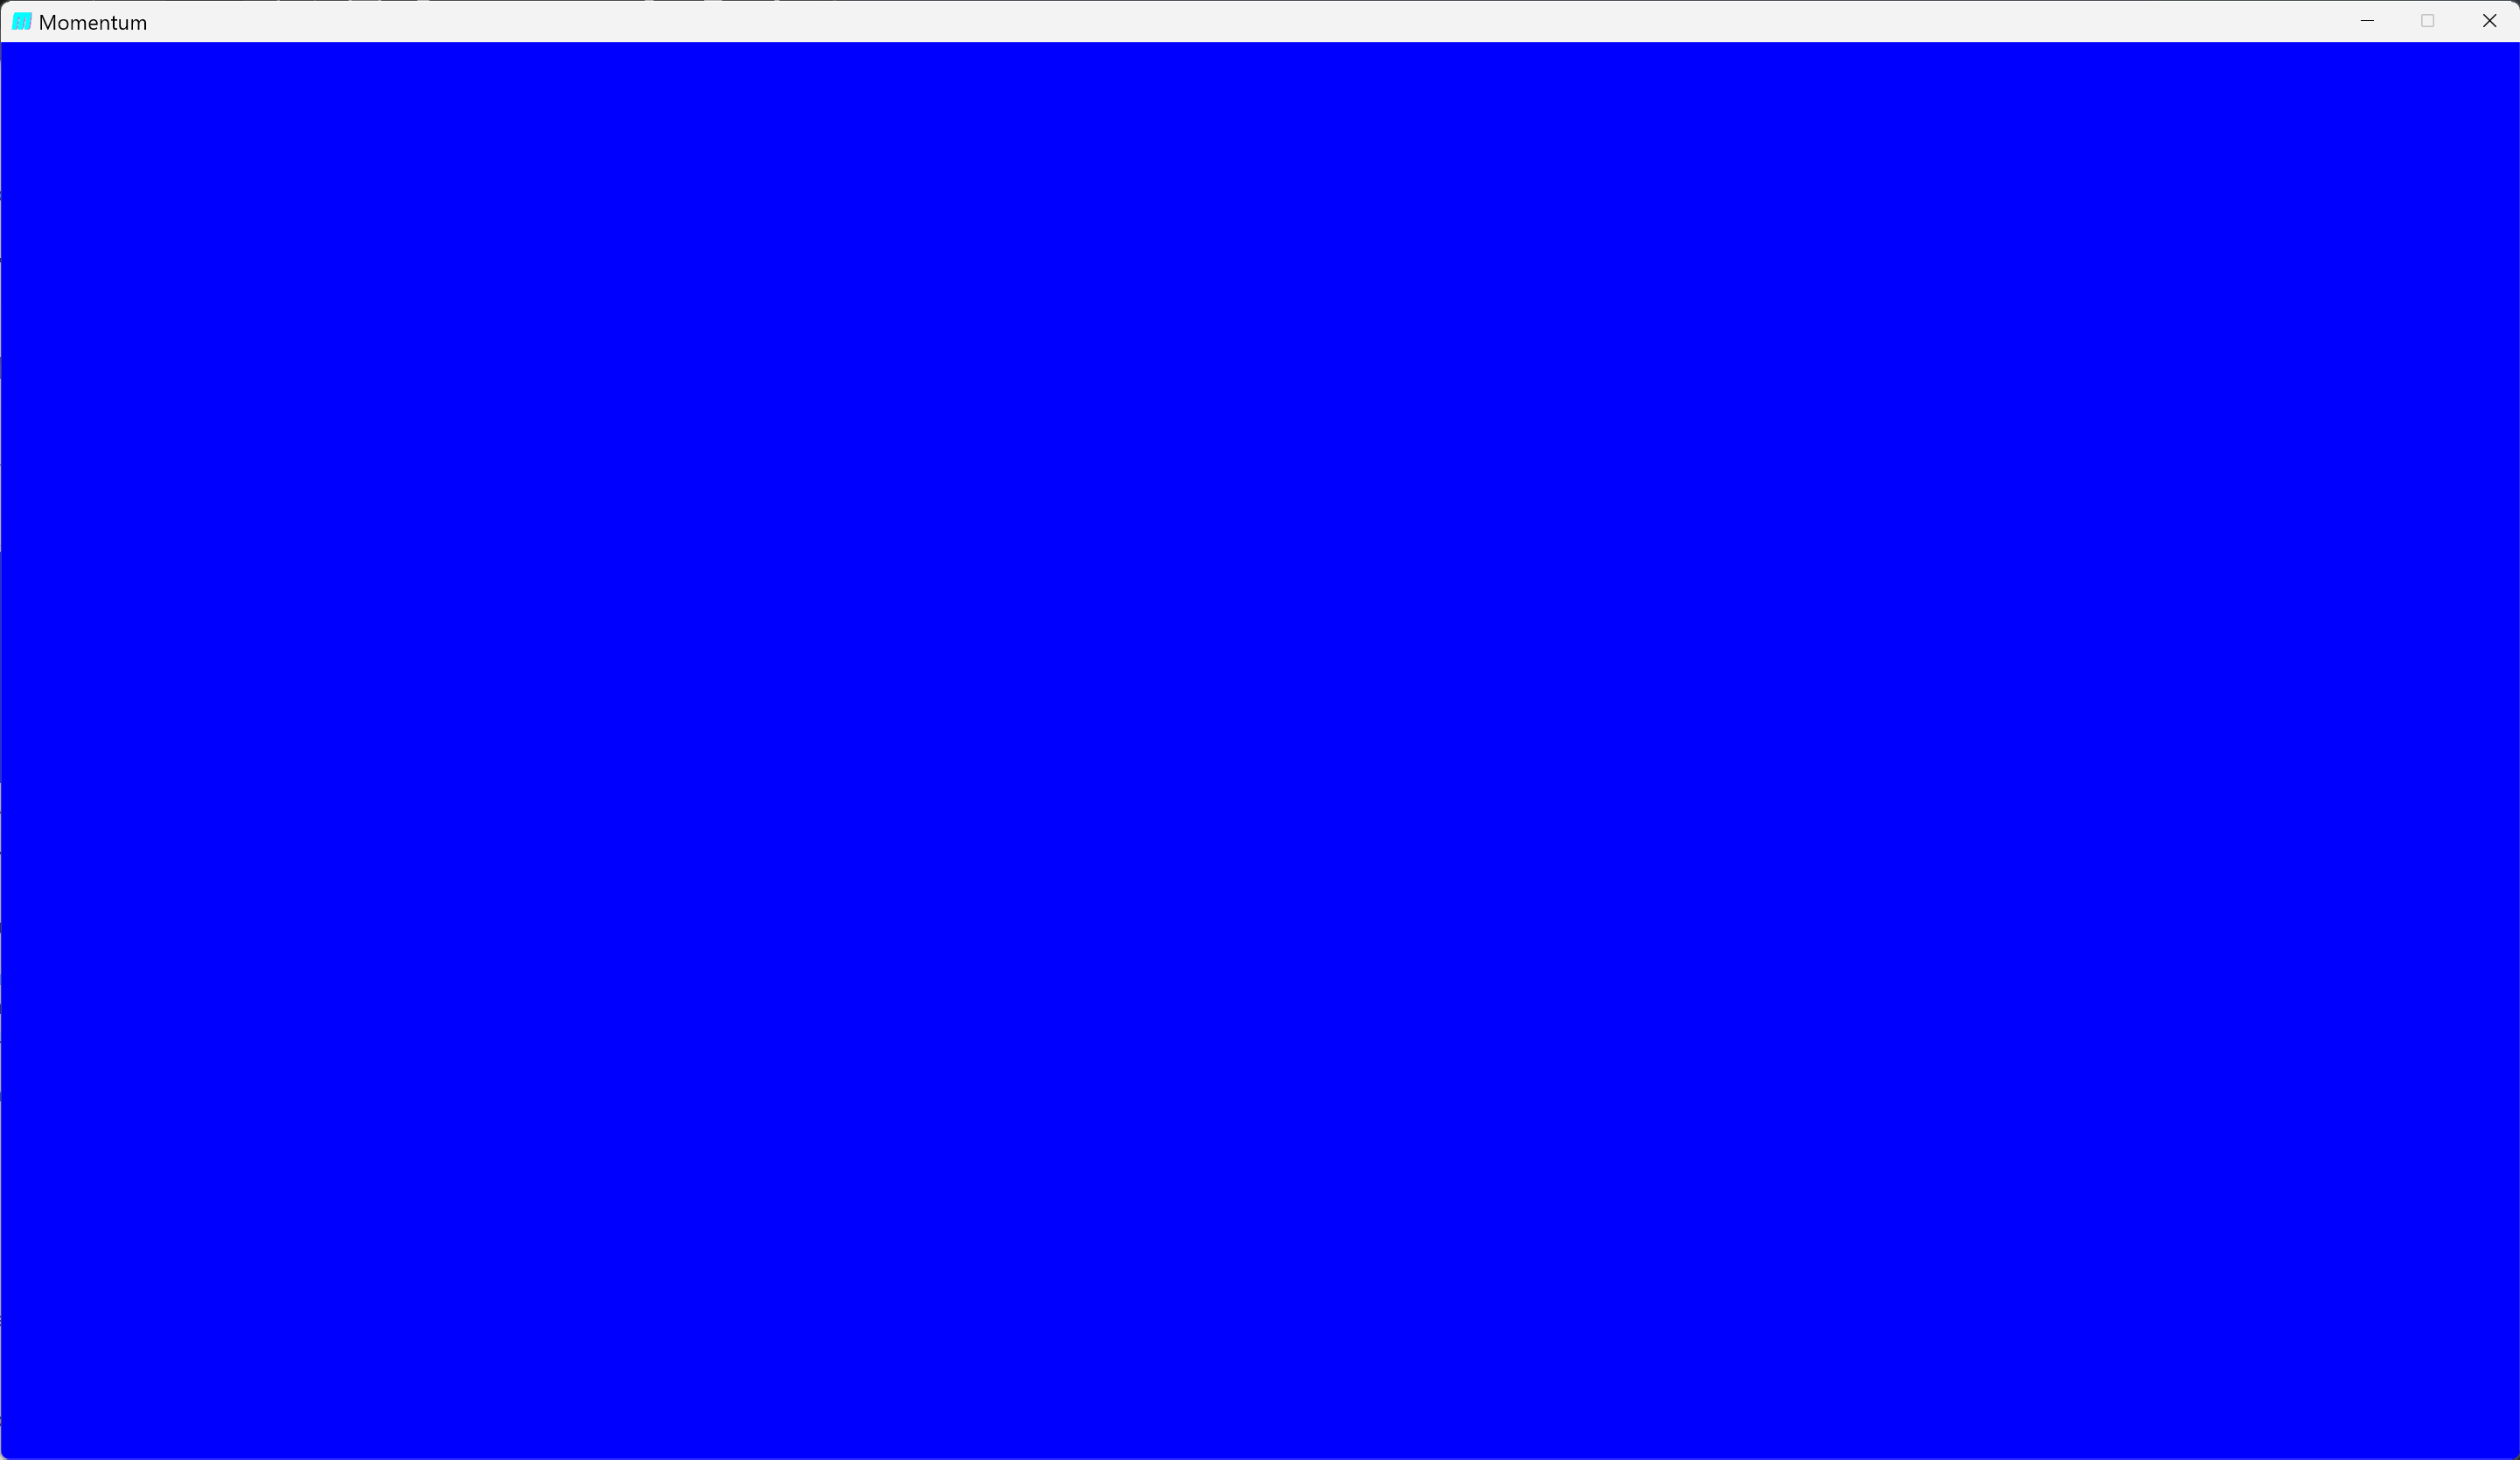
\includegraphics[width = \textwidth]{Development/Images/MenuA.png}
    \caption{Menu A}
    \label{fig:menu_a}
    \end{subfigure}
    \begin{subfigure}{0.49\textwidth}
    \centering
    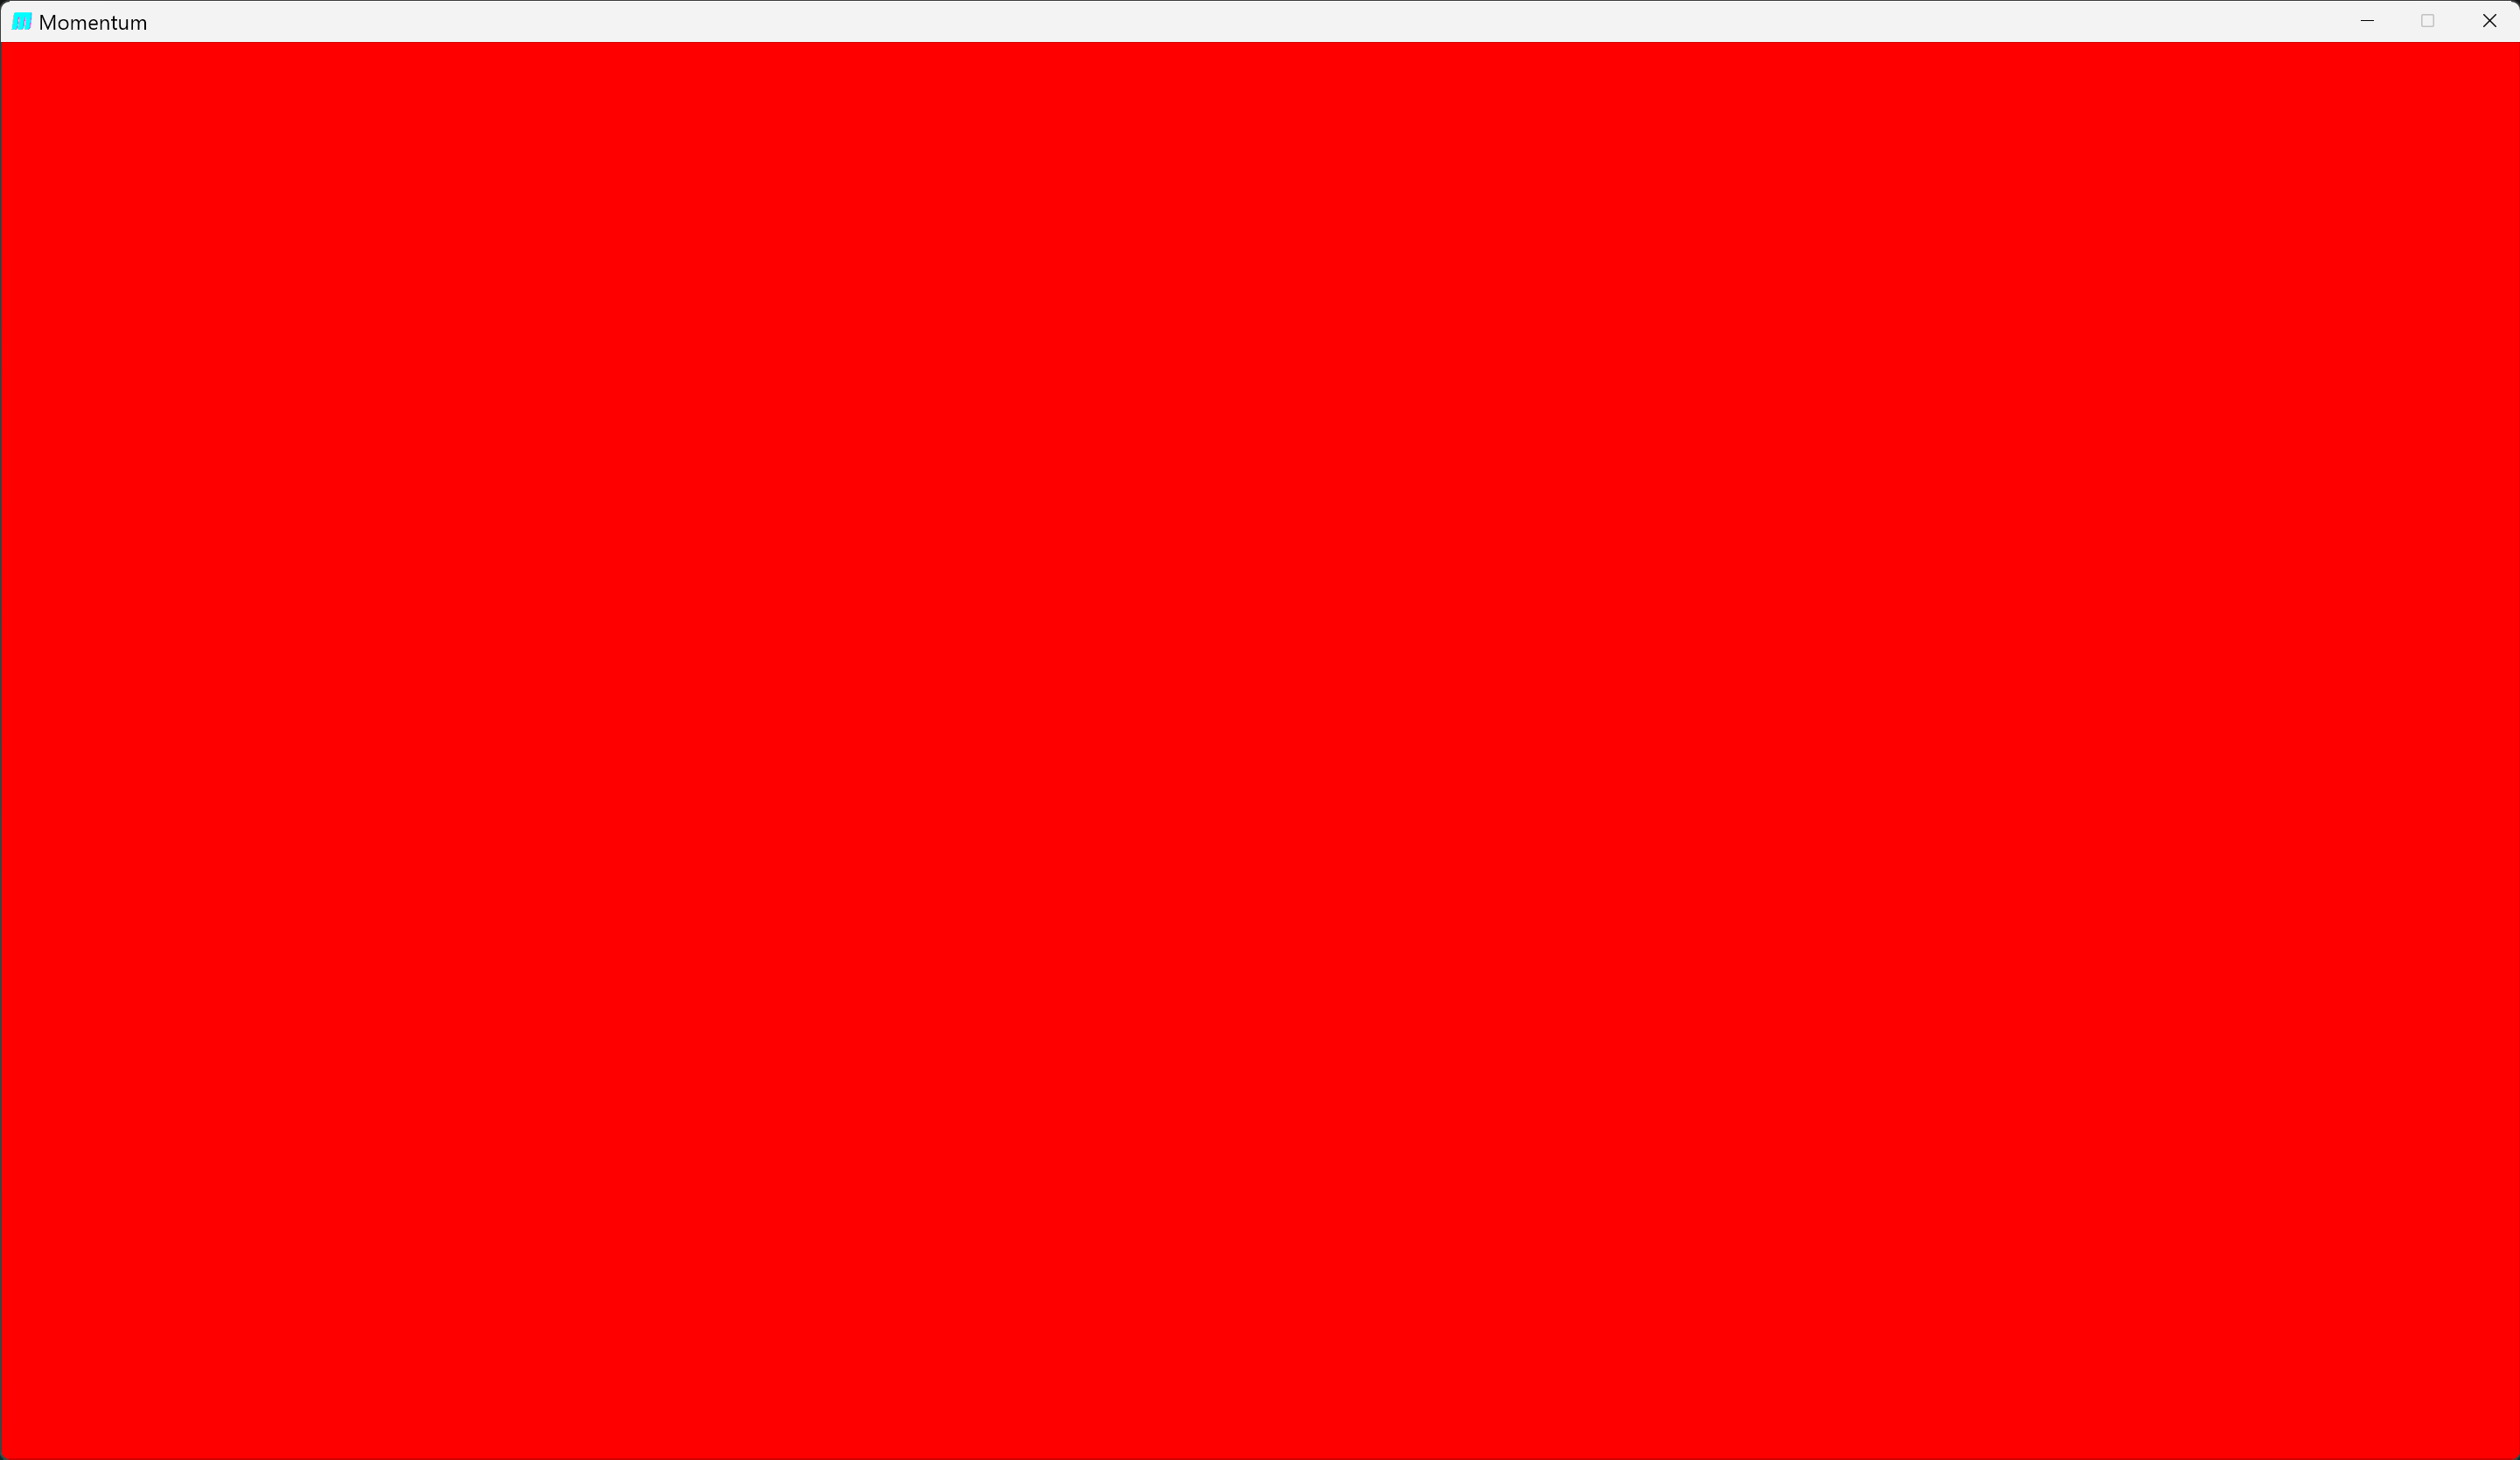
\includegraphics[width = \textwidth]{Development/Images/MenuB.png}
    \caption{Menu B}
    \label{fig:menu_b}
  \end{subfigure}
  \caption{Screen captures from the two menus.}
  \label{fig:menu_ab}
\end{figure}

\vs
We will take the start menu and the login menu to begin with. Each one of these classes will have some text on the screen. We will create the Start Menu first, and then we can show that we can move between them, thus proving that the \m{Game} class works at switching between different states. The first thing we will do is import \m{pygame.FreeType} at the start of \m{menu.py}. We will also create our font object here.


\begin{mpy}
import pygame.freetype

#Initalise freetype
pygame.freetype.init()

#Create text font
text_font = pygame.freetype.SysFont('iosevka', 64)
\end{mpy}

\vs
After this, we need to create our \m{Start} class, which is done as follows. We create our constructor as follows. We need to set our display so that the menu can rende.

\begin{mpy}
#Directed from the login page
class Start:
    def __init__(self, display, gameStateManager):
        #Set the display on which we are rendering
        self.display = display
        
        #Set the gsm
        self.gameStateManager = gameStateManager

        #Set screen dims
        self.SCREEN_DIMS = gameStateManager.SCREEN_DIMS

        #Set bg color
        self.BG_COLOR = (0, 255, 255)
\end{mpy}

\vs
The next part of the code is the running of the menu itself. Here, we will be filling the display with a certain colour, and then writing some text onto it. We set the bounding rectangle to have a centre at the centre of the screen, so that we can align the text nicely. We then check to see if the user wants to quit the game and if not, we repeat the loop until they do. This code was partially constructed with help from \href{https://stackoverflow.com/questions/23982907/how-to-center-text-in-pygame}{this link}.

\vs
\begin{mpy}
  def run(self, returnValues):

    #Fill display
    self.display.fill(self.BG_COLOR)

    #Create clock
    self.clock = pygame.time.Clock()
    dt = 0

    #Initialise variables
    #TODO: SHOULD BE MOVED INSIDE THIS IS A BUG PLEASE DOCUMENT IT
    inPos = False
    running = True
    clicked = False

    #Main loop
    while running:

      #Redraw display
      self.display.fill(self.BG_COLOR)

      #Render text
      text_surface, text_rect = text_font.render('Start Menu', fgcolor=(0, 0, 0), bgcolor=self.BG_COLOR)
      text_rect.center = (self.SCREEN_DIMS[0] // 2, self.SCREEN_DIMS[1] // 2)

      #Blit to surface
      self.display.blit(text_surface, text_rect)

      # Get all events
      events = pygame.event.get()

      # Get all key presses
      keys = pygame.key.get_pressed()
      
      for event in events:

          # Check if user wants to quit
          if event.type == pygame.QUIT:
              pygame.quit()
              sys.exit()

      #Update the display
      pygame.display.update()

      #Tick the clock
      dt = self.clock.tick(self.gameStateManager.REFRESH_RATE)
        
    return returnValues
\end{mpy}

\vs
We also need to change the initial value of the game state manager's state from \m{'game_loop'} to \m{'start'}. Having done this, we get the following image (Figure \ref{start_menu}) on the screen.

\begin{figure}[H]
    \centering
    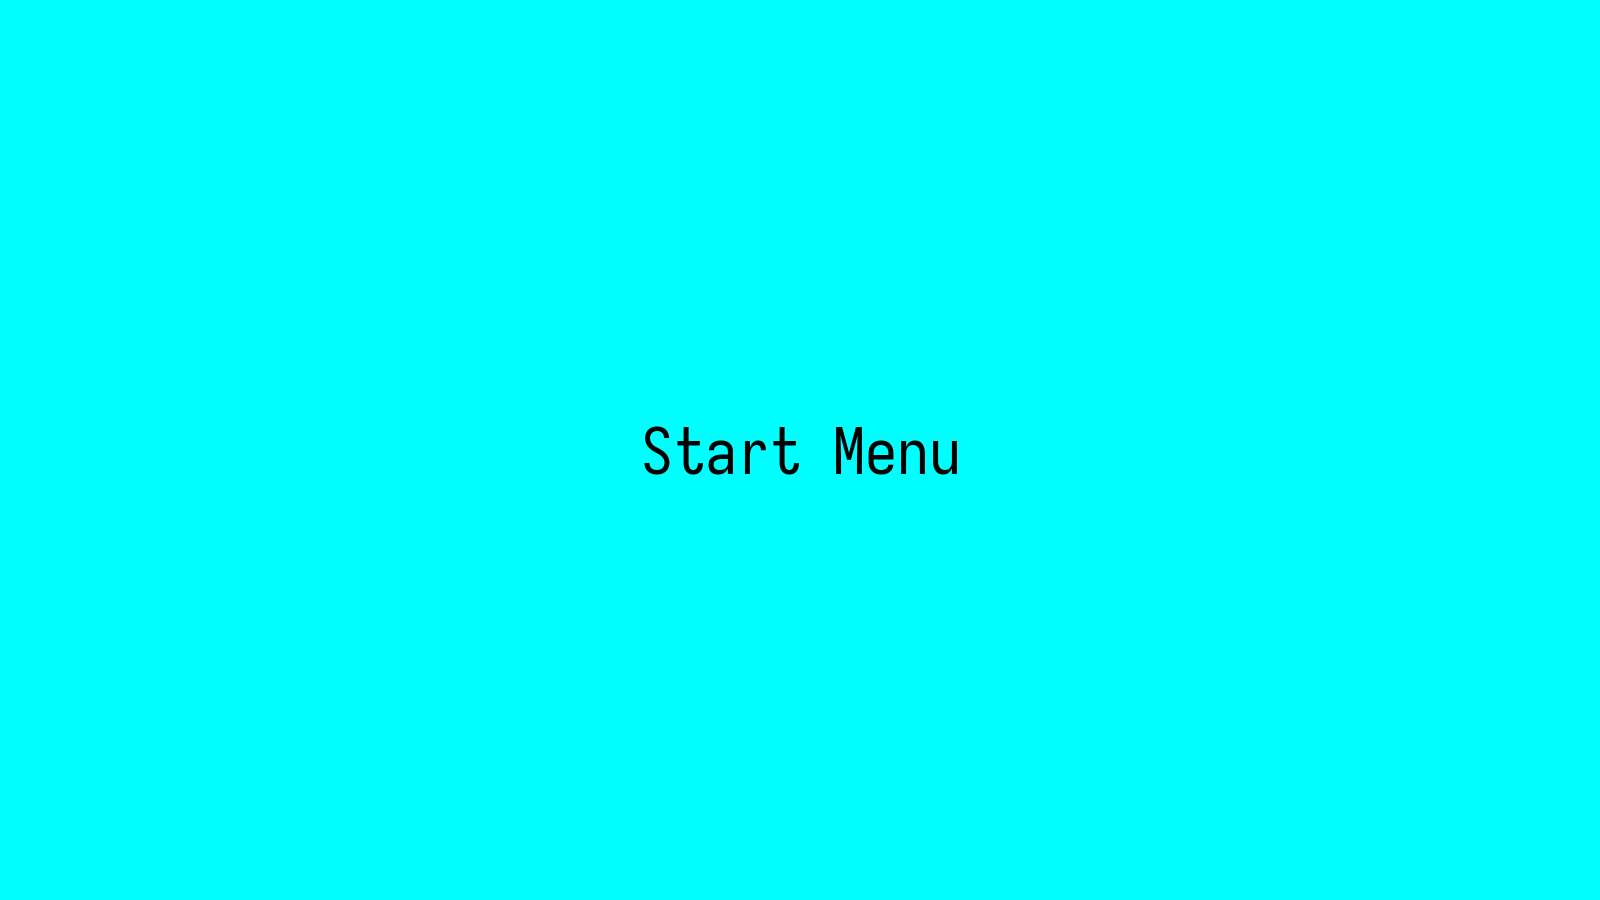
\includegraphics[width=\linewidth]{Development/Images/start_menu.png}
    \caption{An image capture of the start menu screen so far}
    \label{fig:start_menu}
\end{figure}
We can now take inputs from the keyboard and assign actions to them. Specifically, if the user presses a certain button we want to change the state of the \m{GameStateManager} using the setter method and then we want to set the inner loop to stop running so that we can go back to the outer loop and join the new state.

\vs
We can assign the up arrow to be the keyboard event to change the state. This is done as follows.

\begin{mpy}
      if keys[K_UP]:
          self.gameStateManager.setState('game_loop')
          running = False
\end{mpy}

This then means that we can switch to the main game loop immediately after pressing the up arrow key. We will introduce a delay, so that if the holds the arrow key for multiple frames this doesn't cause it to skip through menus. This will prevent them from accidentally skipping through important menus. Alternatively, we could use also use buttons in the menu, and only register when the user has pressed one of the mouse buttons. This will mean that we no longer need to use any delays, since the user will then have likely intentionally clicked on the button that they wanted to click on. Therefore, it would be useful to implement a button class, which we will do later. We will now show a video demonstrating this in action, although the keyboard inputs are not visible. The only input I gave to the system was the up and down arrow keys. However, since we don't have a game loop yet, this is a bit pointless. This is something we will rectify once we have a game loop.

\subsection{\textcolor{red}{Button}}

We will be implementing a \m{Button} class which we mentioned before. This will allow us to more easily use the menu system which we created in the previous section. As mentioned in the Design section, the button is just a rectangle over which we want to check if there has been any clicks. If there has been a click, then we take some action, such as leaving the game, or changing the state. This can be done as follows. We will inherit from the \m{Block} class, since this already implements some important features. Additionally, the \m{Rect} class in \m{PyGame} already implements a collide point method, so we can use that to see whether the position where the mouse has clicked is inside of the rectangle. We will write the constructor as follows.

\begin{mpy}
class Button(Block):

  def __init__(self, centre, length0, length2, colour, SCREEN_DIMS, text, bg_color):
    
    #Middle of the screen
    camera_position = U.mult(SCREEN_DIMS, 0.5)

    #Position as an integer
    camera_position = [int(i) for i in camera_position]

    #Initiate the block class in the 
    super(Button, self).__init__(centre, length0, length2, colour, SCREEN_DIMS, camera_position)

    #Set the bg color
    self.BG_COLOR = bg_color

    #Set the text surface and rect to write on
    self.text_surface, self.text_rect = text_font.render('Start Menu', fgcolor=(0, 0, 0), bgcolor=self.BG_COLOR)

    #Set the centre of the button on the screen
    self.text_rect.center = self.centre

    #Set screen dims for rendering
    self.SCREEN_DIMS = SCREEN_DIMS
\end{mpy}

We set the camera position to be in the middle of the screen, which means that we don't need to adjust our render functions, and we can just use this as our camera position, since we won't be moving anyway.

\vs
We will now write the render function as follows.

\begin{mpy}

  #Modified render function of the button
  def render(self, display, dt):

    #Render the rectange
    super().render(display, U.mult(self.SCREEN_DIMS, 0.5), [0, 0], dt, self.SCREEN_DIMS)

    #Render the text on top
    display.blit(self.text_surface, self.text_rect)
\end{mpy}

\href{https://stackoverflow.com/questions/23982907/how-to-center-text-in-pygame}{This was an important link, and we need to reference it}. We will now change the \m{Start} menu class to make use of this new button. We begin by adding the following lines to the constructor.

\vs
\begin{mpy}
    #Create button instance to use
    self.button = Button(U.mult(self.SCREEN_DIMS, 0.5), 350, 80, self.BG_COLOR, self.SCREEN_DIMS, "hello", self.BG_COLOR)
\end{mpy}

This ensures that we can now use the button object inside of the main loop. However, as of right now, it doesn't have any functionality, so we will implement a click function which will tell us when the mouse cursor is over the button. We can then find when the mouse button is clicked and if both conditions are met then the button has been clicked. In the \m{Button} class we can add a new function.

\tbc


\subsection{\textcolor{blue}{Game Loop}}

We will be creating a new class \m{GameLoop}, which will be running the game loop. To do this, we will be taking the \m{display} which we need to work on, the \m{GameStateManager}, and then we can assign all of the characteristics from this to the class in order to make them even easier to access.
\vs
\begin{mpy}
class GameLoop:

  def __init__(self, display, gameStateManager):

    #Get the display we are working on
    self.display = display

    #Get the gameStateManager, so we can process it within the class
    self.gameStateManager = gameStateManager

    #Get the screen dimensions conveniently
    self.SCREEN_DIMS = self.gameStateManager.SCREEN_DIMS
\end{mpy}

\vs
We also need to initialise a new clock and set \m{dt} in order to be able to use frame-rate independent physics. We have currently set a place holder on the initial position of the player until we set up spawn points, teams, etc.

\vs

\begin{mpy}
    #Placeholders for the moment
    self.pos_x = self.SCREEN_DIMS[0]//2
    self.pos_y = self.SCREEN_DIMS[1]//2

    #Initialise the clock, and set the refresh rate
    self.clock = pygame.time.Clock()
    self.REFRESH_RATE = self.gameStateManager.REFRESH_RATE
\end{mpy}
\vs
We need to create an actual game loop. Specifically, we need to contain this game loop inside of a run function, since all of the game state objects will contain a \m{run()} function that will be called everytime we are changing states. 
\begin{mpy}
  def run(self, returnValues):

    dt = 0

    player1 = Player([self.pos_x, self.pos_y], [0, -1], 0, 'empty')

    #List of all players
    self.players = [player1]

    running = True

    while running:

      self.display.fill((255, 255, 255))

      #Check if player wants to quit
      for event in pygame.event.get():
        if event.type == pygame.QUIT:
          pygame.quit()
          sys.exit()

      #Get the key presses and mouse position and buttons
      keys = pygame.key.get_pressed()

      mouse_pos = pygame.mouse.get_pos()

      mouse_clicks = pygame.mouse.get_pressed()

      #Get direction vector
      player1_direction = [mouse_pos[0] - self.SCREEN_DIMS[0]//2, mouse_pos[1] - self.SCREEN_DIMS[1]//2]

      #Normalise direction vector
      dir_mag = sqrt(sum([i**2 for i in player1_direction]))
      player1_direction = [i / dir_mag for i in player1_direction]

      #Update the direction vector
      player1.forward_vec = player1_direction

      #Get the directions which are pressed
      directions = [int(keys[K_d]), int(keys[K_a]), int(keys[K_s]), int(keys[K_w])]

      for player in self.players:
          player.render(self.display, player1.position, directions, dt, self.SCREEN_DIMS)

      #Update the display
      pygame.display.update()

      #Tick the clock
      dt = self.clock.tick(self.REFRESH_RATE)/1000

    return None
\end{mpy}

We will now re-write the \m{render()} function in the \m{Player} class, since there is a lot of ineffecienies in the way it was written, and now that the \m{Utility} class is available we can make the code a lot more efficient, readable, and maintainable. Additionally, there were a lot of values that were being calculated twice, and now we can get rid of that. This produces the following code.
\vs

\begin{mpy}
  #Renders the character to the display of the player
  def render(self, display, camera_position, directions, dt, SCREEN_DIMS):

    #Find relative posistion
    rel_pos = U.convertToScreen(camera_position, self.position, SCREEN_DIMS)

    #Draw the circle
    pygame.draw.circle(display, self.colour, rel_pos, self.radius)

    #Final extent of the forward vector
    for_pos = U.vecAdd(U.mult(self.forward_vec, 100), rel_pos)

    #Draw anti-aliased line for forward vector
    pygame.draw.aaline(display, (0, 0, 0), rel_pos, for_pos)

    #Move the player
    self.movePlayer(directions, dt)
\end{mpy}



Setting the start state to be \m{"game_loop"}, we can only see a blank screen. This is because we aren't drawing anything to the screen. Therefore, we need to add the \m{render()} function to the main loop. Whilst we are doing that, we can also add a block, since the player will just be stationary in the middle of the screen. We start by adding the block to the section before the \m{while} loop in the \m{run()} function.

\begin{mpy}
    block1 = Block([self.pos_x, self.pos_y + 200], 100, 200, (100, 0, 0), self.SCREEN_DIMS, player1.position)

    #List of all blocks
    blocks = [block1]
\end{mpy}

Then, we add the following lines of code in the \m{while} loop, as shown below. The first and last lines are already present, but were added for clarity. This will now render both the player and the block.

\begin{mpy}
      #Get the directions which are pressed
      directions = [int(keys[K_d]), int(keys[K_a]), int(keys[K_s]), int(keys[K_w])]

      for player in players:
        player.render(self.display, player1.position, directions, dt, self.SCREEN_DIMS)

      for block in blocks:
        block.render(self.display, player1.position, directions, dt, self.SCREEN_DIMS)

      #Update the display
      pygame.display.update()
\end{mpy}

This results in the output shown below.

\begin{figure}[H]
    \centering
    {
    \setlength{\fboxsep}{0pt}%
    \setlength{\fboxrule}{1pt}%
    \fbox{
\includegraphics[width=\linewidth]{Development/Images/game_loop_1.png}}
    }
    \caption{An image capture of the game loop}
    \label{fig:game_loop_1}
\end{figure}

Here is a \href{https://youtu.be/ICvIX3ar_eY}{video} demonstrating what this looks like. Both keyboard and mouse inputs were given here.

\vs
We can now add more players and more blocks into the map in order to make the game loop more alike to a real game setting. This is done simply by adding more player instances at different positions. For now, we will set the players to be in the top left corner of the map, and at regularly space intervals. We also want to be able to differentiate between the two teams, so we add this bit of code into the constructor for \m{Player}. This will allow us to choose colours based on which team the player is in.

\begin{mpy}
    self.colours = {0: (0, 100, 100),
                    1: (100, 20, 0)
                    }

    self.colour = self.colours[team]
\end{mpy}

Now that we have this, we can add the players as follows.

\begin{mpy}
    # Team 1
    player1 = Player([self.pos_x - 500, self.pos_y + 400], [0, -1], 0, Shotgun())
    player2 = Player([self.pos_x, self.pos_y + 400], [0, -1], 0, AssaultRifle()
    )
    player3 = Player([self.pos_x + 500, self.pos_y + 400], [0, -1], 0, SniperRifle()
    )

    # Team 2
    player4 = Player([self.pos_x - 500, self.pos_y], [0, 1], 1, Shotgun())
    player5 = Player([self.pos_x, self.pos_y], [0, 1], 1, AssaultRifle())
    player6 = Player([self.pos_x + 500, self.pos_y], [0, 1], 1, SniperRifle())

    # Contains all of the players in the game
    self.players = [player1, player2, player3, player4, player5, player6]
\end{mpy}

We will temporarily remove the block from the scene, and add it back later. We still need to make one more change however. Since the other players will be controlled with AI, we need to find some way of getting inputs to the other players. To do this, we will be using a list containing all of the inputs to the other players. We will set one of these inputs to be the human input, which will then control \m{player1}. To do this efficiently, we will use the \m{enumerate} keyword in \m{Python}. This is written as follows.

\begin{mpy}
      #Output from the model will go here
      model_predictions = [
        directions,
        [0, 0, 0, 0],
        [0, 0, 0, 0],
        [0, 0, 0, 0],
        [0, 0, 0, 0],
        [0, 0, 0, 0],
      ]

      #Render and move players as needed
      for i, player in enumerate(players, 0):
        player.render(self.display, player1.position, model_predictions[i], dt, self.SCREEN_DIMS)
\end{mpy}

This appears as shown in Figure \ref{fig:game_loop_2}. \href{https://youtu.be/KU45hIX5U_0}{Here is a video} showing this in action.

\begin{figure}
  \centering
  \begin{subfigure}{0.49\textwidth}
    \centering
    {
    \setlength{\fboxsep}{0pt}%
    \setlength{\fboxrule}{1pt}%
    \fbox{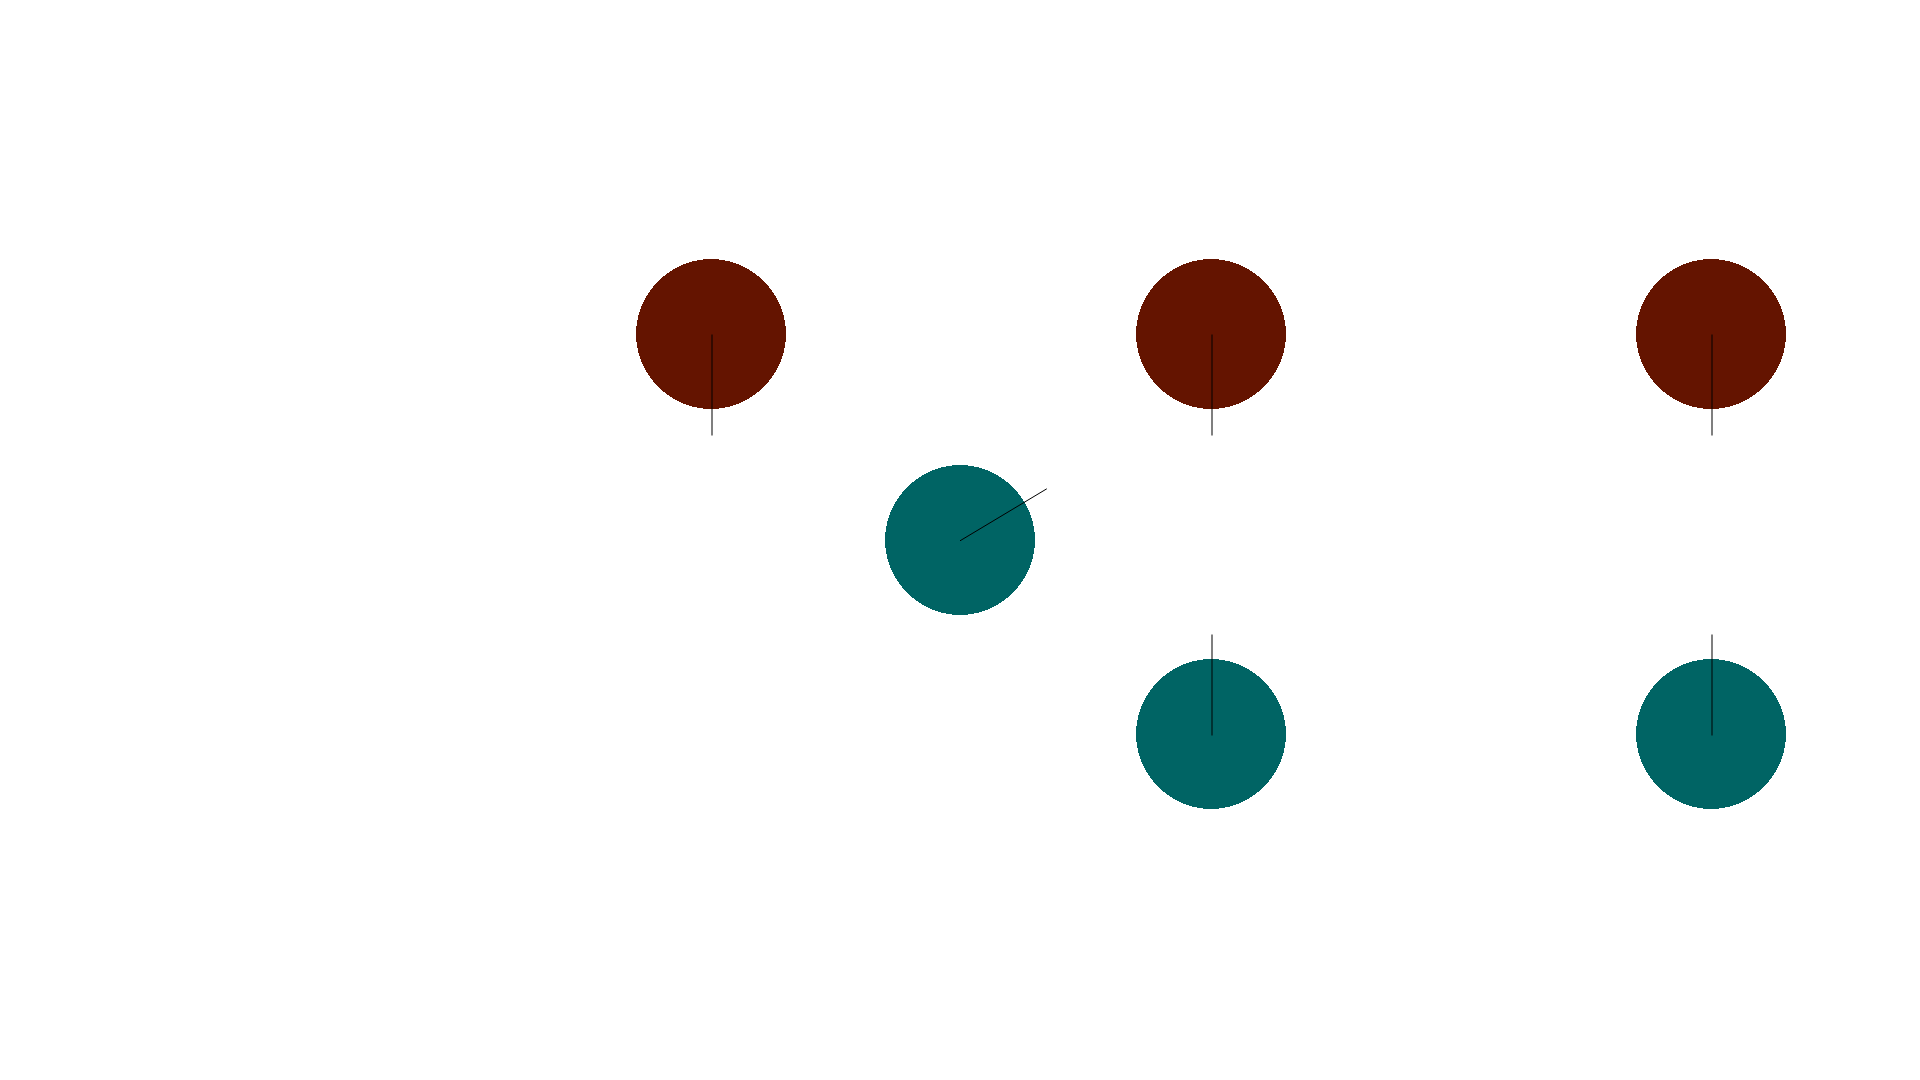
\includegraphics[width = \textwidth]{Development/Images/game_loop_2.png}}}
    \caption{Screen Capture 1}
    \label{fig:game_loop_2_1}
    \end{subfigure}
    \begin{subfigure}{0.49\textwidth}
    \centering
    {
    \setlength{\fboxsep}{0pt}%
    \setlength{\fboxrule}{1pt}%
    \fbox{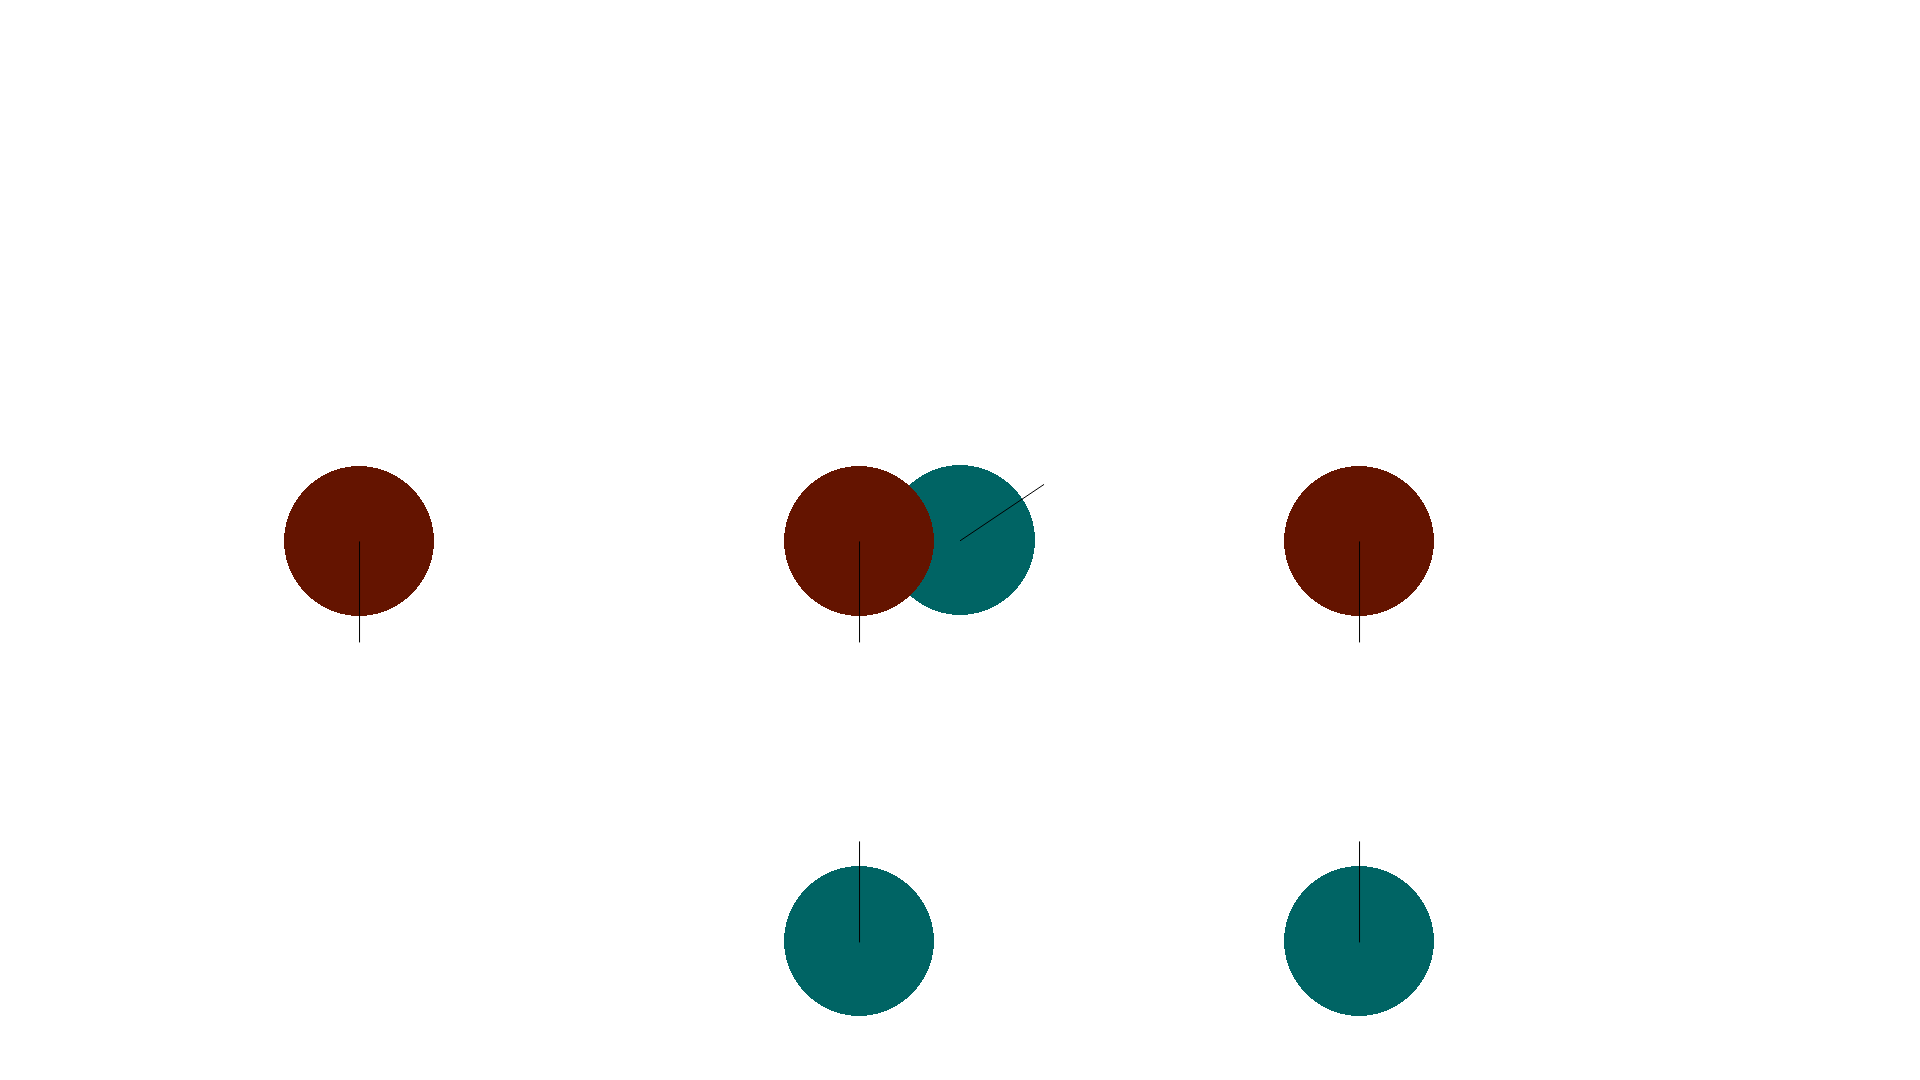
\includegraphics[width = \textwidth]{Development/Images/game_loop_2_b.png}}}
    \caption{Screen Capture 2}
    \label{fig:game_loop_2_2}
  \end{subfigure}
  \caption{Screen captures of two different states in the game loop.}
  \label{fig:game_loop_2}
\end{figure}

\vs
Then next thing we need to do is seperate the render function and the player update. This is important because we need to be able to manage the player states instead of moving it directly. Additionally, it is not the responsibility of the render function to do this. Therefore, we will create a new \m{updatePlayerState} which will take in the directions, and will update the player states.

\begin{mpy}
  def updatePlayerState(self, action, dt):
    #Move the player
    self.movePlayer(action, dt)
\end{mpy}

We will now remove the \m{directions} and \m{dt} inputs from the \m{render()} function since they are no longer needed. This gives the same outputs as shown above. Furthermore, we want to now change the way we are taking inputs. This is because they are based on convention and will make the output from the models harder to work with. Additionally, when we start working with the AI, it is difficult to get an output for the forward and backwards directions and similarly for horizontal inputs, since it is much easier to work with just a single value between -1 and 1. Therefore, we will update the move player function as follows.

\begin{mpy}
  def movePlayer(self, directions, dt):
    #directions = [horizontal input, vertical input]

    #Used to normalise directions
    magnitude = sqrt(U.dot(directions, directions))

    #If no movement, break
    if magnitude == 0:
        return None

    #Calculate movement in the frame
    frameMovement = U.mult(directions, (dt * self.max_speed)/magnitude)

    #Update position
    updatedPosition = U.vecAdd(self.position, frameMovement)

    #Position must be inside of the field
    for i in range(2):
        
      if updatedPosition[i] - self.radius <= 0:
        updatedPosition[i] = self.radius

      elif updatedPosition[i] + self.radius >= 8000:
        updatedPosition[i] = 8000 - self.radius

    #Set new position
    self.position = updatedPosition
\end{mpy}

However, there is still a problem with this code. This is because, if we put our input into the red team, we see that the inputs are still moving the same way they would for the blue team. This is shown in this \href{https://youtu.be/XTUu_KktHLQ}{video}.

However, this is not what we expect to see. The way to resolve this is to use the initial forward vector of the player. This is done as follows. We need to start by creating a right pointing vector in the constructor.

\begin{mpy}
    if self.initial_forward_vec == [0, -1]:
      self.initial_right_vec = [1, 0]
    else:
      self.inital_right_vec = [-1, 0]
\end{mpy}

However, there is still a more efficient way of doing this. The inputs are completely flipped for the opposite team, so we just need to multiply the input direction by -1 for the red team, and for 1 on the blue team. We can remove the right vector, since it is no longer required. We can add the following lines in the constructor.

\begin{mpy}
    if self.initial_forward_vec == [0, -1]:
      self.movement_multiplier = 1
    else:
      self.movement_multiplier = -1
\end{mpy}

Then, the movement is updated as follows.

\begin{mpy}
    #Calculate movement in the frame
    frameMovement = U.mult(directions, self.movement_multiplier * dt * self.max_speed/magnitude)
\end{mpy}

This then produces the output we expect, as shown \href{https://youtu.be/ZixPY08tVlE}{in this video}.
\vs

The model will output a dictionary of the inputs that it wants the player to take. Therefore, we will modify our code as follows. In the \m{run()} function, we want to edit the \m{model_predictions} to be as follows.

\begin{mpy}
      #Output from the model will go here
      model_predictions = [
        {"forward": directions[1], "right": directions[0], "rot_rate": 0},
        {"forward": 0, "right": 0, "rot_rate": 0},
        {"forward": 0, "right": 0, "rot_rate": 0},
        {"forward": 0, "right": 0, "rot_rate": 0},
        {"forward": 0, "right": 0, "rot_rate": 0},
        {"forward": 0, "right": 0, "rot_rate": 0},
      ]
\end{mpy}

In the \m{updatePlayerState()}, we do the following.

\begin{mpy}
  #Update the player state
  def updatePlayerState(self, action, dt):

    #Get the directions from the dictionary
    directions = [action["right"], action["forward"]]

    #Move the player
    self.movePlayer(directions, dt)
\end{mpy}

In the \m{run()} we also need to update the player state as follows. We will do this in a seperate loop, because we will also need to do state updates between the player movement update and the rendering.

\begin{mpy}
      #Update player states
      for i, player in enumerate(players, 0):
        player.updatePlayerState(model_predictions[i], dt)
\end{mpy}

We also need to rotate the direction vector. This is done as follows using the \m{U.rotateVec()} method we defined before. This is inserted into \m{updatePlayerState()}.

\begin{mpy}
    #If dt != 0 we want to turn
    if dt != 0:
      angleTurned = action["rot_rate"] * dt
      self.forward_vec = U.rotateVector(self.forward_vec, angleTurned)
\end{mpy}

We will also change the rotation rate for some of the characters. This will allow us to this in action.

\begin{mpy}
      #Output from the model will go here
      model_predictions = [
        {"forward": directions[1], "right": directions[0], "rot_rate": 0},
        {"forward": 0, "right": 0, "rot_rate": 1.5},
        {"forward": 0, "right": 0, "rot_rate": -1},
        {"forward": 0, "right": 0, "rot_rate": 1},
        {"forward": 0, "right": 0, "rot_rate": -1},
        {"forward": 0, "right": 0, "rot_rate": 0},
      ]
\end{mpy}

This produces the output as shown in Figure \ref{fig:game_loop_3_rot}, and also in \href{https://youtu.be/GxHD5rflfGw}{this video}.

\begin{figure}
  \centering
  \begin{subfigure}{0.49\textwidth}
    \centering
    {
    \setlength{\fboxsep}{0pt}%
    \setlength{\fboxrule}{1pt}%
    \fbox{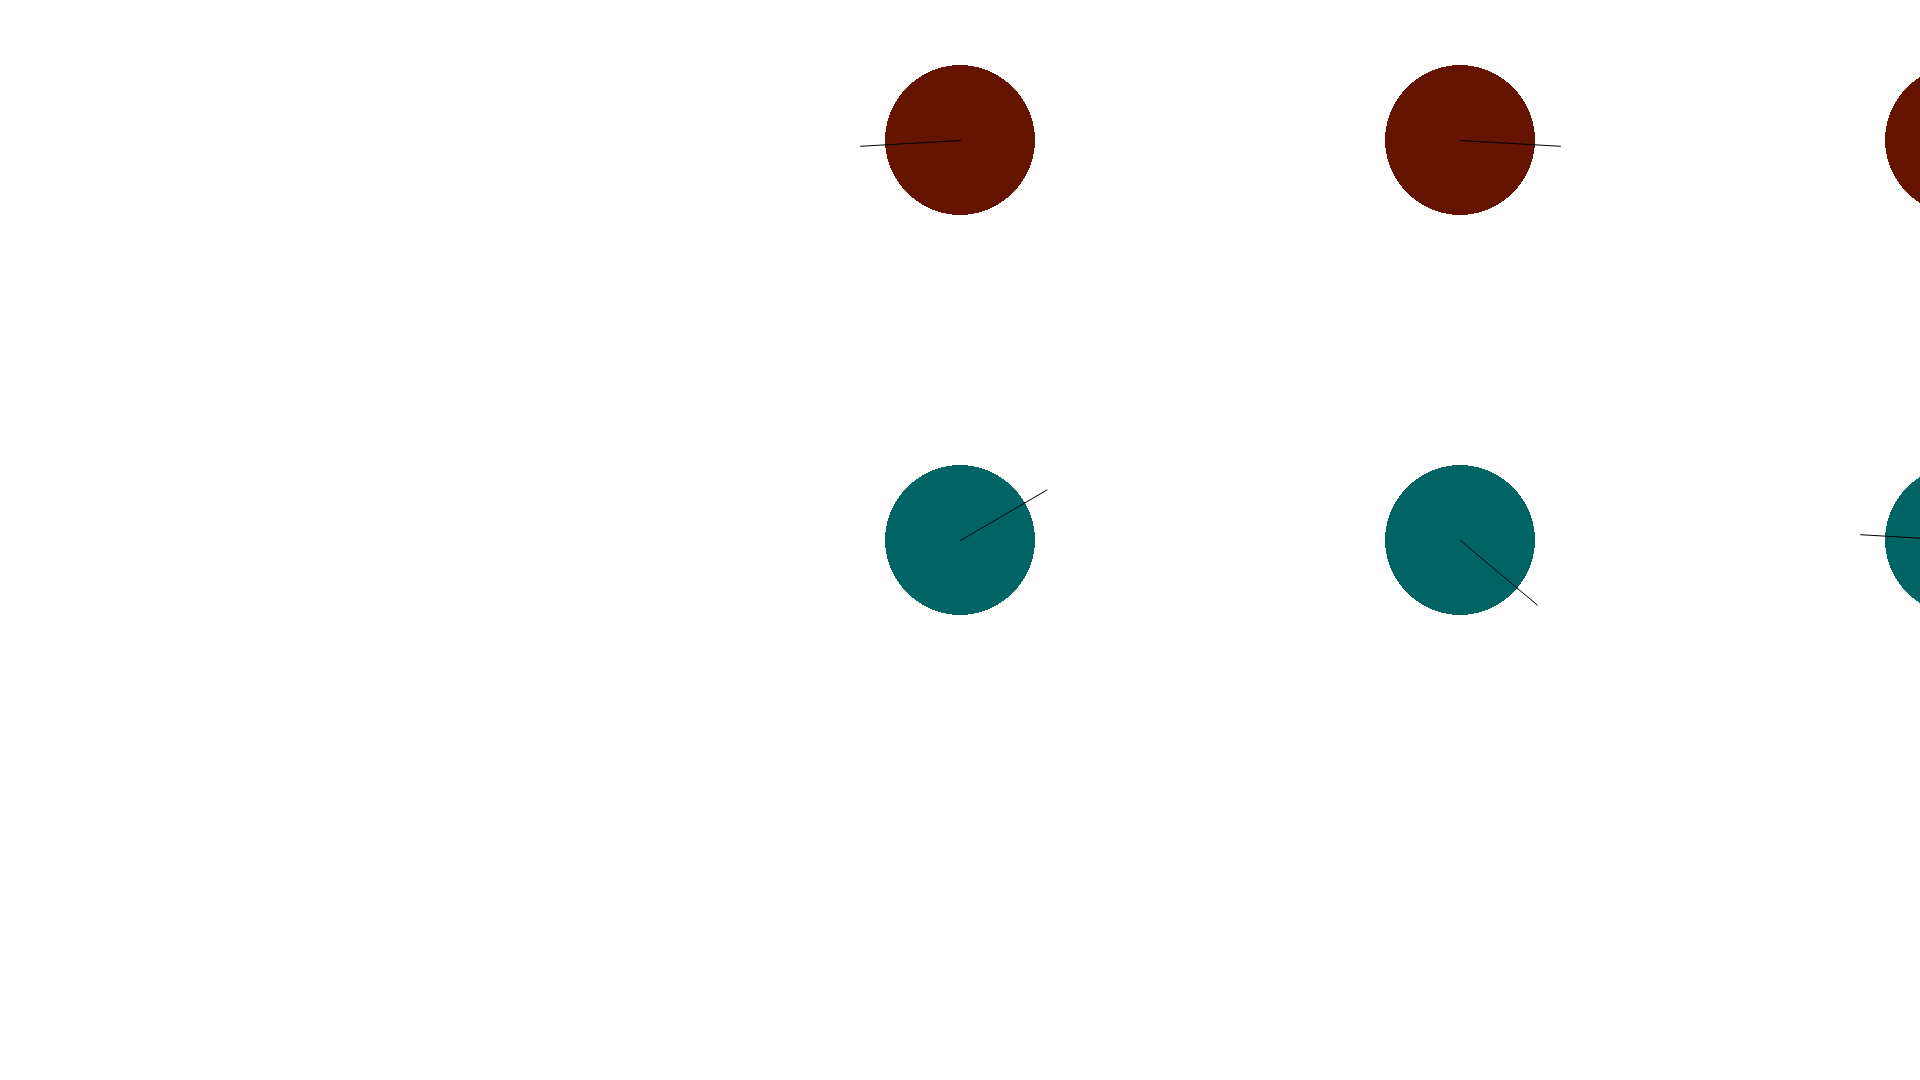
\includegraphics[width = \textwidth]{Development/Images/game_loop_3_a.png}}}
    \caption{Screen Capture 1}
    \label{fig:game_loop_3_1}
    \end{subfigure}
    \begin{subfigure}{0.49\textwidth}
    \centering
    {
    \setlength{\fboxsep}{0pt}%
    \setlength{\fboxrule}{1pt}%
    \fbox{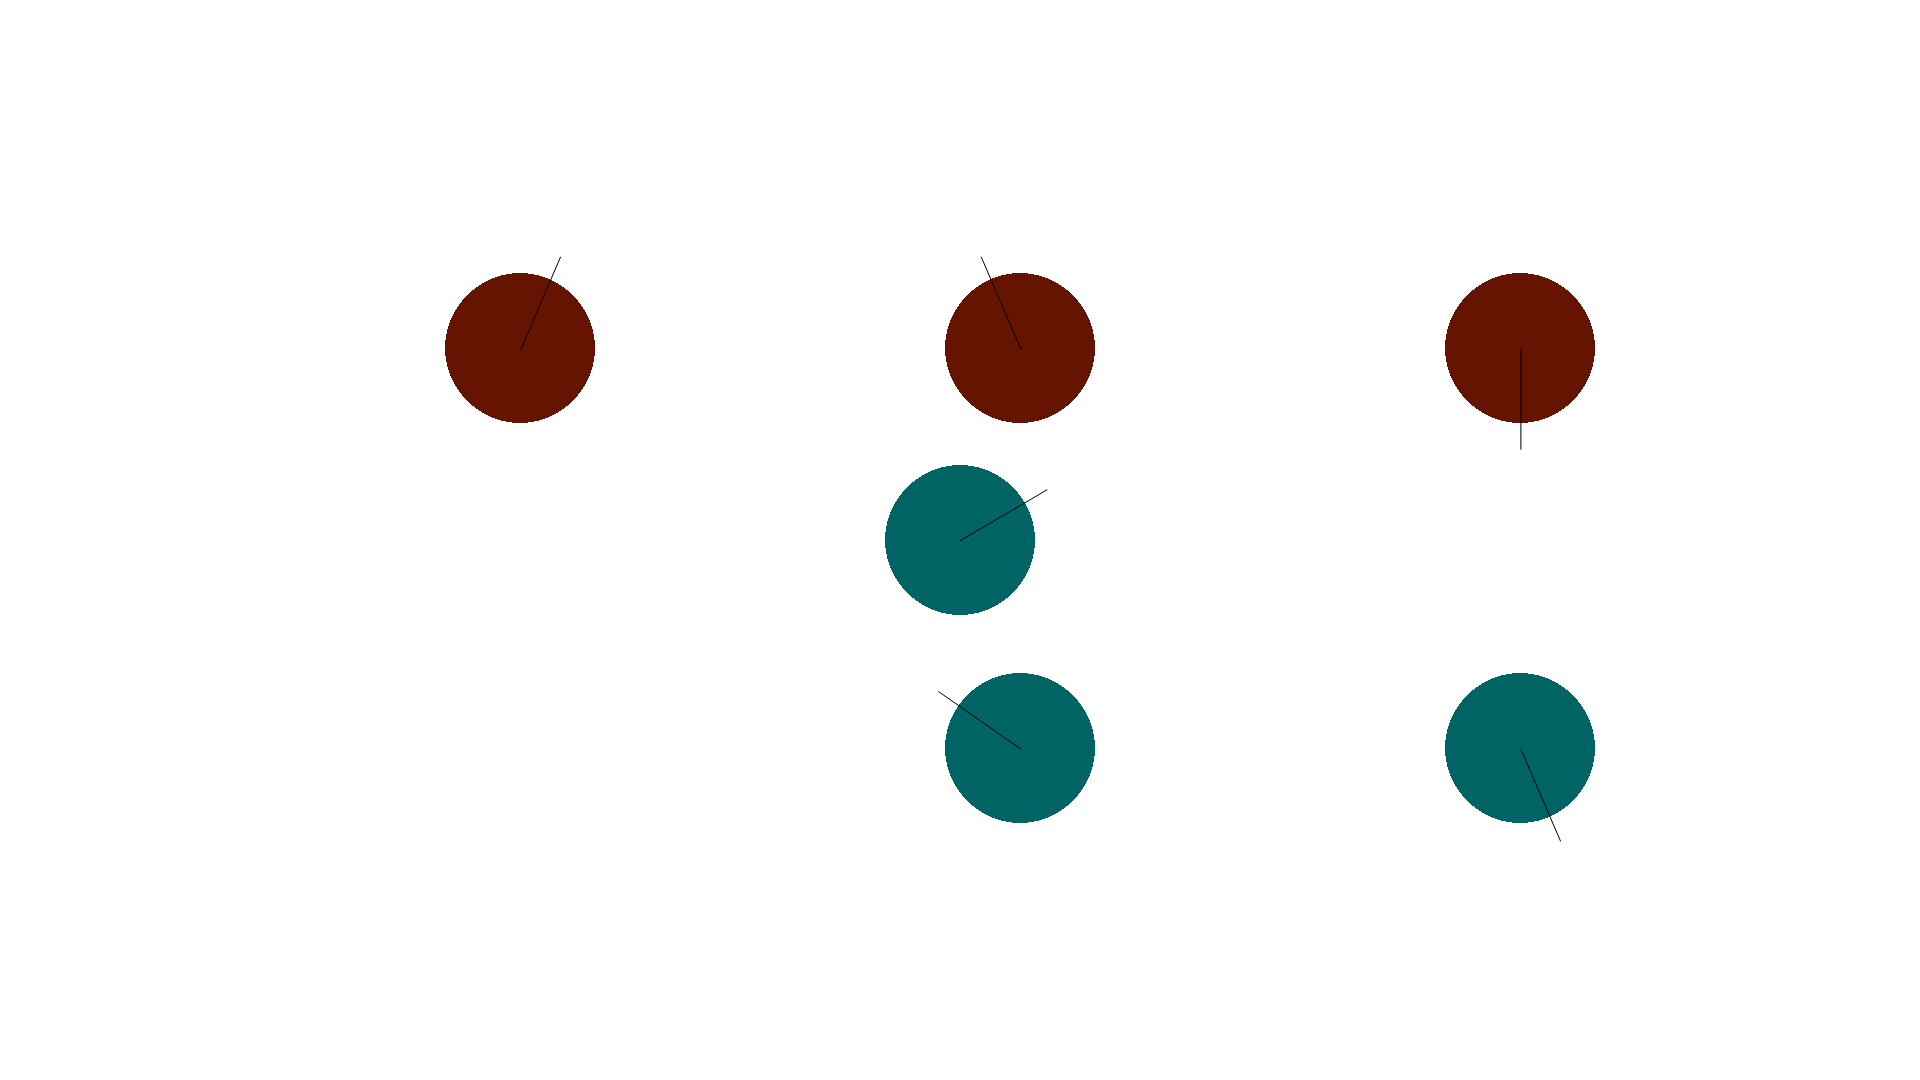
\includegraphics[width = \textwidth]{Development/Images/game_loop_3_b.png}}}
    \caption{Screen Capture 2}
    \label{fig:game_loop_3_2}
  \end{subfigure}
  \caption{Screen captures of two different states in the game loop whilst the players are rotating.}
  \label{fig:game_loop_3_rot}
\end{figure}

The next thing we want to do is to implement the firing system. This is the primary mechanic in the game, so it is important to implement it. To do this, we will need to setup a few things. Firstly, we need to take inputs for whether the player is firing or not. We can do this using another key in the inputs dictionary. We can also add an extra line in the \m{updatePlayerState()} to account for this. This is done as follows.
\begin{mpy}
    #Array of [Position, Final Extent, Damage]
    if action["firing"]:
      weaponRay = self.fire()
    else:
      weaponRay = []

    return weaponRay
\end{mpy}

We have not accounted for the cooldown of the weapon yet, but this is something we will implement in the next iteration of the weapon system. For now, we will need to update the main \m{run()} function. This is done as follows.

\begin{mpy}
      rays = {}
      #Update player states
      for i, player in enumerate(players, 0):
        rays[player] = player.updatePlayerState(model_predictions[i], dt)
\end{mpy}

We will also create a new function \m{handlesRayCollisions()} to deal with all of the rays that are being fired.

\begin{mpy}

\end{mpy}

In order to make the damage on the players more clear, we can display the health of the player on them. This will make the code easier to debug, and will show the player the health of the enemy. We add the following code to the start of the \m{player.py} file.

\begin{mpy}
import pygame.freetype

pygame.freetype.init()
text_font = pygame.freetype.SysFont('iosevka', 48)
\end{mpy}

In the render function, we add the following lines at the end.

\begin{mpy}
        #Create text surface of the health
        self.text_surface, self.text_rect = text_font.render(str(self.health), fgcolor=(255,255,255), bgcolor=self.colour)

        #Set text position
        self.text_rect.center = rel_pos

        #Blit the text
        display.blit(self.text_surface, self.text_rect)
\end{mpy}

This will create the text surface, and will draw it onto the screen. The screen capture of the game is shown in \ref{fig:game_loop_4}.

\begin{figure}[H]
    \centering
    {
    \setlength{\fboxsep}{0pt}%
    \setlength{\fboxrule}{1pt}%
    \fbox{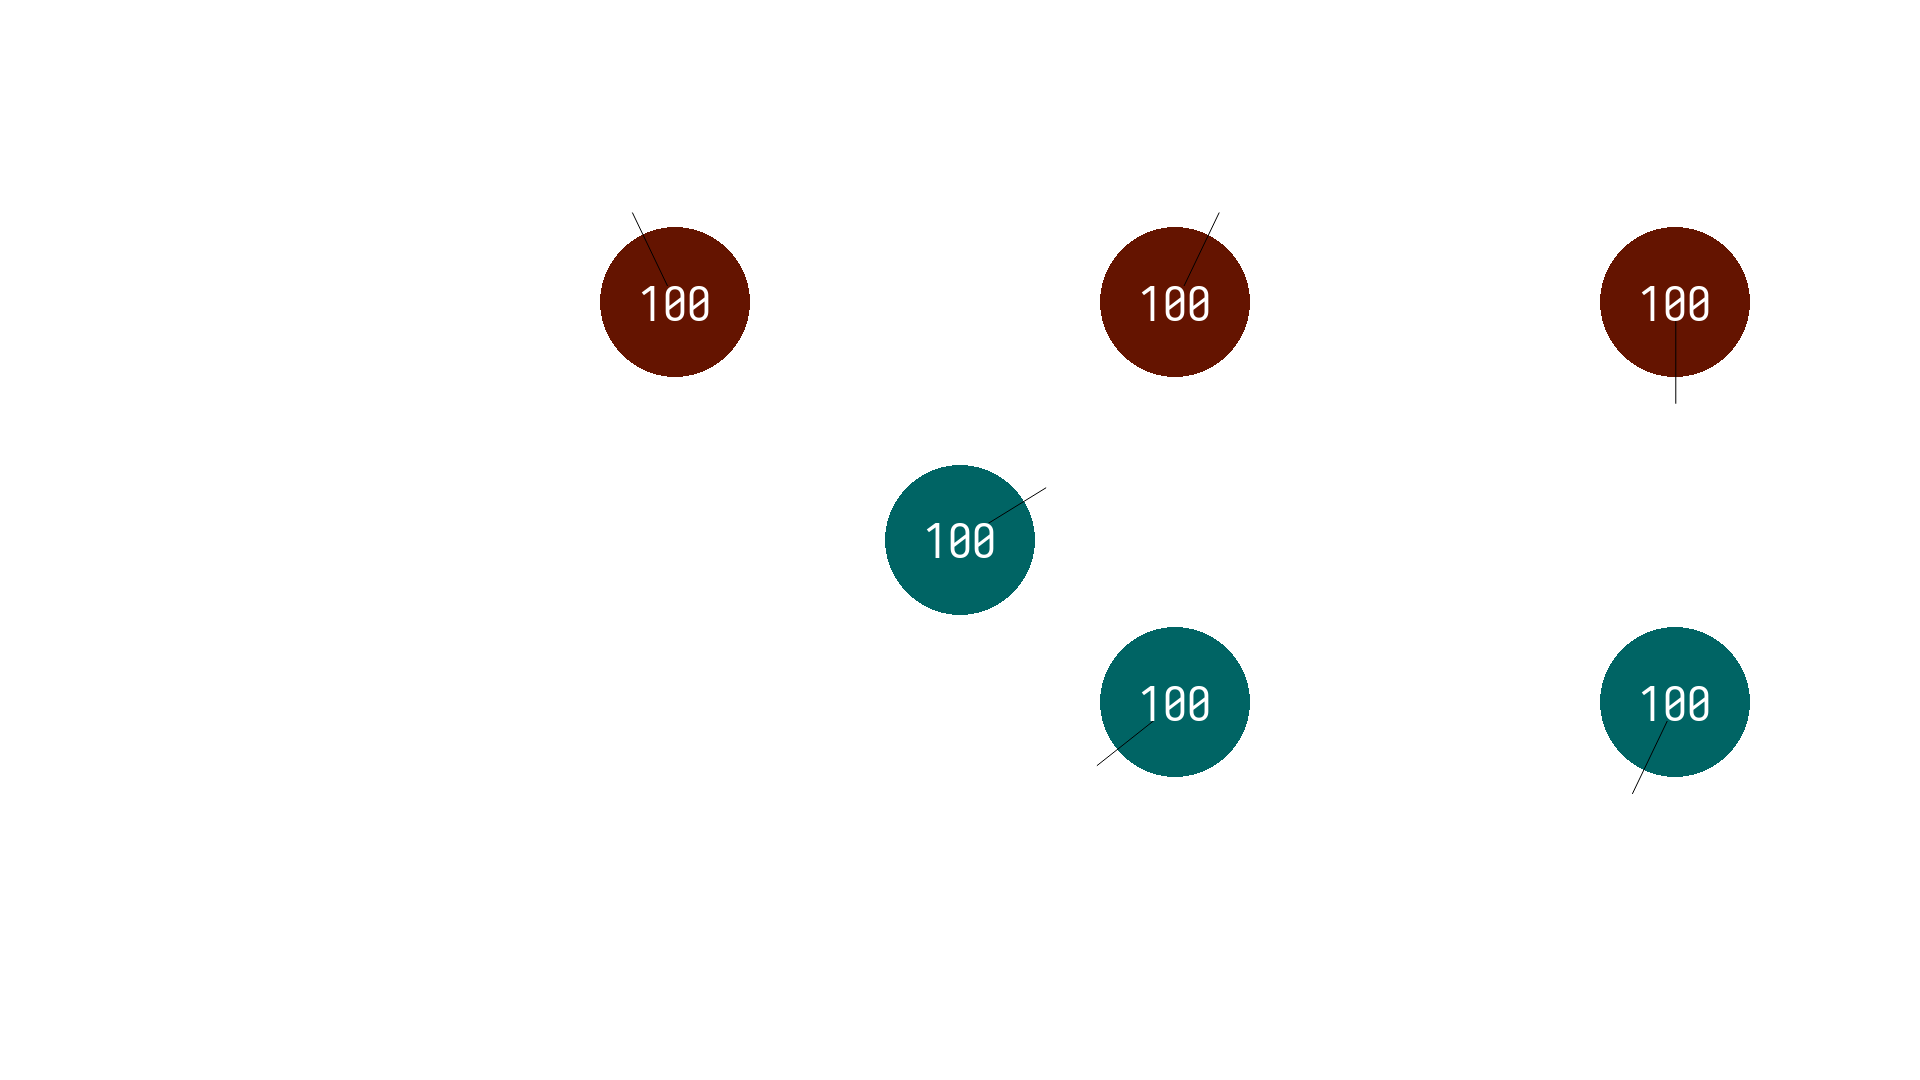
\includegraphics[width=\linewidth]{Development/Images/game_loop_4.png}}
    }
    \caption{A screen capture of the game loop with the health drawn on the players.}
    \label{fig:game_loop_4}
\end{figure}

We will now create \m{handleRayCollisions()} which takes in the \m{rays} dictionary containing all of the rays and which players were the source.

\begin{mpy}



\end{mpy}

\href{https://www.youtube.com/watch?v=VpSWuywFlC8}{Refer to this video since we will be doing collisions using rectangles not circle}

\href{https://gamedev.stackexchange.com/questions/199861/collision-detection-between-moving-objects-in-pygame}{This one might help too just take a look.}


\clearpage
\section{Development - Iteration 2}
\subsection{\textcolor{red}{Database Handling}}

Based on our previous discussion of using the \m{Utility} class through its static methods, we can also update the \m{DatabaseHandler} to use static methods too, which are more efficient in Python. This involves just removing the references to \m{self}.


\subsection{\textcolor{red}{Optimisation}}

One of the things that we will be improving in the project is optimisation. We need to be able to run many frames per second and therefore, we need to be able to optimise the code. In order to do this, we will use the package \m{Cython}. In order to do this, we will compile all of the classes that we have written in order to make them more efficient to prevent excessive recompilation.
\vs

To do this, we can create a \m{setup.py} file, and convert all of our files in to \m{.pyx} files. The setup file is as follows for each \m{.pyx} file that we want to use.

\begin{mpy}
import cython
from setuptools import setup

from Cython.Build import cythonize

setup(ext_modules = cythonize("utils.pyx"))
\end{mpy}

Running this code, we get some new files, namely \m{utils.c} and \m{utils.cp310-win_amd64.pyd}. This still functions exactly like a normal Python class however, and we still retain all of the functiosn that we had in the original class.

\tbc

\subsection{\textcolor{red}{Game Loop HUD}}

The Heads-up Display, will just be showing the score for each team, and the total amount of time left in the game. This will be done by tracking the amount of time that has passed in seconds, and then writing it to the screen using the button class we created. The score will be created using two more buttons on either side.

\vs
However, before that can happen we need to find a way of computing the score. To do that we will simply use a for loop. However, since one already exists in our code, we can use that but add another line to it.

\vs
\begin{mpy}
            #Render players as needed
            for i, player in enumerate(self.players, 0):
                player.render(self.display, self.player1.position, self.SCREEN_DIMS, zoom)

                self.scores[player.team] += deltaDamageCredit[player] + 50 * deltaEliminationCredit[player] - 50*deltaDeathCredit[player]

\end{mpy}

This can be done by adding text renders to the \m{GameLoop} class. We will create a new function. 

\begin{mpy}
    def drawHUD(self):
        #Find remaining time
        currentTime = time.time()
        if currentTime - self.startTime >= self.maxTime:
            return False

        timeRemaining = int(300 - (currentTime - self.startTime))

        minutesRemaining = timeRemaining // 60
        secondsRemaining = timeRemaining % 60

        #Render time text
        time_text_surface, time_text_rect = text_font.render(str(minutesRemaining) + ":" + str(secondsRemaining), 
            fgcolor=(255, 255, 255), bgcolor=(0, 0, 0))

        #Set position on the screen
        time_text_rect.center = [self.SCREEN_DIMS[0]//2, 50]

        #Draw background rectangle
        pygame.draw.rect(self.display, (0,0,0), self.time_rect)

        self.display.blit(time_text_surface, time_text_rect)

        #Scores for each team
        #Team 1
        score1_text_surface, score1_text_rect = text_font.render(str(self.scores[0]), 
            fgcolor=(255, 255, 255), bgcolor=(0, 0, 255))

        score1_text_rect.center = self.score_1_rect.center
        pygame.draw.rect(self.display, (0, 0, 255), self.score_1_rect)
        self.display.blit(score1_text_surface, score1_text_rect)

        #Team 2
        score2_text_surface, score2_text_rect = text_font.render(str(self.scores[1]), 
            fgcolor=(255, 255, 255), bgcolor=(255, 0, 0))

        score2_text_rect.center = self.score_2_rect.center
        pygame.draw.rect(self.display, (255, 0, 0), self.score_2_rect)
        self.display.blit(score2_text_surface, score2_text_rect)

        return True

\end{mpy}

This code will produce the following output. As you can the score updates based on the things that are happening within the game.


\begin{figure}[H]
        \centering
        {
        \setlength{\fboxsep}{0pt}%
        \setlength{\fboxrule}{1pt}%
        \fbox{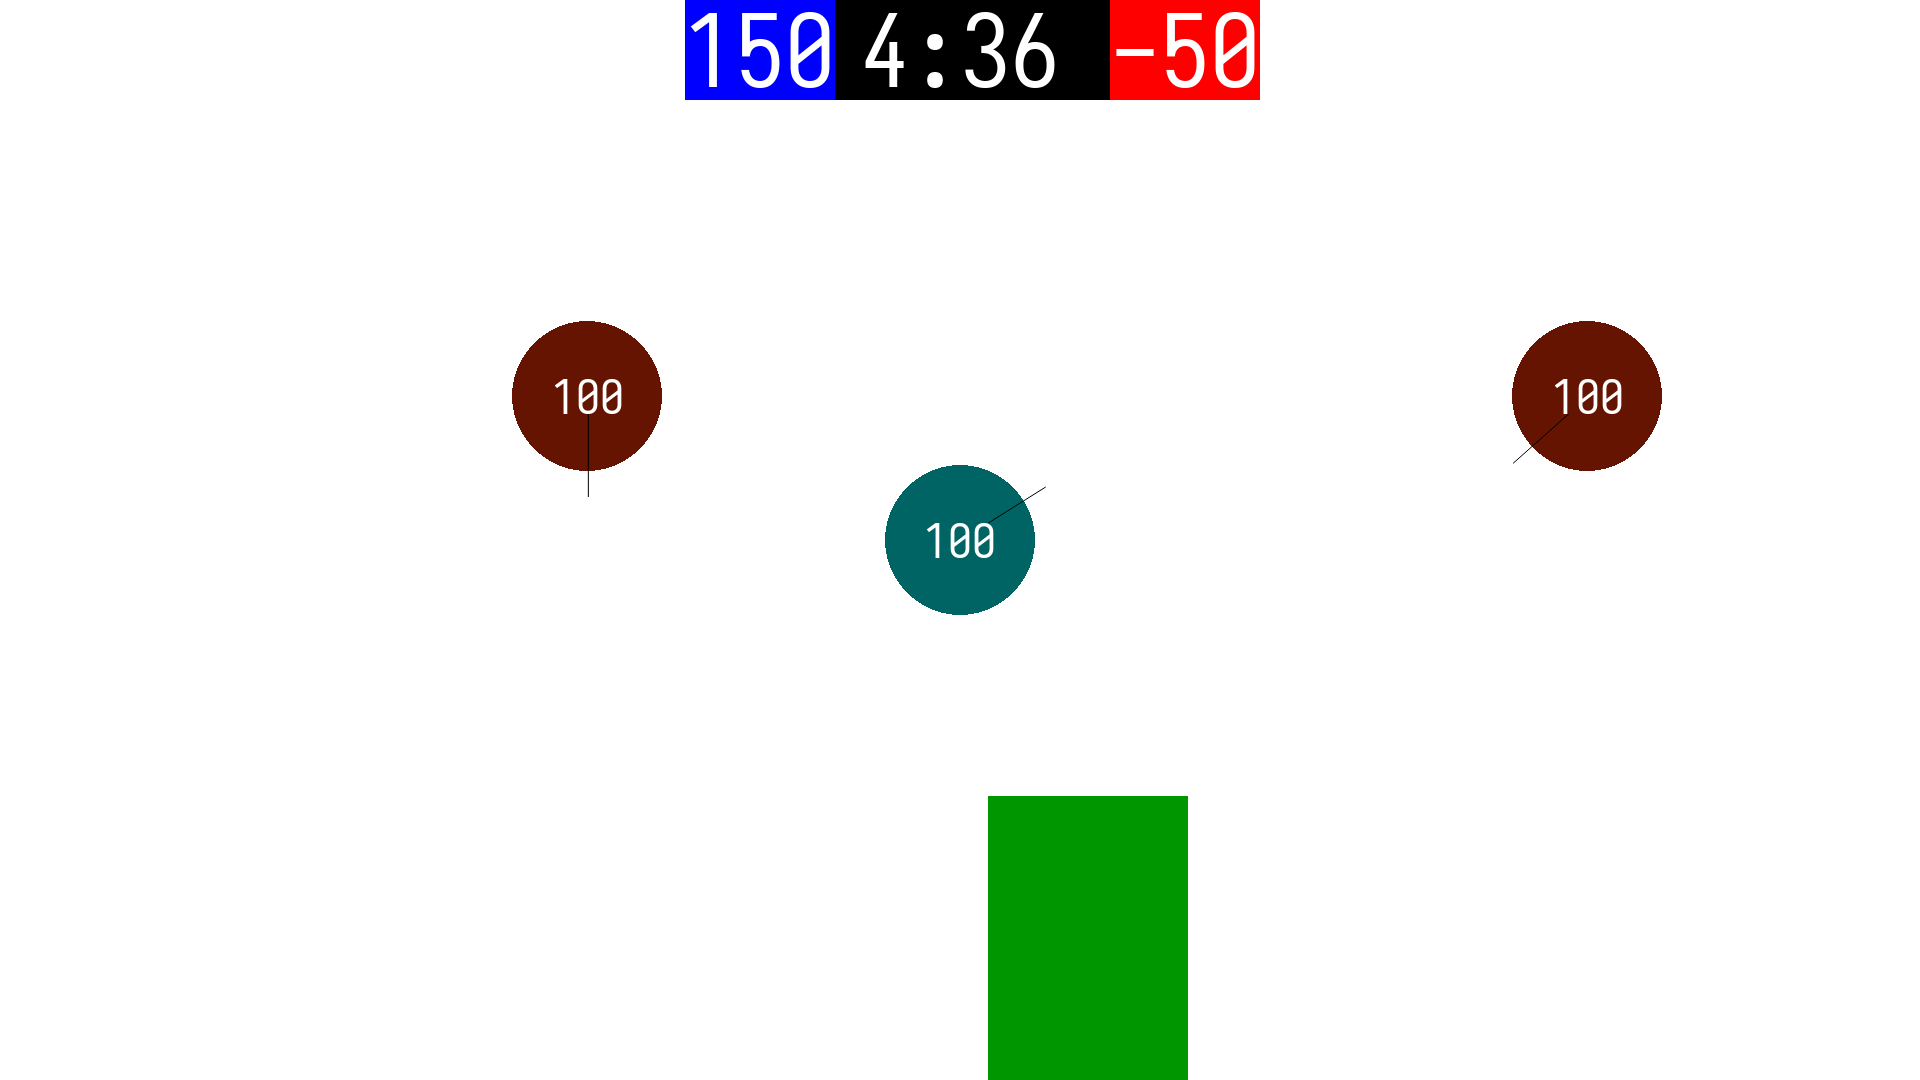
\includegraphics[width=\linewidth]{Development/Images/game_loop_2_1_hud.png}}
        }
        \caption{A screen capture of the map being zoomed out via the bound buttons}
        \label{fig:game_loop_2_1_hud}
\end{figure}

\vs
With this done, we can now return the total score for each team at the end of the game.


\subsection{\textcolor{red}{Environment}}

The first thing we need to do before starting doing any AI is to create the environment. This involves converting our game loop into something that can be run by a program which is then used to train the AI.

\vs
The first step in doing this is to remove all of the rendering functions. This is because we aren't rendering the game anymore and so we can just remove it. However, for the moment we will just create a copy of the game and comment out all of the rendering references in the main game loops. We only need the \m{GameLoop.run()} function primarily. 

\vs

Here I have imported all of the libaries that I need to run my training environment.

\begin{mpy}
from pettingzoo import ParallelEnv
from momentum_env.weapon import Weapon, Shotgun, AssaultRifle, SniperRifle
from momentum_env.player import Player
from momentum_env.block import Block
from momentum_env.utils import Utility as U
import numpy as np

import functools
from copy import copy

from gymnasium.spaces import Discrete, MultiBinary, Dict, Box, Tuple
from gymnasium.spaces.utils import flatten_space
from math import pi
\end{mpy}

Now, I need to create my environment's constructor. For this, I have just removed all of the calls to rendering and anything related to graphics. This has most of the same code as the constructor from the \m{GameLoop} class.

\begin{mpy}
class Momentum(ParallelEnv):
    metadata = {
        "name": "momentum_env",
    }

    def __init__(self, set_seed=42):
        self.REFRESH_RATE = 240
        self.dt = 1 / self.REFRESH_RATE

        # Team 1
        self.player1 = Player([1000, 3000], [0, -1], 0, Shotgun(self.REFRESH_RATE))
        self.player2 = Player([2000, 3000], [0, -1], 0, AssaultRifle(self.REFRESH_RATE)
        )
        self.player3 = Player([3000, 3000], [0, -1], 0, SniperRifle(self.REFRESH_RATE)
        )

        # Team 2
        self.player4 = Player([3000, 1000], [0, 1], 1, Shotgun(self.REFRESH_RATE))
        self.player5 = Player([2000, 1000], [0, 1], 1, AssaultRifle(self.REFRESH_RATE))
        self.player6 = Player([1000, 1000], [0, 1], 1, SniperRifle(self.REFRESH_RATE))

        # Contains all of the players in the game
        self.players = [self.player1, self.player2, self.player3, self.player4, self.player5, self.player6]

        #Blocks
        self.block1 = Block([1500, 2000], 200, 1200)
        self.block2 = Block([2500, 2000], 200, 1200)
        #self.block3 = Block([1000, 2000], 400, 400)
        #self.block4 = Block([2000, 2000], 400, 400)
        #self.block5 = Block([3000, 2000], 400, 400)

        #List of all blocks
        self.blocks = [self.block1, self.block2]#, self.block3, self.block4, self.block5]

        #Set countdowns
        self.countdowns = {p: 0 for p in self.players}
\end{mpy}

Furthermore, we want to be able to interchange between player instances and labels and so we will use dictionaries since they are perfect for this purpose. We will also create an array of all of the agents, so that the AI code can find the agents that we want to use.


\begin{mpy}
        #Access player object using string
        self.playerLabel = {"player1": self.player1,
                            "player2": self.player2,
                            "player3": self.player3,
                            "player4": self.player4,
                            "player5": self.player5,
                            "player6": self.player6,
        }

        #Access player string using player object
        self.invPlayerLabels = {self.player1: "player1",
                                self.player2: "player2",
                                self.player3: "player3",
                                self.player4: "player4",
                                self.player5: "player5",
                                self.player6: "player6",
        }

        #Player strings
        self.possible_agents = ["player1", "player2", "player3", "player4", "player5", "player6"]

        #Current timestep
        self.timesteps = 0

        self.agent_selection = copy(self.possible_agents)

        #Max timesteps in a game
        self.max_timestep = 6000

        self.scores = {0: 0, 
                       1: 0}

        self.max_score = 600

        self.agents = copy(self.possible_agents)
\end{mpy}


We need to create our observation and action spaces. This is done using the \m{gym} API, specifically the \m{Spaces} class, which will let us define th behaviour of our observation and action spaces.

\begin{mpy}

        low_obs = [0] * 8 + [0] * 8 + [-1]*8 + [0] + [0]
        high_obs = [1] * 8 + [100] * 8 + [1]*8 + [100] + [1]

        obs_space = Box(low=np.array(low_obs), high=np.array(high_obs), shape=(26,), dtype=np.float32)

        self.observation_spaces = {a: obs_space for a in self.agents}


        low_act = [-1, -1, -pi, 0]
        high_act = [1, 1, pi, 1]

        action_space = Box(low=np.array(low_act), high=np.array(high_act), shape=(4,), dtype=np.float32)

        self.action_spaces = {a: action_space for a in self.agents}


    #Nothing to really do here
    def set_seed(self, seed):
        pass

\end{mpy}

We will just copy the code for handling collisions from before. This has all already been tested, so we don't need to redo this step.

\begin{mpy}
    # Checks for hits between rays and objects in the map
    def handlePlayerCollisions(self):

        #Iterate through players
        for player in self.players:

            #Get player circle
            playerCircle = [player.position, player.radius]

            #Iterate through all possible collisions
            for collision_player in self.players:

                #Don't self-check
                if collision_player != player:

                    #Collision checking
                    hitResult = U.circleCircleCollision(playerCircle, [collision_player.position, collision_player.radius])

                    #If a collision happened
                    if hitResult[0] == True:

                        #Resolve it
                        player.position = U.vecAdd(player.position, hitResult[1])
                        collision_player = U.vecSub(collision_player.position, hitResult[1])

    #Collisions with the blocks
    def handleBlockCollisions(self):

        #Iterate through all players
        for player in self.players:

            #Iterate through all blocks
            for block in self.blocks:

                #Check for collision
                delta = U.circleRectCollision(player, block)

                #Resolve
                if delta[0]:
                    player.position = U.vecAdd(player.position, delta[1])

    def handleRayCollisions(self, rays):
        
        #Dicts for credit
        damageCredit = {p: 0 for p in self.players}
        eliminationCredit = {p: 0 for p in self.players}
        deathCredit = {p: 0 for p in self.players}

        #Iterate through all players
        for player_i in self.players:
            firedRays = rays[player_i]

            for ray in firedRays:

                #Larger than possible hit range
                t = 2
                bestHit = None
                
                #Line we want to test with
                line = ray[0:2]

                #Iterate through all blocks
                for block in self.blocks:

                    #Determine whether a result is met
                    hitResult = U.lineRectCollision(line, block)

                    #If a hit has occurred
                    if hitResult[0]:

                        #If the result is closer
                        if hitResult[1] < t:

                            #Reassign the hit result
                            t = hitResult[1]


                #Iterate through test players
                for testPlayer in self.players:

                    #Don't check if test is the player
                    if testPlayer != player_i and testPlayer.team != player_i.team:

                        #Player circle
                        circle = [testPlayer.position, testPlayer.radius]

                        #Check if hit has occurred
                        hitResult = U.lineCircleCollision(line, circle)

                        #Is there a hit, and was it closer
                        if hitResult[0] and t > hitResult[1]:

                            #If so, update bestHit and min t
                            t = hitResult[1]
                            bestHit = testPlayer

                #If hit registered
                if bestHit:

                    #Reduce health of player which was killed
                    bestHit.health -= ray[2]
                    
                    #If player died
                    if bestHit.health <= 0:

                        #Reset the player
                        bestHit.reset()

                        #Add elim credit to player_i
                        eliminationCredit[player_i] += 1

                        #Add death credit to player which died
                        deathCredit[bestHit] += 1

                    #Add damage credit to player_i for the hit
                    damageCredit[player_i] += ray[2]


        return damageCredit, eliminationCredit, deathCredit
\end{mpy}

Next, we will get the observations for each player. This is code that we will need to be added to the main environment as well.

\vs
We need to decide what observations we want to feed to the agents and in what format. There will be 16 spokes, which will be equally spread out angularly across the player's field of vision. These will then intersect with other players and blocks. We will return the ratio of the distance from the end of the spoke to the intersection and the length of the spoke. We also want to return the type of the intersection. For each spoke we can have 3 things happening.

\begin{enumerate}[label=\arabic*.]
    \item Nothing happens, there are no intersections.
    \item A player or enemy is standing somewhere along the spoke.
    \item There is a block intersecting with the spoke.
\end{enumerate}

We want to handle these accordingly.

\begin{enumerate}[label=\arabic*.]
    \item We want to return a 0 for the distance and a 0 for the intersection type
    \item We want to return the ratio of the intersection distance and the length of the spoke, and a 1 or -1 multiplied by the player health for the intersection type depending on whether the player is a team-mate or enemy
    \item We want to return the ratio of the intersection distance and the length of the spoke, and 0 for the intersection type
\end{enumerate}

The actual order of the inputs does not matter since we are using a neural network, as long as it is consistent. There are some additional inputs we need to add. The first one is for what angle the player is at with respect to their initial forward vector. We can find this using the dot product, or we can track it directly. Using the dot product will give a much more consistent answer however.

\vs
On top of this we want to give other inputs showing whether we can fire or not in any given frame, and if not how long we have until we can. Furthermore, we want to give the health of the agent as an input so it can make more responsible choices.

\begin{mpy}
    def getObservations(self, player):

        spokes = player.detectionSpokes()

        distances = []
        healths = []
        alliances = []

        for spoke in spokes:


            #Larger than possible hit range
            t = 2
            bestHit = None
            
            #Line we want to test with
            line = spoke

            #Block hit
            blockHit = False


            #Iterate through all blocks
            for block in self.blocks:

                #Determine whether a result is met
                hitResult = U.lineRectCollision(line, block)

                #If a hit has occurred
                if hitResult[0]:

                    #If the result is closer
                    if hitResult[1] < t:

                        #Reassign the hit result
                        t = hitResult[1]
                        blockHit = True


            #Iterate through test players
            for testPlayer in self.players:

                #Don't check if test is the player
                if testPlayer != player:

                    #Player circle
                    circle = [testPlayer.position, testPlayer.radius]

                    #Check if hit has occurred
                    hitResult = U.lineCircleCollision(line, circle)

                    #Is there a hit, and was it closer
                    if hitResult[0] and t > hitResult[1]:

                        #If so, update bestHit and min t
                        t = hitResult[1]
                        bestHit = testPlayer
                        blockHit = False
                            
            #Case 1
            if not blockHit and not bestHit:
                distances.append(0)
                healths.append(0)
                alliances.append(0)

            #Case 2
            if not blockHit and bestHit:
                if bestHit.team == player.team:
                    team = 1
                else:
                    team = -1
                distances.append(1-t)
                healths.append(bestHit.health)
                alliances.append(team)

            #Case 3
            if blockHit and not bestHit:
                distances.append(1-t)
                healths.append(0)
                alliances.append(0)

        #Add player information
        #Add player health
        #Add whether player is on cooldown or not

        countdown = self.countdowns[player]
        if countdown <= 0:
            can_fire = True
        else:
            can_fire = False

        observations = distances + healths + alliances
        observations.append(player.health)
        observations.append(can_fire)

        #obs = {self.invPlayerLabels[player]: observations, 'mask': [True, True, True, True]}

        return observations
\end{mpy}


We also need to add a function for resetting the environment, which is done by setting the environment back to it's original environment.

\begin{mpy}
    def reset(self, seed=None, options=None):

        self.agents = copy(self.possible_agents)

        for player in self.players:
            player.reset()

        #Reset countdowns
        self.countdowns = {p: 0 for p in self.players}

        self.timestep = 0

        infos = {a: {} for a in self.agents}

        observations = {a: self.getObservations(self.playerLabel[a]) for a in self.agents}

        rewards = {a: 0 for a in self.agents}
        terminations = {a: False for a in self.agents}
        truncations = {a: False for a in self.agents}
        
        self.lastVals = observations, rewards, terminations, truncations, infos

        return observations, infos
\end{mpy}

We also have added a step function for taking an action from the agents and then updating the state, returning new observations and rewards from this environment.

\begin{mpy}
    def step(self, actions):

        rays = {}

        #Update player states
        for i, player in enumerate(self.players, 0):

            playerStringLabel = self.invPlayerLabels[player]
            playerActions = actions[playerStringLabel]

            action = {"forward": playerActions[1],
                    "right": playerActions[2],
                    "rot_rate": playerActions[3],
                    "firing": playerActions[0]}

            rays[player], fired = player.updatePlayerState(action, self.countdowns[player], self.dt)

            if fired:
                self.countdowns[player] = player.weapon.maxFrameCooldown
            else:
                self.countdowns[player] -= 1

        #Handle collision
        self.handlePlayerCollisions()
        self.handleBlockCollisions()
        
        #Handle ray collisions
        deltaDamageCredit, deltaEliminationCredit, deltaDeathCredit = self.handleRayCollisions(rays)        
        

        #Create rews
        rewards = {a: 0 for a in self.agents}

        #Attribute rewards
        for player in self.players:
            rew = deltaDamageCredit[player] + deltaEliminationCredit[player] * 75 - 75 * deltaDeathCredit[player] + (abs(1500 - player.position[0]) + abs(1500 - player.position[1]))/250
            a = self.invPlayerLabels[player]
            rewards[a] = rew

        #Adjust score
        for player in self.players:
            deltaScore = deltaDamageCredit[player] + deltaEliminationCredit[player] * 75
            self.scores[player.team] += deltaScore

        #Truncation conditions
        truncations = {a: False for a in self.agents}
        if self.timesteps > self.max_timestep:
            truncations = {a: True for a in self.agents}

        #Termination condition
        terminations = {a: False for a in self.agents}
        for i in range(0, 2):
            if self.scores[i] > self.max_score:
                for player in self.players:
                    a = self.invPlayerLabels[player]
                    if player.team == i:
                        rewards[a] += 200
                    else:
                        rewards[a] -= 100

        #Get observations
        observations = {a: self.getObservations(self.playerLabel[a]) for a in self.agents}

        #Additional info - dummy
        infos = {a: {} for a in self.agents}

        #If terminated
        if any(terminations.values()) or all(truncations.values()):
            self.agents = []

        #Increment timestep
        self.timestep += 1

        self.lastVals = observations, rewards, terminations, truncations, infos

        return observations, rewards, terminations, truncations, infos
\end{mpy}

Finally, we have some extra functions that we need to set, but these are fairly self-explanatory.

\begin{mpy}
    def render(self):
        pass

    def observation_space(self, agent):
        return self.observation_spaces[agent]

    def action_space(self, agent):
        return self.action_spaces[agent]

    def last(self, something):
        return self.lastVals
\end{mpy}


\subsection{\textcolor{red}{Training and AI}}

We will be using the standard implementation of PPO in the official PyTorchRL tutorials and documentation. We will modify this in order to use this in a IPPO context. Another change compared to the rest of this project is that we will be using Jupyter Notebooks for the AI training. This is because it is much more convenient that using a Python script, since we can re-run small sections of the code without having to re-run the entire script. This is useful since Python is an interpreted language, and AI scripts can take a very long time to run, and so if there is some problem later on in the program, we could potentially lose a lot of progress. However, using these Notebooks means that we can add code blocks on to the end and can re-run them if errors happen.

\vs

We will first need to import all of the relevant libraries and modules that we need to write and run the code. This is primarily \m{torch} and \m{torchrl} modules in order to write the neural networks and creating a replay buffer, which is essential to the training process. We effectively rollout the policy for a number of timesteps, and then we update the model using the recorded trajectories from the rollout. To do this, we use something that \m{torchrl} uses makes extensive use of which is the \m{TensorDict} library. This will let us use dictionaries of tensors which are the primary objects which neural networks work with.

\vs
In order to speed up the training process, we will be using the GPU. This will let us conduct many tensor operations in parallel much more effectively. We can do this as follows.

\begin{mpy}
>>> print(torch.cuda.is_available())
True
>>> device = torch.device(0)
>>> print(device)
cuda:0
\end{mpy}

\vs
This confirms that we have indeed used the GPU. We will use this in all of our scripts in order to ensure that we have efficient code execution and improve performance. It also means that if there is a problem in the model when running it initially, we will not be too far behind and can retrain relatively easily.
\vs

The very first thing to do is to import all of the libraries that we need in order to train our agent. This is done as follows.

\begin{mpy}
#Torch
import torch
from tensordict.nn import TensorDictModule, TensorDictSequential
from tensordict.nn.distributions import NormalParamExtractor
from torch import nn

#Data
from torchrl.collectors import SyncDataCollector
from torchrl.data.replay_buffers import ReplayBuffer, TensorDictReplayBuffer, LazyTensorStorage, SamplerWithoutReplacement

#Modules
from torchrl.modules import ProbabilisticActor, ValueOperator, TanhNormal, MultiAgentMLP

#Objectives
from torchrl.objectives import ClipPPOLoss, ValueEstimators
from torchrl.objectives.value import GAE

#Multi-processing
from torch import multiprocessing
from torchrl.envs import RewardSum, TransformedEnv, check_env_specs, Transform

#Envs
from momentum_env.momentum_env import Momentum
from torchrl.envs import PettingZooWrapper
\end{mpy}

Now, that we our libraries imported, we will now create the instance of our environment.

\begin{mpy}
env = Momentum()
group_map = {"team0": ['player1', 'player2', 'player3'],
            "team1": ['player4', 'player5', 'player6']}

env = PettingZooWrapper(env, group_map=group_map)
\end{mpy}

We will now define our hyperparameters which will be used to train our networks.

\begin{mpy}
device = torch.device("cpu")

# Sampling
frames_per_batch = 6_000  # Number of team frames collected per training iteration
n_iters = 30  # Number of sampling and training iterations
total_frames = frames_per_batch * n_iters

# Training
num_epochs = 10  # Number of optimization steps per training iteration
minibatch_size = 100  # Size of the mini-batches in each optimization step
lr = 3e-4  # Learning rate
max_grad_norm = 1.0  # Maximum norm for the gradients

# PPO
clip_epsilon = 0.2  # clip value for PPO loss
gamma = 0.9  # discount factor
lmbda = 0.9  # lambda for generalised advantage estimation
entropy_eps = 1e-4
\end{mpy}

Now that we have our environment and hyperparameters, we will define our actor and critic networks. However, the way that PPO trains the model is to use multi-variate normal distributions. This is because this allows for a certain amount of randomness when training and this means that we can explore the environment more and potentially uncover better policies to play the game by than the current one. So therefore, we will create two constructs, the first one being the actual model, and the other being the actor which we will use for the training. In this case, our policy network, will give the outputs of all of the agents of our team.

\vs
The next thing to do is to create a \m{Sequential} network which will take the observation in and will out a \m{loc} and \m{scale} for each value in each agent's action space.

\begin{mpy}
team0_policy_net = torch.nn.Sequential(
    MultiAgentMLP(
        n_agent_inputs=env.observation_spec["team0", "observation"].shape[-1],
        n_agent_outputs = 2 * 4,
        n_agents = 3,
        centralised = False,
        share_params = False,
        device=device,
        depth=2,
        num_cells = 128,
        activation_class = torch.nn.Tanh,
    ),
    NormalParamExtractor(),
).to(device)

\end{mpy}

The number of agents on each team is 3, and therefore this policy will act on behalf of all three agents. We will now create a \m{TensorDictModule} which will let \m{TorchRL} more easily track the values that we are using, and means that we can much more easily debug the code. Using keys in this regard means that the behaviour of the code is much more easily understandable and controllable.

\begin{mpy}
team0_policy_module = TensorDictModule(
    team0_policy_net,
    in_keys = [("team0", "observation")],
    out_keys = [("team0", "loc"), ("team0", "scale")],
).to(device)
\end{mpy}

Finally, we want to wrap this in a \m{ProbabilisticActor}. This will mean that the \m{loc} and \m{scale} that we produced earlier will now be used in a \m{TanhNormal} distribution (a combination of a $\tanh$ distribution and a normal distribution). This will produce a final action for the team.

\vs
Now, we want to replicate all of this but now for the second team. This is so that we can get two 


\subsection{\textcolor{red}{Game Loop}}


\vs
We have a few more changes to make before we can finalise the game. Firstly, we need to find a way to find the score of each player. This is different to the reward function, but still needs to be done. Primarily, we want to credit for damage dealt and any eliminations in the whole game, and penalise for any deaths. This is appears as following in the code. We can do this for each frame, but we need to have a dictionary handling this for every player in the map. We only need to do this at the end of the game loop, since the score won't be visible to the player during the round anyway.

\begin{mpy}



\end{mpy}

We also need to set an objective for the game and whether the game has ended or not. The main objective will be either eliminations or team score, and the game can end if the objective is met or if the timer has run out. We can do this follows. The score, the damage dealt, the eliminations and the deaths will all be passed to the game over menu, which will then be able to render everything. We want to display the user's score and how they performed against the enemy team. We can track the game length using frames once more. We can find the total lengths of the games in frames by tracking the numbers of second the game should last and the frame rate.

\begin{mpy}


\end{mpy}

Now that the values have been returned we can decompose them and render the text to the screen. The code for the game over menu appears as follows.


\begin{mpy}



\end{mpy}


We can write the time left and the team scores on the screen whilst the game is running. We will set the round time to be short so that we can observe the game ending due to running out of time. We will be using the button class once more to write text to the screen and just update the text on the \m{Button} every tick.

\begin{mpy}


\end{mpy}

{\huge \textcolor{red}{INSERT FIGURE AND VIDEO HERE}}

\clearpage
\section{Evaluation}
\subsection{\textcolor{red}{Usability Testing}}

\tbc

\subsection{\textcolor{red}{Reviewing Success Criteria}}

\tbc

\subsection{\textcolor{red}{Un-met Criteria}}

\tbc

\subsection{\textcolor{red}{Usability Features}}

\tbc

\subsection{\textcolor{red}{Further Development}}

\tbc

\subsection{\textcolor{red}{Maintenance Issues}}

\tbc

\subsection{\textcolor{red}{Limitations of the Solution}}

\tbc

\subsection{\textcolor{red}{Developments on Limitations}}

\tbc

%\clearpage
%\section{\textcolor{red}{To-Do List}}
%\subsection{Subsections}

\begin{center}
\begin{longtable}{|p{3.5cm}|p{10cm}|}
    \hline
    Section & Subsections\\
    \hline
    \hline
    Analysis & \begin{itemize}
        \item Problem Definition
        \item Analysis of Existing Solutions
        \item Explanation of Choice of Project
        \item Stakeholders
        \item Interviews
        \item Analysis of Interviews
        \item Essential Features
        \item Stakeholder and Public Requirements Summary
        \item Justification of Computational Methods
        \item Limitations of Proposed Solution
        \item Success Criteria
    \end{itemize}\\
    \hline
    Design & \begin{itemize}
        \item Game States
        \item Game Loop
        \item Movement
        \item Weapons
        \item Database Management
        \item UI
        \item AI / Training Environment
        \item Utility Class
    \end{itemize}\\
    \hline
    Development - Iteration 1 & \begin{itemize}
        \item Main
        \item Game State Manager
        \item Player
        \item Menus
        \item Database Handling
        \item Weapon
        \item Game Loop
        \item Utilities
    \end{itemize}\\
    \hline
    Development - Iteration 2 & \begin{itemize}
        \item Game Loop Adjustments
        \item Render Functions
        \item Database Changes (static methods)
        \item Environment Adjustments
        \item AI Agent / Training
        \item Menus
    \end{itemize}\\
    \hline
    Testing & \begin{itemize}
        \item Game State Manager
        \item Player
        \item Menus
        \item Database Handling
        \item Weapon
        \item Game Loop
        \item Utilities
        \item Rendering
        \item AI Testing
    \end{itemize}\\
    \hline
    Evaluation & \begin{itemize}
        \item Annotated Evidence for usability testing
        \item Cross-reference with success criteria
        \item Comments on um-met criteria
        \item Evidence of usability features
        \item Ideas for further development
        \item Maintenance issues
        \item Limitations of the solution
        \item Developments to deal with limitations
    \end{itemize}\\
    \hline
\end{longtable}
\end{center}

\clearpage
\subsection{Actions}

\begin{center}
\begin{longtable}{|p{7cm}|p{2.5cm}|p{4cm}|}
    \hline
    Action & Started? & Time to Completion\\
    \hline
    \hline
    Essential Features & No & 30 minutes\\
    \hline
    Analysis of Interviews & No & 30 minutes\\
    \hline
    More Success Criteria & No & 30 minutes\\
    \hline
    Game States Table & Yes & 15 minutes\\
    \hline
    Game Loop Table & Yes & 5 minutes\\
    \hline
    Movement Review & No & 15 minutes\\
    \hline
    Weapons & No & 45 minutes\\
    \hline
    Database review & No & 15 minutes\\
    \hline
    UI & No & 30 minutes\\
    \hline
    AI Review & No & 15 minutes\\
    \hline
    Utility Class & No & 30 minutes\\
    \hline
\end{longtable}
\end{center}

\clearpage
\subsection{Overall Aims}

\begin{center}
\begin{longtable}{|p{8cm}|p{2.5cm}|p{3.8cm}|}
    \hline
    Task & Started? & Time To Completion\\
    \hline
    \hline
    Annotated Diagrams of the other games & Done & -\\
    \hline
    Analysis of interviews & No & 1 hour\\
    \hline
    Subheadings for justification in every section & No & 1 hour\\
    \hline
    Grid for limitations, with one column for requirement, justification, the limitation itself (why we can't do this thing) & No & 1 hour\\
    \hline
    Success Criteria Table (Number, Requirements, Justification, Done, Reference) & Yes & 30 minutes\\
    \hline
    Big systems diagram, colour coded & Yes & 1 hour\\
    \hline 
    Explain how stakeholders will make use of the proposed solution & No & 1 hour\\
    \hline
    Explanation of each module in the design and seperate justification headings & No & 1 hour\\
    \hline
    Usability Features & No & 1 hour\\
    \hline
    Class Diagrams & No & 1 hour\\
    \hline 
    Flowcharts for each small section in the design & No & 2 hours\\
    \hline
    Key Variables and Data Structures in a big table and explain and justify them & No & 2 hours\\
    \hline 
    Justification of Computational Methods - Separate it into headings & Yes & 1 hour\\
    \hline
    Add a section in the analysis for the features of the computational solution & No & 1 hour\\
    \hline
    Limitations need to be justified & No & 1 hour\\
    \hline
    Acceptance Testing & No & N/A\\
    \hline
    Put dates into the development timeline for major changes & No & N/A\\
    \hline
    Be honest and document if you don't know how to do something fully & Yes & N/A\\
    \hline
    Reference the original tutorials & No & N/A\\
    \hline
\end{longtable}
\end{center}

\clearpage
\subsection{Development Checklist}

\begin{center}
\begin{longtable}{|p{2.5cm}|p{3.5cm}|p{4.8cm}|p{2.7cm}|}
    \hline
    File & Class & Method & Documented?\\
    \hline
    \hline
    \mintinline{py}{block.py} & \mintinline{py}{Block} & \mintinline{py}{__init__(self)} & No\\
    & & \mintinline{py}{render()} & No\\
    & & \mintinline{py}{getCorners()} & Yes\\
    \hline
    \hline
    \mintinline{py}{database.py} & \mintinline{py}{DatabaseHandler} & \mintinline{py}{SetupConnection()} & No\\
    & & \mintinline{py}{CloseConnection()} & No\\
    & & \mintinline{py}{CreateAccount()} & No\\
    & & \mintinline{py}{UpdateAccount()} & No\\
    & & \mintinline{py}{AuthenticateAccount()} & No\\
    \hline
    \hline
    \mintinline{py}{game.py} & \mintinline{py}{Game} &\mintinline{py}{__init__(self)} & No\\
    & & \mintinline{py}{run()} & No\\
    \hline
    & \mintinline{py}{GameLoop} & \mintinline{py}{__init__(self)} & No\\
    & & \mintinline{py}{checkHit()} & No\\
    & & \mintinline{py}{run()} & No\\
    \hline
    \hline
    \mintinline{py}{main.py} & - & - & No\\
    \hline
    \hline
    \mintinline{py}{player.py} & \mintinline{py}{Player} & \mintinline{py}{__init__(self)} & No\\
    & & \mintinline{py}{movePlayer()} & Yes\\
    & & \mintinline{py}{dash()} & No\\
    & & \mintinline{py}{fire()} & No\\
    & & \mintinline{py}{updatePlayerState()} & No\\
    & & \mintinline{py}{render()} & No\\
    \hline
    \hline
    \mintinline{py}{utils.py} & \mintinline{py}{Utility} & \mintinline{py}{dot()} & Yes\\
    & & \mintinline{py}{vecSub()} & Yes\\
    & & \mintinline{py}{vecAdd()} & Yes\\
    & & \mintinline{py}{mult()} & No\\
    & & \mintinline{py}{lineLineCollision()} & Yes\\
    & & \mintinline{py}{lineRectCollision()} & Yes\\
    & & \mintinline{py}{lineCircleCollision()} & Yes\\
    & & \mintinline{py}{circleRectCollision()} & No\\
    & & \mintinline{py}{circleCircleCollision()} & No\\
    & & \mintinline{py}{checkCircleInRange()} & No\\
    & & \mintinline{py}{checkBlockInRange()} & No\\
    & & \mintinline{py}{rotateVector()} & No\\
    & & \mintinline{py}{convertToScreen()} & No\\
    \hline
    \hline
    \mintinline{py}{weapon.py} & \mintinline{py}{Weapon} & \mintinline{py}{__init__(self)} & No\\
    & & \mintinline{py}{fire()} & No\\
    \hline
    & \mintinline{py}{AssaultRifle} & \mintinline{py}{__init__(self)} & No\\
    \hline
    & \mintinline{py}{SniperRifle} & \mintinline{py}{__init__self()} & No\\
    \hline
    & \mintinline{py}{Shotgun} & \mintinline{py}{__init__self()} & No\\
    \hline
    \hline
    \mintinline{py}{menu.py} & \mintinline{py}{GameStateManager} & \mintinline{py}{__init__(self)} & No\\
    & & \mintinline{py}{getState()} & No\\
    & & \mintinline{py}{setState()} & No\\
    \hline
\end{longtable}
\end{center}


The menu classes have been omitted from here, will be documented when there is more code there.

%\clearpage
%\section{Links To Follow}
%\href{https://gamedevacademy.org/pygame-menu-tutorial-complete-guide/}{Pygame Tutorial}

\vspace{11pt}
\href{https://pygame-menu.readthedocs.io/en/4.2.8/index.html}{Pygame-Menu Docs}

\vspace{11pt}
\href{https://www.youtube.com/watch?v=2iyx8_elcYg}{Menu System}

\vspace{11pt}
\href{https://www.youtube.com/watch?v=0RryiSjpJn0}{Menu System}

\vspace{11pt}
\href{https://www.youtube.com/watch?v=r0ixaTQxsUI}{Game States}


\vspace{11pt}
\href{https://www.youtube.com/watch?v=GMBqjxcKogA}{Menu System V2}

\vspace{11pt}
\href{https://towardsdatascience.com/training-an-agent-to-master-tic-tac-toe-through-self-play-72038c3f33f7}{Self-Play example}

\vspace{11pt}
\href{https://huggingface.co/learn/deep-rl-course/unit7/self-play}{Hugging Face Self-Play}

\vspace{11pt}
\href{https://github.com/younggyoseo/pytorch-nfsp}{Imperfect Information}

\vspace{11pt}
\href{https://openai.com/research/openai-baselines-ppo}{PPO}

\vspace{11pt}
\href{https://blog.unity.com/engine-platform/training-intelligent-adversaries-using-self-play-with-ml-agents}{Self-play history}

\vspace{11pt}
\href{https://openai.com/research/competitive-self-play}{Comp self-play}

\vspace{11pt}
\href{https://medium.com/applied-data-science/how-to-build-your-own-alphazero-ai-using-python-and-keras-7f664945c188}{Self-play keras}

\vspace{11pt}
\href{https://github.com/HarrisSteven/RL-Game/blob/master/Melee_Notebook.ipynb}{Melee Keras}

\vspace{11pt}
\href{https://modelzoo.co/model/chess-reinforcement-learning}{Chess}

\vspace{11pt}
\href{https://github.com/oxwhirl/pymarl}{PyMARL}

\vspace{11pt}
\href{https://ai.stackexchange.com/questions/26806/how-do-i-get-started-with-multi-agent-reinforcement-learning}{MARL}

\vspace{11pt}
\href{https://ai.stackexchange.com/questions/31627/multi-agent-deep-reinforcement-learning-for-continuous-and-discrete-action}{Continuous MARL}

\vspace{11pt}
\href{https://applied-rl-course.netlify.app/en/module2}{RL Lib}

\vspace{11pt}
\href{https://github.com/Farama-Foundation/PettingZoo}{Petting Zoo}

\vspace{11pt}
\href{https://rlss.inria.fr/files/2019/07/RLSS_Multiagent.pdf}{MARL Terms}

\vspace{11pt}
\href{https://github.com/DLR-RM/stable-baselines3}{Stable Baselines - Pytorch}

\vspace{11pt}
\href{https://github.com/DLR-RM/rl-baselines3-zoo}{Stable Baselines envs}

\vspace{11pt}
\href{https://karpathy.github.io/2016/05/31/rl/}{RL Basics}

\vspace{11pt}
\href{https://towardsdatascience.com/ultimate-guide-for-reinforced-learning-part-1-creating-a-game-956f1f2b0a91}{AI for PyGame}

\vspace{11pt}
\href{https://web.stanford.edu/~surag/posts/alphazero.html}{Alpha Zero}

\vspace{11pt}
\href{https://github.com/lucas-emery/rocket-league-gym}{Multi agents Rocket League}

\vspace{11pt}
\href{https://stable-baselines.readthedocs.io/en/master/guide/rl_tips.html}{RL Tips}

\vspace{11pt}
\href{https://stable-baselines3.readthedocs.io/en/master/search.html?q=multi+agent&check_keywords=yes&area=default#}{Stable Baselines MARL}

\vspace{11pt}
\href{https://pettingzoo.farama.org/environments/mpe/}{Particles}

\vspace{11pt}
\href{https://pettingzoo.farama.org/environments/atari/foozpong/}{Foozpong}

\vspace{11pt}
\href{https://pettingzoo.farama.org/environments/atari/quadrapong/}{Quadrapong}

\vspace{11pt}
\href{https://pettingzoo.farama.org/environments/butterfly/pistonball/}{Pistonball}

\vspace{11pt}
\href{https://pettingzoo.farama.org/environments/mpe/simple_tag/}{Tag}

\vspace{11pt}
\href{https://pettingzoo.farama.org/environments/sisl/multiwalker/}{Multiwalker}

\vspace{11pt}
\href{https://pettingzoo.farama.org/environments/sisl/waterworld/}{Waterworld}

\vspace{11pt}
\href{https://pettingzoo.farama.org/tutorials/sb3/kaz/}{Stable Baselines MARL PPO}

\vspace{11pt}
\href{https://pettingzoo.farama.org/tutorials/sb3/waterworld/}{Waterworld SB3 MARL PPO}

\vspace{11pt}
\href{https://docs.ray.io/en/latest/rllib/rllib-algorithms.html}{Multi RL Algos}

\vspace{11pt}
\href{https://github.com/philtabor/Youtube-Code-Repository/tree/master/ReinforcementLearning/PolicyGradient/PPO/tf2}{PPO TF2}

\vspace{11pt}
\href{https://github.com/philtabor/Youtube-Code-Repository/blob/master/ReinforcementLearning/PolicyGradient/PPO/torch/ppo_torch.py}{PPO Torch}

\vspace{11pt}
\href{https://pytorch.org/rl/reference/generated/torchrl.objectives.PPOLoss.html}{PPO Loss}

\vspace{11pt}
\href{https://github.com/abhisheksuran/Reinforcement_Learning/blob/master/PPO.ipynb}{TF2 PPO Code}


\section{Code Listings}

\subsection{main.py}

\inputminted[breaklines, tabsize=2, fontsize=\footnotesize]{py}{Code/main.py}

\clearpage

\subsection{block.py}

\inputminted[breaklines, tabsize=2, fontsize=\footnotesize]{py}{Code/block.py}


\clearpage


\subsection{game.py}

\inputminted[breaklines, tabsize=2, fontsize=\footnotesize]{py}{Code/game.py}


\clearpage


\subsection{player.py}

\inputminted[breaklines, tabsize=2, fontsize=\footnotesize]{py}{Code/old_player.py}

\clearpage

\subsection{utils.py}

\inputminted[breaklines, tabsize=2, fontsize=\footnotesize]{py}{Code/old_utils.py}

\clearpage

\subsection{weapon.py}

\inputminted[breaklines, tabsize=2, fontsize=\footnotesize]{py}{Code/weapon.py}

\clearpage

\subsection{menu.py}

\inputminted[breaklines, tabsize=2, fontsize=\footnotesize]{py}{Code/menu.py}

\clearpage

\subsection{momentum\_env.py}

\inputminted[breaklines, tabsize=2, fontsize=\footnotesize]{py}{Code/training/momentum_env/momentum_env.py}

\clearpage

\subsection{Training Script}
This code was actually done in Jupyter Notebooks, but I have copied the code into a Python file for ease of insertion into this document.

\vs

\inputminted[breaklines, tabsize=2, fontsize=\footnotesize]{py}{Code/training_script.py}

\clearpage

\subsection{agents.py}

\clearpage

\inputminted[breaklines, tabsize=2, fontsize=\footnotesize]{py}{Code/agents.py}

\clearpage

\subsection{setup.py}

\inputminted[breaklines, tabsize=2, fontsize=\footnotesize, fontsize=\footnotesize]{py}{Code/setup.py}

\clearpage
\section{Bibliography}
\printbibliography



\end{document}